
\subsubsection{Contexte}

\red{TODO: Fusionner les autres travaux avec MAMAD}

La conception de \textbf{Systèmes Multi-Agents} (SMA) pour des applications complexes du monde réel, telles que la cybersécurité, la logistique, la robotique autonome ou le transport intelligent, nécessite des méthodologies garantissant à la fois des comportements structurés et orientés vers des objectifs~\cite{Jamont2O15}. Traditionnellement, le paradigme de l'\textbf{Ingénierie Logicielle Orientée Agents} (AOSE) fournit des cadres systématiques pour spécifier et développer des SMA, en mettant l'accent sur la conception des agents, des rôles et des interactions~\cite{Pavon2003, Bernon2005}. Les méthodologies AOSE s'appuient généralement sur l'expertise explicite d'experts et sur des modèles organisationnels prédéfinis pour structurer le comportement des agents, assurant ainsi prévisibilité, fiabilité et conformité aux contraintes~\cite{Hindriks2014}.

Cependant, les approches AOSE traditionnelles présentent des limites en termes d'adaptabilité et de passage à l'échelle. Elles exigent souvent une expertise approfondie du domaine pour définir les structures organisationnelles et les règles comportementales, ce qui rend leur généralisation difficile dans des environnements dynamiques. À notre connaissance, aucun travail n'a encore exploré l'intégration de l'Apprentissage Automatique (ML) dans la conception de SMA selon l'approche AOSE, notamment pour l'adaptation à des événements imprévus~\cite{Garcia2004}.

En contraste, l'\textbf{Apprentissage par Renforcement Multi-Agent} (MARL) s'est imposé comme une approche ML distincte permettant aux agents autonomes de \textbf{l'apprendre et de s'adapter} par l'expérience. Les techniques MARL permettent aux agents de développer des \textbf{stratégies de coordination} en interagissant avec leur environnement et en optimisant leurs politiques décisionnelles sur la base de récompenses cumulées~\cite{Zhang2021}. Ce paradigme d'apprentissage fondé sur les données permet aux agents d'ajuster dynamiquement leurs comportements selon les contextes, y compris dans des environnements très incertains ou complexes, tels que le contrôle décentralisé, les scénarios adverses ou la résolution collaborative de problèmes~\cite{Papoudakis2021}.

D'un point de vue théorique, l'intégration du \textbf{MARL} dans l'\textbf{AOSE} ouvre une voie prometteuse pour améliorer la conception de SMA. Le MARL peut aider à \textit{déterminer automatiquement les politiques des agents} qui respectent les contraintes de l'environnement et les objectifs, réduisant ainsi la spécification manuelle des comportements. Il permettrait aux agents d'\textit{apprendre des stratégies de coordination} ou de \textit{s'adapter à des environnements évolutifs} grâce à l'expérience. Dans cette optique, le MARL constitue une couche guidée par l'apprentissage, qui instancie et opérationnalise les abstractions définies dans l'AOSE.

Malgré ses atouts, le MARL présente d'importants défis en termes \textbf{d'interprétabilité et de contrôle}. Contrairement à l'AOSE, qui impose des interactions structurées via des modèles prédéfinis, le MARL repose sur des comportements émergents, souvent imprévisibles et difficiles à interpréter~\cite{Du2022}. Ce manque de transparence soulève des enjeux dans des domaines critiques tels que la \textbf{cybersécurité} ou la \textbf{collaboration humain-agent}, où l'explicabilité et le respect de contraintes de haut niveau sont essentiels. De plus, le MARL ne dispose pas de mécanismes intrinsèques pour faire respecter les \textbf{contraintes organisationnelles}, telles que les rôles prédéfinis, les structures d'équipe ou les directives de sécurité, ce qui limite son applicabilité dans des SMA critiques~\cite{Nguyen2020}.

Face à ces avantages et limites contrastés, cet article cherche à intégrer les capacités de modélisation structurée de l'AOSE avec le potentiel adaptatif du MARL pour concevoir des SMA efficaces, tirant profit des atouts des deux approches.

\subsubsection{Problématique et verrous de recherche}

Afin de concilier les domaines de l'AOSE et du MARL, nous adoptons une perspective d'\textbf{optimisation} dans la conception des SMA. Nous considérons que concevoir un SMA dans un environnement de déploiement, dont l'objectif est d'atteindre efficacement une finalité globale tout en respectant éventuellement des exigences supplémentaires définies par l'utilisateur, peut être formulé comme un \textbf{problème d'optimisation sous contraintes dans un contexte MARL}. Dans cette formulation :
\begin{itemize}
    \item La \textbf{variable à optimiser} est la politique conjointe des agents dans l'espace des politiques ;
    \item La \textbf{fonction objectif} consiste à maximiser la récompense cumulée dans le temps, quantifiant ainsi l'efficacité des agents à atteindre leur objectif ;
    \item Les \textbf{contraintes} sont les spécifications organisationnelles, telles que les rôles et objectifs définis par l'utilisateur, représentant les exigences du concepteur.
\end{itemize}

Cette formulation constitue l'ossature de cet article et motive notre contribution.
%
Pour mettre en œuvre cette approche, plusieurs verrous de recherche majeurs demeurent non résolus lorsqu'on aborde la conception de SMA sous un \textbf{angle organisationnel} :
%
\begin{itemize}
    \item \textbf{(G1) Exploiter les performances du MARL au sein de l'AOSE} : l'AOSE ne propose pas d'intégration du MARL, tandis que le MARL ne prend pas en charge les contraintes de conception structurée. Il n'existe actuellement \textbf{aucun cadre unifié combinant AOSE et apprentissage guidé par MARL}~\cite{Cossentino2014}. Lever ce verrou permettrait aux SMA de \textbf{bénéficier de la puissance computationnelle du MARL} pour générer automatiquement des politiques d'agents suffisamment performantes ;
          
    \item \textbf{(G2) Comprendre les comportements collectifs émergents dans le MARL} : les agents MARL peuvent adopter des stratégies imprévisibles, rendant difficile l'analyse comportementale. Une méthode est nécessaire pour \textbf{aligner ces comportements émergents avec des structures organisationnelles}~\cite{Du2022, Papoudakis2021}. Résoudre ce verrou améliorerait l'\textbf{explicabilité organisationnelle}, facilitant la validation, l'ajustement et le déploiement ;
          
    \item \textbf{(G3) Contrôler ou guider les agents aux niveaux individuel et collectif dans le MARL} : le MARL ne propose pas de mécanismes pour \textbf{orienter les agents vers des comportements structurés tout en préservant leur flexibilité}. La majorité des approches optimisent la performance sans imposer de \textbf{contraintes organisationnelles}~\cite{Oroojlooy2023}. Résoudre ce verrou garantirait la \textbf{conformité aux exigences de conception} et accélérerait la convergence en réduisant l'espace de recherche des politiques ;
          
    \item \textbf{(G4) Automatiser la conception de SMA de bout en bout} : la conception de SMA repose aujourd'hui fortement sur des experts du domaine et s'appuie sur des processus coûteux par essais-erreurs. Les spécifications conçues manuellement \textbf{manquent de scalabilité et de généricité}~\cite{Nguyen2020}. Surmonter ce verrou permettrait une \textbf{conception automatisée des SMA}, réduisant la dépendance aux experts, l'effort manuel et les coûts, tout en obtenant des résultats comparables.
\end{itemize}
%
Ces verrous soulignent la nécessité d'une \textbf{méthode intégrant la modélisation organisationnelle dans la conception de SMA guidée par le MARL}.

\subsubsection{Contributions et organisation de l'article}

Nous proposons la \textbf{méthode MAMAD}, une extension du cadre \textbf{MOISE+MARL}~\cite{soule2025moisemarl}\footnote{Cet article introduisant MOISE+MARL a été accepté à AAMAS 2025 et est librement accessible à l'adresse \url{https://arxiv.org/abs/2503.23615}}, afin de structurer l'apprentissage dans le MARL. MAMAD permet un \textbf{apprentissage contrôlé des politiques}, en alignant les comportements des agents avec des spécifications organisationnelles prédéfinies, tout en extrayant des connaissances à partir des comportements émergents. Il encapsule MOISE+MARL dans un processus de conception entièrement automatisé, en quatre phases, guidé par trois entrées : l'environnement, les exigences définies par l'utilisateur, et l'objectif global.

Dans l'AOSE classique, la phase d'\textit{Ingénierie des Exigences} consiste à spécifier les contraintes de conception, les contraintes environnementales, et les objectifs globaux~\cite{Pavon2003, Bernon2005}. Nous supposons que ces éléments sont fournis, et laissons la méthodologie d'ingénierie au soin de l'utilisateur. MAMAD les formalise et les opérationnalise dans le cadre MOISE+MARL comme partie intégrante d'un processus de conception automatisé.

\begin{enumerate}
    \item \textbf{Phase de Modélisation :} construit automatiquement un environnement simulé en entraînant une architecture neuronale inspirée des « world models »~\cite{Ha2018}, et définit l'objectif global du SMA via une fonction de récompense dédiée.
    \item \textbf{Phase d'Entraînement :} les agents apprennent dans l'environnement simulé, éventuellement guidés par des contraintes organisationnelles : les rôles (limitant les actions autorisées) et les objectifs (structurant les récompenses). Ces éléments encadrent l'apprentissage selon les spécifications définies par l'utilisateur.
    \item \textbf{Phase d'Analyse :} des techniques d'apprentissage non supervisé analysent les trajectoires réussies afin d'extraire des rôles et objectifs émergents au sein de l'espace des politiques contraint, produisant des spécifications et politiques validées.
    \item \textbf{Phase de Transfert :} la politique conjointe validée est déployée dans l'environnement réel pour opérationnaliser le SMA entraîné.
\end{enumerate}

Nous avons évalué \textbf{MAMAD} dans des environnements ludiques, utilisés comme bancs d'essai contrôlés pour évaluer sa capacité à générer des simulations fidèles durant la phase de Modélisation — évitant ainsi la complexité de la modélisation d'environnements physiques. Les résultats montrent une forte cohérence entre les spécifications appliquées pendant l'entraînement et celles inférées a posteriori, validant à la fois l'\textbf{explicabilité organisationnelle} et la \textbf{conformité aux exigences de conception}. Le SMA obtenu atteint également les performances de référence, confirmant que l'\textbf{atteinte des objectifs} est bien préservée. Comparée aux méthodes manuelles, l'\textbf{automatisation} a significativement progressé, nécessitant moins d'interventions humaines. Les études d'ablation révèlent que l'absence de modélisation automatique diminue la généralisation des politiques, tandis que l'absence de contraintes organisationnelles mène à des comportements erratiques des agents.

\vspace{0.5em}

L'article est organisé comme suit. \autoref{sec:related_works} présente les travaux connexes sur la conception de SMA, le MARL, le contrôle organisationnel et l'explicabilité. \autoref{sec:background} rappelle les bases du MARL, de $\mathcal{M}OISE^+$ et de l'apprentissage des World Models utilisés dans les cadres \textbf{MOISE+MARL} et \textbf{MAMAD}. \autoref{sec:mamad} décrit la \textbf{méthode MAMAD} à travers chacune de ses phases, en détaillant l'usage de MOISE+MARL. \autoref{sec:experimental_setup} décrit le protocole expérimental. \autoref{sec:results} présente et analyse les résultats. Enfin, \autoref{sec:conclusion} conclut l'article et esquisse les perspectives futures.


\subsection{Travaux connexes}\label{sec:related_works}

Cette section passe en revue les recherches existantes au regard des verrous ciblés. \autoref{sub-sec:rel_aose_automate_marl} examine les méthodologies AOSE et les efforts récents visant à automatiser divers aspects de la conception des SMA (G4). Elle aborde également les limites actuelles de l'intégration du MARL dans l'AOSE, tout en considérant les approches basées sur l'apprentissage par renforcement (RL) qui contribuent au développement des SMA (G1). \autoref{sub-sec:rel_control} présente les méthodes existantes pour guider ou contraindre le processus d'apprentissage dans le MARL et le RL (G2).
\autoref{sub-sec:rel_evaluation} examine les travaux consacrés à l'amélioration de l'explicabilité des politiques apprises par les agents (G3).

\subsubsection{Automatisation et travaux analogues fondés sur le MARL dans l'AOSE}\label{sub-sec:rel_aose_automate_marl}

L'AOSE a introduit des méthodologies structurées pour la conception de SMA, mettant l'accent sur les interactions fondées sur les rôles, les hiérarchies organisationnelles et la coordination systématique des agents. Des cadres classiques tels que \textbf{GAIA}~\cite{gaia1998}, \textbf{ADELFE}~\cite{adelfe2002} et \textbf{DIAMOND}~\cite{Jamont2005} proposent des processus bien définis pour concevoir des SMA, en s'appuyant sur une modélisation organisationnelle explicite. Toutefois, ces méthodes sont largement manuelles et nécessitent une expertise spécialisée pour définir les comportements des agents, les rôles et les contraintes organisationnelles, ce qui rend leur passage à l'échelle difficile dans des environnements complexes ou dynamiques.

Afin d'améliorer l'efficacité et la scalabilité, diverses méthodologies et cadres ont été proposés pour automatiser différents aspects de la conception de SMA :

\textbf{Ingénierie dirigée par les modèles en AOSE :} INGENIAS adopte une approche d'ingénierie dirigée par les modèles, en fournissant des méta-modèles et des outils facilitant la génération automatique de code, de documentation et de tests à partir de spécifications de haut niveau, rationalisant ainsi le processus de développement de SMA~\cite{pavon2005agent}.

\textbf{Conception organisationnelle fondée sur les connaissances :} Le cadre KB-ORG introduit une approche basée sur la connaissance pour automatiser la conception organisationnelle des SMA. En s'appuyant sur des modèles prédéfinis et une base de connaissances organisationnelle, KB-ORG assiste l'attribution systématique des rôles et responsabilités aux agents, réduisant ainsi le fardeau manuel lié à la spécification organisationnelle~\cite{dignum2001kb}.

\textbf{Conception automatisée de systèmes agentiques :} Le domaine émergent de la conception automatisée de systèmes agentiques se concentre sur la création automatique de systèmes multi-agents. Cela inclut la génération de nouveaux blocs fonctionnels et leur composition en systèmes opérationnels, dans le but de minimiser l'intervention humaine lors de la phase de conception~\cite{smith2024automated}.

\textbf{Systèmes multi-agents auto-génératifs :} AutoGenesisAgent propose un cadre dans lequel des systèmes multi-agents sont capables de concevoir et déployer de manière autonome d'autres systèmes multi-agents adaptés à des tâches spécifiques. Cette capacité auto-générative couvre l'ensemble du cycle de vie, du concept initial au déploiement, constituant une avancée significative vers une conception de SMA totalement automatisée~\cite{harper2024autogenesisagent}.

\textbf{Cadres collaboratifs pour l'automatisation des tâches :} Le cadre BMW Agents met l'accent sur l'automatisation des tâches à travers la collaboration multi-agents. Il décrit une approche d'ingénierie des agents flexible, prenant en charge la planification et l'exécution dans divers domaines, assurant ainsi la scalabilité et l'adaptabilité dans des applications industrielles complexes~\cite{crawford2024bmw}.

\vspace{0.5em}

Parallèlement aux méthodologies AOSE classiques, le domaine du \textbf{MARL} permet aux agents d'\textbf{apprendre de manière autonome} des stratégies de coordination à partir de l'expérience. Même si le MARL ou le RL ne sont pas initialement conçus pour l'AOSE, leur capacité à générer des \textbf{comportements auto-organisés} chez les agents peut y contribuer.

Un projet notable en ce sens est le \textit{Cyber Security Learning Environment}~\cite{hammar2023scalable}, un \textbf{cadre en ligne} destiné à la cybersécurité, dans lequel un agent est entraîné en simulation pour apprendre dynamiquement des comportements adaptés à des tâches spécifiques. Ce cadre permet en partie d'\textbf{automatiser la conception de SMA de bout en bout}, puisqu'il suit un pipeline automatisé allant de la modélisation de l'environnement à l'entraînement et au déploiement, avec un effort manuel minimal. Il propose également des outils de visualisation pour interpréter les interactions entre agents, bien qu'il ne s'appuie pas sur une modélisation organisationnelle explicite.

Malgré ces avancées, des défis subsistent quant à l'intégration fluide entre AOSE et MARL. Aligner les algorithmes d'apprentissage avec des contraintes organisationnelles et s'assurer que les comportements émergents respectent les spécifications du système restent des axes de recherche ouverts. Les travaux futurs s'orientent vers le développement de cadres standardisés encapsulant à la fois les modèles organisationnels définis en phase de conception et les mécanismes d'apprentissage à l'exécution, afin de favoriser le développement de systèmes multi-agents robustes et adaptatifs.


\subsubsection{Contrôle ou guidage dans le MARL}\label{sub-sec:rel_control}

Dans le MARL, guider ou contraindre le processus d'apprentissage est essentiel pour s'assurer que les agents développent des comportements alignés avec des exigences de sécurité, d'équité et de spécificité des tâches. Diverses méthodologies ont été proposées pour intégrer de telles contraintes dans le cadre d'apprentissage.

\textbf{Apprentissage par renforcement guidé par contraintes.} Spieker~\cite{spieker2021constraint} introduit l'« Apprentissage par renforcement guidé par contraintes », qui intègre des modèles de contraintes dans l'interaction agent-environnement. Cette approche permet aux agents d'apprendre des politiques optimales tout en respectant des contraintes comportementales spécifiées, renforçant ainsi la sécurité et la fiabilité durant l'entraînement et le déploiement.

\textbf{Q-Learning contraint.} Kalweit et al.~\cite{kalweit2020deep} proposent le Deep Constrained Q-Learning, un algorithme hors-politiques qui restreint l'espace des actions lors de la mise à jour des valeurs Q. En intégrant des contraintes à la fois à une étape unique et sur plusieurs étapes approximées, cette méthode garantit que les politiques apprises respectent des critères de sécurité et de performance prédéfinis.

\textbf{Optimisation de politiques sous contraintes.} Achiam et al.~\cite{achiam2017constrained} développent la méthode Constrained Policy Optimization (CPO), un algorithme de recherche de politiques qui applique des contraintes tout au long du processus d'apprentissage. CPO offre des garanties théoriques de satisfaction quasi-optimale des contraintes à chaque itération, ce qui le rend adapté aux applications exigeant un strict respect des normes de sécurité.

\textbf{Guidage hiérarchique avec retour humain.} Zhou et al.~\cite{zhou2024mentor} présentent MENTOR, un cadre d'apprentissage par renforcement hiérarchique intégrant le retour d'information humain et des contraintes dynamiques de distance. Cette approche guide l'agent dans la sélection de sous-objectifs ni trop simples ni trop complexes, facilitant ainsi un apprentissage plus stable et efficace dans des tâches complexes.

\textbf{Apprentissage contraint sans récompense.} Miryoosefi et al.~\cite{miryoosefi2022simple} proposent une approche d'apprentissage contraint sans recours à une fonction de récompense explicite. En se concentrant uniquement sur la satisfaction des contraintes, cette méthode est adaptée aux contextes où la définition d'une fonction de récompense adéquate est difficile ou impraticable.

Ces méthodologies mettent en lumière l'importance d'incorporer des mécanismes de contrainte et de guidage dans le MARL, afin de garantir que les agents apprennent des comportements non seulement efficaces, mais également conformes aux standards de sécurité et de performance prédéfinis.


\subsubsection{Explicabilité dans le MARL}\label{sub-sec:rel_evaluation}

L'explicabilité et l'interprétabilité dans le MARL visent à rendre le comportement des agents transparent, facilitant la confiance, le débogage, ainsi que le respect des normes de sécurité.

\textbf{Interprétabilité fondée sur des concepts.} Zabounidis et al.~\cite{zabounidis2023concept} introduisent une méthode qui intègre des concepts interprétables fournis par des experts du domaine dans les modèles MARL. En demandant au modèle de prédire ces concepts avant de prendre des décisions, l'approche renforce la transparence et permet l'intervention d'experts pour corriger d'éventuelles erreurs de prédiction, améliorant à la fois l'interprétabilité et les performances.

\textbf{Techniques de décomposition des récompenses.} Iturria-Rivera et al.~\cite{iturria2024explainable} proposent un cadre MARL explicable reposant sur la décomposition des récompenses dans des algorithmes à base de factorisation de fonctions de valeur, tels que VDN et QMIX. Cette méthode fournit des éclairages sur la contribution des différentes composantes de la fonction de récompense au processus décisionnel global, renforçant ainsi l'interprétabilité des comportements des agents.

\textbf{Architectures de modèles interprétables.} Liu et al.~\cite{liu2022mixrts} présentent MIXRTs, une architecture combinant réseaux de neurones récurrents et arbres de décision flous pour concevoir des modèles MARL interprétables. Cette architecture permet une représentation explicite des processus de décision et clarifie la contribution de chaque agent à la performance collective, en réponse à l'opacité des modèles d'apprentissage profond traditionnels.

\textbf{Méthodes d'explication a posteriori.} Poupart et al.~\cite{poupart2025perspectives} discutent de diverses techniques d'explication a posteriori pour interpréter les modèles MARL, telles que la rétropropagation de pertinence et la modification d'activations. Ces méthodes visent à extraire des explications à partir de modèles entraînés sans en modifier l'architecture, fournissant ainsi des éclairages sur les comportements d'agents et les phénomènes émergents.

\textbf{Interprétabilité indépendante du modèle.} Li et al.~\cite{li2025from} proposent une approche indépendante du modèle basée sur les valeurs de Shapley, qui transforme des politiques d'apprentissage par renforcement profond complexes en représentations transparentes. Cette technique comble le fossé entre explicabilité et interprétabilité, offrant des politiques stables et interprétables, applicables aussi bien aux algorithmes on-policy qu'off-policy.

\textbf{Inférence des rôles et objectifs.} Plusieurs travaux explorent l'inférence de rôles ou d'objectifs comme moyen d'évaluer la cohérence organisationnelle. Wilson et al.~\cite{wilson2008learning} proposent un transfert de rôles dans des MDP multi-agents pour renforcer l'adaptabilité, bien que limité à des rôles spécifiques aux tâches. Berenji et Vengerov~\cite{berenji2000learning} modélisent les dépendances entre agents afin d'améliorer la coordination dans des missions de drones (UAV), mais sans inférence de rôles abstraits. Yusuf et Baber~\cite{yusuf2020inferential} utilisent l'inférence bayésienne pour une coordination dynamique des tâches, mais sans alignement organisationnel explicite. Serrino et al.~\cite{serrino2019finding} infèrent les rôles via les interactions dans des environnements sociaux, en se concentrant sur des rôles opérationnels plutôt qu'organisationnels.



\subsection{Background théorique}\label{sec:background}

\subsubsection{Cadre de Markov pour le MARL}

Pour appliquer les techniques de MARL, nous nous appuyons sur le modèle de \textit{Processus Décisionnel de Markov Décentralisé Partiellement Observable} (Dec-POMDP)~\cite{Oliehoek2016}. Les Dec-POMDP modélisent la coordination multi-agents décentralisée sous observabilité partielle, ce qui les rend particulièrement adaptés à l'intégration de contraintes organisationnelles. Contrairement aux \textit{jeux stochastiques partiellement observables} (POSG), le Dec-POMDP utilise une fonction de récompense commune, favorisant ainsi la collaboration~\cite{Beynier2013}.

Un Dec-POMDP $d \in D$ (où $D$ est l'ensemble des Dec-POMDPs) est défini comme un 7-uplet $d = \langle S, \{A_i\}, T, R, \{\Omega_i\}, O, \gamma \rangle$, où :
\begin{itemize}
    \item $S = \{s_1,\dots,s_{|S|}\}$ est l'ensemble des états possibles ;
    \item $A_{i} = \{a_{1}^{i},\dots,a_{|A_{i}|}^{i}\}$ est l'ensemble des actions possibles pour l'agent $i$ ;
    \item $T$ représente l'ensemble des probabilités de transition, avec $T(s,a,s') = \probP(s'|s,a)$, la probabilité de transition de l'état $s$ à l'état $s'$ après l'action $a$ ;
    \item $R: S \times A \times S \rightarrow \mathbb{R}$ est la fonction de récompense, attribuant une récompense en fonction de l'état initial, de l'action effectuée, et de l'état résultant ;
    \item $\Omega_{i} = \{o_{1}^{i},\dots,o_{|\Omega_{i}|}^{i}\}$ est l'ensemble des observations possibles pour l'agent $i$ ;
    \item $O$ est l'ensemble des probabilités d'observation, avec $O(s',a,o) = \probP(o|s',a)$ représentant la probabilité d'obtenir l'observation $o$ après avoir réalisé l'action $a$ et atteint l'état $s'$ ;
    \item $\gamma \in [0,1]$ est le facteur d'actualisation, utilisé pour pondérer les récompenses futures.
\end{itemize}

Le formalisme suivant est utilisé avec MOISE+MARL pour résoudre le Dec-POMDP~\cite{Beynier2013,Albrecht2024} :
\begin{itemize}
    \item $\mathcal{A}$ représente l'ensemble des $n$ \textbf{agents} ;
    \item $\Pi$ désigne l'ensemble des \textbf{politiques}, où une politique $\pi \in \Pi$, $\pi: \Omega \rightarrow A$, associe de manière déterministe une observation à une action, représentant la stratégie interne de l'agent ;
    \item $\Pi^{j}$ représente l'ensemble des \textbf{politiques conjointes}, avec une politique conjointe $\pi^{j} \in \Pi^{j}, \pi^{j}: \Omega^n \rightarrow A^n = \Pi^n$, sélectionnant une action pour chaque agent en fonction de ses observations respectives. Elle agit comme une collection de politiques utilisées par les agents au sein d'une équipe ;
    \item $H$ est l'ensemble des \textbf{historiques}, où un historique (ou trajectoire) sur $z \in \mathbb{N}$ étapes (typiquement le nombre maximal d'étapes dans un épisode) est représenté par le $z$-uplet $h = \langle \langle \omega_{k}, a_{k}\rangle | k \leq z, \omega \in \Omega, a \in A\rangle$, capturant la succession des observations et actions ;
    \item $H^{j}$ désigne l'ensemble des \textbf{historiques conjoints}, avec un historique conjoint $h^{j} \in H^{j}$ sur $z$ étapes défini comme l'ensemble des historiques des agents : $h^{j} = \{h_1, h_2, \dots, h_n\}$ ;
    \item $V^{j}(\pi^{j}): \Pi^{j} \rightarrow \mathbb{R}$ désigne la \textbf{récompense cumulative espérée} sur un horizon fini (en supposant $\gamma < 1$ ou un nombre d'étapes fini), où $\pi^{j}$ représente la politique conjointe pour l'équipe $i$, et $\pi^{j}_{-i}$ les politiques conjointes des autres équipes considérées comme fixées.
\end{itemize}

% Résoudre un Dec-POMDP revient à chercher une politique conjointe $\pi^{j} \in \Pi^{j}$ telle que $V^{j}(\pi^{j}) \geq s$, où $s \in \mathbb{R}$ est une récompense cumulative cible.

\subsubsection{Lier $\mathcal{M}OISE^+$ avec le MARL}

\begin{figure}[h!]
    \centering
    \tikzset{every picture/.style={line width=0.75pt}} %set default line width to 0.75pt        

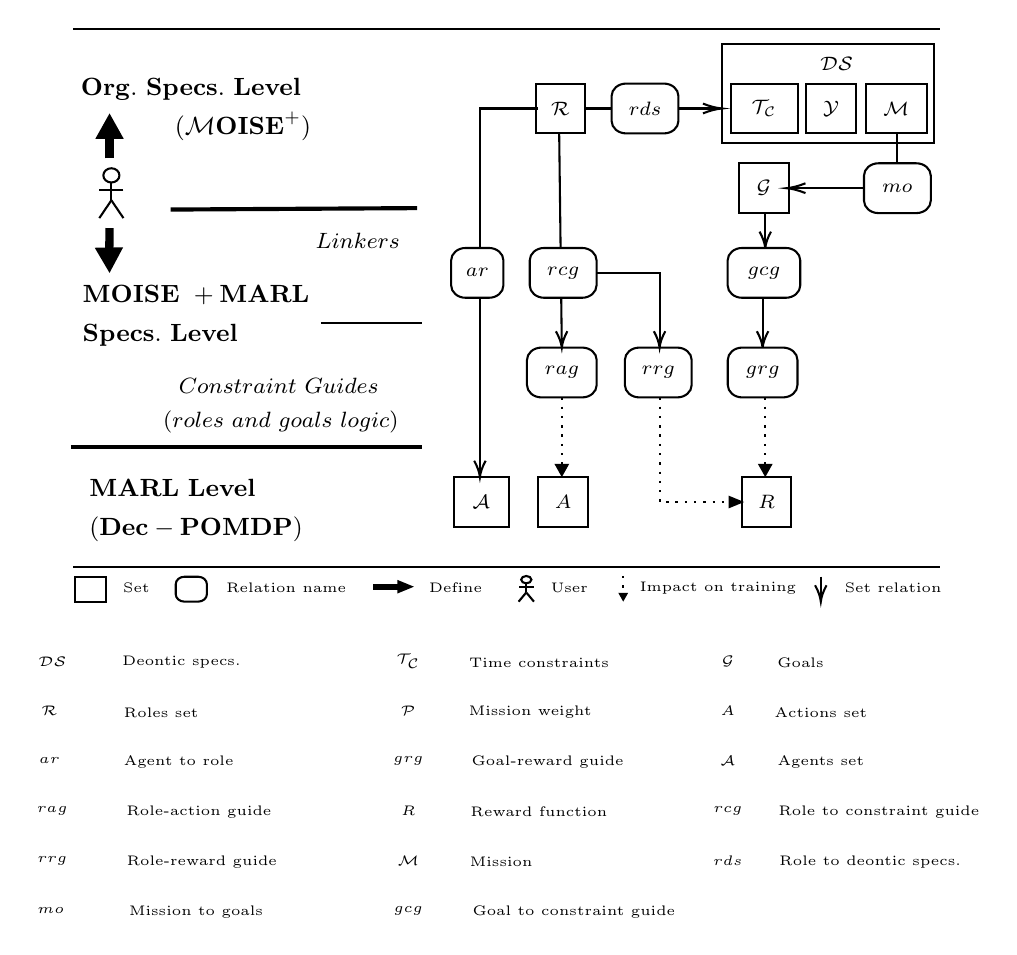
\begin{tikzpicture}[x=0.75pt,y=0.75pt,yscale=-1.2,xscale=1.4]
    %uncomment if require: \path (0,2584); %set diagram left start at 0, and has height of 2584

    %Straight Lines [id:da4973066741986565] 
    \draw [line width=1.5]    (118.21,2302.58) -- (203.1,2302) ;
    %Straight Lines [id:da14807114776731778] 
    \draw    (368.35,2272) -- (368.35,2294) -- (332.16,2294) ;
    \draw [shift={(330.16,2294)}, rotate = 360] [color={rgb, 255:red, 0; green, 0; blue, 0 }  ][line width=0.75]    (6.56,-1.97) .. controls (4.17,-0.84) and (1.99,-0.18) .. (0,0) .. controls (1.99,0.18) and (4.17,0.84) .. (6.56,1.97)   ;
    %Straight Lines [id:da16285043353898754] 
    \draw [line width=1.5]    (83.88,2398) -- (204.61,2398) ;
    %Straight Lines [id:da6299512000169913] 
    \draw    (169.94,2348) -- (204.61,2348) ;
    %Straight Lines [id:da64750232417664] 
    \draw    (84.65,2446) -- (383.15,2446) ;
    %Straight Lines [id:da35895220906699743] 
    \draw    (84.65,2230) -- (383,2230) ;
    %Straight Lines [id:da715014372569708] 
    \draw    (244.68,2262) -- (224.68,2262) -- (224.68,2408) ;
    \draw [shift={(224.68,2410)}, rotate = 270] [color={rgb, 255:red, 0; green, 0; blue, 0 }  ][line width=0.75]    (6.56,-1.97) .. controls (4.17,-0.84) and (1.99,-0.18) .. (0,0) .. controls (1.99,0.18) and (4.17,0.84) .. (6.56,1.97)   ;
    %Straight Lines [id:da71870438525014] 
    \draw    (251.96,2328) -- (286.51,2328) -- (286.51,2356) ;
    \draw [shift={(286.51,2358)}, rotate = 270] [color={rgb, 255:red, 0; green, 0; blue, 0 }  ][line width=0.75]    (6.56,-1.97) .. controls (4.17,-0.84) and (1.99,-0.18) .. (0,0) .. controls (1.99,0.18) and (4.17,0.84) .. (6.56,1.97)   ;
    %Straight Lines [id:da6006267784187092] 
    \draw [line width=0.75]  [dash pattern={on 0.84pt off 2.51pt}]  (252.87,2378) -- (252.87,2407) ;
    \draw [shift={(252.87,2410)}, rotate = 270] [fill={rgb, 255:red, 0; green, 0; blue, 0 }  ][line width=0.08]  [draw opacity=0] (5.36,-2.57) -- (0,0) -- (5.36,2.57) -- cycle    ;
    %Straight Lines [id:da8743336135156266] 
    \draw    (322.88,2304) -- (322.88,2316) ;
    \draw [shift={(322.88,2318)}, rotate = 270] [color={rgb, 255:red, 0; green, 0; blue, 0 }  ][line width=0.75]    (6.56,-1.97) .. controls (4.17,-0.84) and (1.99,-0.18) .. (0,0) .. controls (1.99,0.18) and (4.17,0.84) .. (6.56,1.97)   ;
    %Straight Lines [id:da14641229967966152] 
    \draw [line width=0.75]  [dash pattern={on 0.84pt off 2.51pt}]  (322.88,2378) -- (322.88,2407) ;
    \draw [shift={(322.88,2410)}, rotate = 270] [fill={rgb, 255:red, 0; green, 0; blue, 0 }  ][line width=0.08]  [draw opacity=0] (5.36,-2.57) -- (0,0) -- (5.36,2.57) -- cycle    ;
    %Straight Lines [id:da9260929933425808] 
    \draw [line width=0.75]  [dash pattern={on 0.84pt off 2.51pt}]  (286.51,2378) -- (286.51,2420) -- (312.61,2420) ;
    \draw [shift={(315.61,2420)}, rotate = 180] [fill={rgb, 255:red, 0; green, 0; blue, 0 }  ][line width=0.08]  [draw opacity=0] (5.36,-2.57) -- (0,0) -- (5.36,2.57) -- cycle    ;
    %Straight Lines [id:da3057006030233673] 
    \draw [line width=0.75]  [dash pattern={on 0.84pt off 2.51pt}]  (274,2449.7) -- (274,2457) ;
    \draw [shift={(274,2460)}, rotate = 270] [fill={rgb, 255:red, 0; green, 0; blue, 0 }  ][line width=0.08]  [draw opacity=0] (3.57,-1.72) -- (0,0) -- (3.57,1.72) -- cycle    ;
    %Straight Lines [id:da07288166228322246] 
    \draw    (342,2449.98) -- (342,2458) ;
    \draw [shift={(342,2460)}, rotate = 270] [color={rgb, 255:red, 0; green, 0; blue, 0 }  ][line width=0.75]    (6.56,-1.97) .. controls (4.17,-0.84) and (1.99,-0.18) .. (0,0) .. controls (1.99,0.18) and (4.17,0.84) .. (6.56,1.97)   ;
    %Shape: Ellipse [id:dp8508274348425935] 
    \draw   (95.09,2288.86) .. controls (95.09,2287.28) and (96.33,2286) .. (97.85,2286) .. controls (99.38,2286) and (100.62,2287.28) .. (100.62,2288.86) .. controls (100.62,2290.44) and (99.38,2291.71) .. (97.85,2291.71) .. controls (96.33,2291.71) and (95.09,2290.44) .. (95.09,2288.86) -- cycle ;
    %Straight Lines [id:da3825450168053828] 
    \draw    (97.85,2291.71) -- (97.85,2298.86) ;
    %Straight Lines [id:da521321206042058] 
    \draw    (97.85,2298.86) -- (93.71,2306) ;
    %Straight Lines [id:da055514206493922025] 
    \draw    (97.85,2298.86) -- (102,2306) ;
    %Straight Lines [id:da8996496708356774] 
    \draw    (102,2294.57) -- (93.71,2294.57) ;

    %Straight Lines [id:da31678488015771755] 
    \draw [line width=2.25]    (188,2454) -- (196.97,2454) ;
    \draw [shift={(201.97,2454)}, rotate = 180] [fill={rgb, 255:red, 0; green, 0; blue, 0 }  ][line width=0.08]  [draw opacity=0] (5.72,-2.75) -- (0,0) -- (5.72,2.75) -- cycle    ;
    %Shape: Ellipse [id:dp3927356466672782] 
    \draw   (238.88,2451.17) .. controls (238.88,2450.36) and (239.67,2449.7) .. (240.64,2449.7) .. controls (241.61,2449.7) and (242.4,2450.36) .. (242.4,2451.17) .. controls (242.4,2451.99) and (241.61,2452.65) .. (240.64,2452.65) .. controls (239.67,2452.65) and (238.88,2451.99) .. (238.88,2451.17) -- cycle ;
    %Straight Lines [id:da3365602555559104] 
    \draw    (240.64,2452.65) -- (240.64,2456.32) ;
    %Straight Lines [id:da7990875235744026] 
    \draw    (240.64,2456.32) -- (238,2460) ;
    %Straight Lines [id:da23945649338821617] 
    \draw    (240.64,2456.32) -- (243.28,2460) ;
    %Straight Lines [id:da11927353559661591] 
    \draw    (243.28,2454.12) -- (238,2454.12) ;

    %Straight Lines [id:da5816423191130675] 
    \draw    (251.96,2272) -- (252.85,2356) ;
    \draw [shift={(252.87,2358)}, rotate = 269.39] [color={rgb, 255:red, 0; green, 0; blue, 0 }  ][line width=0.75]    (6.56,-1.97) .. controls (4.17,-0.84) and (1.99,-0.18) .. (0,0) .. controls (1.99,0.18) and (4.17,0.84) .. (6.56,1.97)   ;
    %Straight Lines [id:da9310455126832857] 
    \draw    (321.97,2338) -- (321.97,2356) ;
    \draw [shift={(321.97,2358)}, rotate = 270] [color={rgb, 255:red, 0; green, 0; blue, 0 }  ][line width=0.75]    (6.56,-1.97) .. controls (4.17,-0.84) and (1.99,-0.18) .. (0,0) .. controls (1.99,0.18) and (4.17,0.84) .. (6.56,1.97)   ;
    %Shape: Rectangle [id:dp293492578719597] 
    \draw   (120,2453) .. controls (120,2451.34) and (121.34,2450) .. (123,2450) -- (127.72,2450) .. controls (129.37,2450) and (130.72,2451.34) .. (130.72,2453) -- (130.72,2457) .. controls (130.72,2458.66) and (129.37,2460) .. (127.72,2460) -- (123,2460) .. controls (121.34,2460) and (120,2458.66) .. (120,2457) -- cycle ;
    %Straight Lines [id:da33566712615128225] 
    \draw    (261.05,2262) -- (306,2262) ;
    \draw [shift={(308,2262)}, rotate = 180] [color={rgb, 255:red, 0; green, 0; blue, 0 }  ][line width=0.75]    (6.56,-1.97) .. controls (4.17,-0.84) and (1.99,-0.18) .. (0,0) .. controls (1.99,0.18) and (4.17,0.84) .. (6.56,1.97)   ;
    %Shape: Rectangle [id:dp28383270948937667] 
    \draw   (308,2236) -- (381.08,2236) -- (381.08,2276) -- (308,2276) -- cycle ;
    %Straight Lines [id:da18020989903965012] 
    \draw [line width=3]    (97.22,2282) -- (97.22,2270) ;
    \draw [shift={(97.22,2264)}, rotate = 90] [fill={rgb, 255:red, 0; green, 0; blue, 0 }  ][line width=0.08]  [draw opacity=0] (10.18,-4.89) -- (0,0) -- (10.18,4.89) -- cycle    ;
    %Straight Lines [id:da018421338049046554] 
    \draw [line width=3]    (97.22,2310) -- (97.11,2322.37) ;
    \draw [shift={(97.22,2328)}, rotate = 268.86] [fill={rgb, 255:red, 0; green, 0; blue, 0 }  ][line width=0.08]  [draw opacity=0] (10.18,-4.89) -- (0,0) -- (10.18,4.89) -- cycle    ;
    %Shape: Rectangle [id:dp7281037051878541] 
    \draw   (85.42,2450) -- (96.13,2450) -- (96.13,2460) -- (85.42,2460) -- cycle ;

    % Text Node
    \draw (362,2544.5) node  [font=\tiny] [align=left] {Role to constraint guide};
    % Text Node
    \draw (342,2524.5) node  [font=\tiny] [align=left] {Agents set};
    % Text Node
    \draw (342,2504.5) node  [font=\tiny] [align=left] {Actions set};
    % Text Node
    \draw (257,2584.5) node  [font=\tiny] [align=left] {Goal to constraint guide};
    % Text Node
    \draw (335,2484.5) node  [font=\tiny] [align=left] {Goals};
    % Text Node
    \draw (359,2564.5) node  [font=\tiny] [align=left] {Role to deontic specs.};
    % Text Node
    \draw (232,2564.5) node  [font=\tiny] [align=left] {Mission};
    % Text Node
    \draw (245,2544.5) node  [font=\tiny] [align=left] {Reward function};
    % Text Node
    \draw (248,2524.5) node  [font=\tiny] [align=left] {Goal-reward guide};
    % Text Node
    \draw (242,2504.5) node  [font=\tiny] [align=left] {Mission weight};
    % Text Node
    \draw (245,2484.5) node  [font=\tiny] [align=left] {Time constraints};
    % Text Node
    \draw (127,2584.5) node  [font=\tiny] [align=left] {Mission to goals};
    % Text Node
    \draw (129,2564.5) node  [font=\tiny] [align=left] {Role-reward guide};
    % Text Node
    \draw (128,2544.5) node  [font=\tiny] [align=left] {Role-action guide};
    % Text Node
    \draw (121,2524.5) node  [font=\tiny] [align=left] {Agent to role};
    % Text Node
    \draw (115,2504.5) node  [font=\tiny] [align=left] {Roles set};
    % Text Node
    \draw (122,2484.5) node  [font=\tiny] [align=left] {Deontic specs.};
    % Text Node
    \draw (310,2544) node  [font=\tiny] [align=left] {$\displaystyle \boldsymbol{rcg}$};
    % Text Node
    \draw (200,2504) node  [font=\tiny] [align=left] {$\displaystyle \mathcal{P}$};
    % Text Node
    \draw (200,2484) node  [font=\tiny] [align=left] {$\displaystyle \mathcal{T_{C}}$};
    % Text Node
    \draw (200,2564) node  [font=\tiny] [align=left] {$\displaystyle \mathcal{M}$};
    % Text Node
    \draw (77.5,2484) node  [font=\tiny] [align=left] {$\displaystyle \mathcal{DS}$};
    % Text Node
    \draw (310,2564) node  [font=\tiny] [align=left] {$\displaystyle \boldsymbol{rds}$};
    % Text Node
    \draw (310,2504) node  [font=\tiny] [align=left] {$\displaystyle \boldsymbol{A}$};
    % Text Node
    \draw (200,2544) node  [font=\tiny] [align=left] {$\displaystyle \boldsymbol{R}$};
    % Text Node
    \draw (310,2524) node  [font=\tiny] [align=left] {$\displaystyle \mathcal{A}$};
    % Text Node
    \draw (200,2524) node  [font=\tiny] [align=left] {$\displaystyle \boldsymbol{grg}$};
    % Text Node
    \draw (77.5,2564) node  [font=\tiny] [align=left] {$\displaystyle \boldsymbol{rrg}$};
    % Text Node
    \draw (77.5,2544) node  [font=\tiny] [align=left] {$\displaystyle \boldsymbol{rag}$};
    % Text Node
    \draw (200,2584) node  [font=\tiny] [align=left] {$\displaystyle \boldsymbol{gcg}$};
    % Text Node
    \draw (76.5,2524) node  [font=\tiny] [align=left] {$\displaystyle \boldsymbol{ar}$};
    % Text Node
    \draw (77,2584) node  [font=\tiny] [align=left] {$\displaystyle \boldsymbol{mo}$};
    % Text Node
    \draw (76.5,2504) node  [font=\tiny] [align=left] {$\displaystyle \mathcal{R}$};
    % Text Node
    \draw (310,2484) node  [font=\tiny] [align=left] {$\displaystyle \mathcal{G}$};


    % Text Node
    \draw  [fill={rgb, 255:red, 255; green, 255; blue, 255 }  ,fill opacity=1 ]  (241.82,2323) .. controls (241.82,2320.24) and (244.06,2318) .. (246.82,2318) -- (259.82,2318) .. controls (262.58,2318) and (264.82,2320.24) .. (264.82,2323) -- (264.82,2333) .. controls (264.82,2335.76) and (262.58,2338) .. (259.82,2338) -- (246.82,2338) .. controls (244.06,2338) and (241.82,2335.76) .. (241.82,2333) -- cycle  ;
    \draw (253.32,2328) node  [font=\scriptsize] [align=left] {$\displaystyle \boldsymbol{rcg}$};
    % Text Node
    \draw    (337,2252) -- (354,2252) -- (354,2272) -- (337,2272) -- cycle  ;
    \draw (345.5,2262) node  [font=\scriptsize] [align=left] {$\displaystyle \mathcal{Y}$};
    % Text Node
    \draw    (311,2252) -- (334,2252) -- (334,2272) -- (311,2272) -- cycle  ;
    \draw (322.5,2262) node  [font=\scriptsize] [align=left] {$\displaystyle \mathcal{T_{C}}$};
    % Text Node
    \draw    (357.39,2252) -- (378.39,2252) -- (378.39,2272) -- (357.39,2272) -- cycle  ;
    \draw (367.89,2262) node  [font=\scriptsize] [align=left] {$\displaystyle \mathcal{M}$};
    % Text Node
    \draw (347.43,2244) node  [font=\scriptsize] [align=left] {$\displaystyle \mathcal{DS}$};
    % Text Node
    \draw  [fill={rgb, 255:red, 255; green, 255; blue, 255 }  ,fill opacity=1 ]  (270,2257) .. controls (270,2254.24) and (272.24,2252) .. (275,2252) -- (288,2252) .. controls (290.76,2252) and (293,2254.24) .. (293,2257) -- (293,2267) .. controls (293,2269.76) and (290.76,2272) .. (288,2272) -- (275,2272) .. controls (272.24,2272) and (270,2269.76) .. (270,2267) -- cycle  ;
    \draw (281.5,2262) node  [font=\scriptsize] [align=left] {$\displaystyle \boldsymbol{rds}$};
    % Text Node
    \draw (158,2454.5) node  [font=\tiny] [align=left] {Relation name};
    % Text Node
    \draw (106.46,2454.5) node  [font=\tiny] [align=left] {Set};
    % Text Node
    \draw (255.47,2454.5) node  [font=\tiny] [align=left] {User};
    % Text Node
    \draw (216.32,2454.5) node  [font=\tiny] [align=left] {Define};
    % Text Node
    \draw (366.91,2454.5) node  [font=\tiny] [align=left] {Set relation};
    % Text Node
    \draw (306.61,2454.5) node  [font=\tiny] [align=left] {Impact on training};
    % Text Node
    \draw    (244.82,2410) -- (261.82,2410) -- (261.82,2430) -- (244.82,2430) -- cycle  ;
    \draw (253.32,2420) node  [font=\scriptsize] [align=left] {$\displaystyle \boldsymbol{A}$};
    % Text Node
    \draw    (314.84,2410) -- (331.84,2410) -- (331.84,2430) -- (314.84,2430) -- cycle  ;
    \draw (323.34,2420) node  [font=\scriptsize] [align=left] {$\displaystyle \boldsymbol{R}$};
    % Text Node
    \draw    (215.63,2410) -- (234.63,2410) -- (234.63,2430) -- (215.63,2430) -- cycle  ;
    \draw (225.13,2420) node  [font=\scriptsize] [align=left] {$\displaystyle \mathcal{A}$};
    % Text Node
    \draw  [fill={rgb, 255:red, 255; green, 255; blue, 255 }  ,fill opacity=1 ]  (309.97,2363) .. controls (309.97,2360.24) and (312.21,2358) .. (314.97,2358) -- (328.97,2358) .. controls (331.73,2358) and (333.97,2360.24) .. (333.97,2363) -- (333.97,2373) .. controls (333.97,2375.76) and (331.73,2378) .. (328.97,2378) -- (314.97,2378) .. controls (312.21,2378) and (309.97,2375.76) .. (309.97,2373) -- cycle  ;
    \draw (321.97,2368) node  [font=\scriptsize] [align=left] {$\displaystyle \boldsymbol{grg}$};
    % Text Node
    \draw    (274.56,2363) .. controls (274.56,2360.24) and (276.8,2358) .. (279.56,2358) -- (292.56,2358) .. controls (295.32,2358) and (297.56,2360.24) .. (297.56,2363) -- (297.56,2373) .. controls (297.56,2375.76) and (295.32,2378) .. (292.56,2378) -- (279.56,2378) .. controls (276.8,2378) and (274.56,2375.76) .. (274.56,2373) -- cycle  ;
    \draw (286.06,2368) node  [font=\scriptsize] [align=left] {$\displaystyle \boldsymbol{rrg}$};
    % Text Node
    \draw    (240.87,2363) .. controls (240.87,2360.24) and (243.11,2358) .. (245.87,2358) -- (259.87,2358) .. controls (262.63,2358) and (264.87,2360.24) .. (264.87,2363) -- (264.87,2373) .. controls (264.87,2375.76) and (262.63,2378) .. (259.87,2378) -- (245.87,2378) .. controls (243.11,2378) and (240.87,2375.76) .. (240.87,2373) -- cycle  ;
    \draw (252.87,2368) node  [font=\scriptsize] [align=left] {$\displaystyle \boldsymbol{rag}$};
    % Text Node
    \draw (156.15,2380.5) node  [font=\footnotesize] [align=left] {$\displaystyle  \begin{array}{{>{\displaystyle}l}}
                \ \ \boldsymbol{Constraint\ Guides} \\
                ( roles\ and\ goals\ logic)
            \end{array}$};
    % Text Node
    \draw  [fill={rgb, 255:red, 255; green, 255; blue, 255 }  ,fill opacity=1 ]  (309.93,2323) .. controls (309.93,2320.24) and (312.17,2318) .. (314.93,2318) -- (329.93,2318) .. controls (332.69,2318) and (334.93,2320.24) .. (334.93,2323) -- (334.93,2333) .. controls (334.93,2335.76) and (332.69,2338) .. (329.93,2338) -- (314.93,2338) .. controls (312.17,2338) and (309.93,2335.76) .. (309.93,2333) -- cycle  ;
    \draw (322.43,2328) node  [font=\scriptsize] [align=left] {$\displaystyle \boldsymbol{gcg}$};
    % Text Node
    \draw  [fill={rgb, 255:red, 255; green, 255; blue, 255 }  ,fill opacity=1 ]  (214.77,2323) .. controls (214.77,2320.24) and (217.01,2318) .. (219.77,2318) -- (227.77,2318) .. controls (230.53,2318) and (232.77,2320.24) .. (232.77,2323) -- (232.77,2333) .. controls (232.77,2335.76) and (230.53,2338) .. (227.77,2338) -- (219.77,2338) .. controls (217.01,2338) and (214.77,2335.76) .. (214.77,2333) -- cycle  ;
    \draw (223.77,2328) node  [font=\scriptsize] [align=left] {$\displaystyle \boldsymbol{ar}$};
    % Text Node
    \draw  [fill={rgb, 255:red, 255; green, 255; blue, 255 }  ,fill opacity=1 ]  (356.85,2289) .. controls (356.85,2286.24) and (359.08,2284) .. (361.85,2284) -- (374.85,2284) .. controls (377.61,2284) and (379.85,2286.24) .. (379.85,2289) -- (379.85,2299) .. controls (379.85,2301.76) and (377.61,2304) .. (374.85,2304) -- (361.85,2304) .. controls (359.08,2304) and (356.85,2301.76) .. (356.85,2299) -- cycle  ;
    \draw (368.35,2294) node  [font=\scriptsize] [align=left] {$\displaystyle \boldsymbol{mo}$};
    % Text Node
    \draw (127,2344.5) node  [font=\small] [align=left] {$\displaystyle  \begin{array}{{>{\displaystyle}l}}
                \mathbf{MOISE\ +MARL} \\
                \mathbf{Specs.\ Level}
            \end{array}$};
    % Text Node
    \draw (127,2422.5) node  [font=\small] [align=left] {$\displaystyle  \begin{array}{{>{\displaystyle}l}}
                \mathbf{MARL\ Level} \\
                \mathbf{(Dec-POMDP)}
            \end{array}$};
    % Text Node
    \draw    (243.91,2252) -- (260.91,2252) -- (260.91,2272) -- (243.91,2272) -- cycle  ;
    \draw (252.41,2262) node  [font=\scriptsize] [align=left] {$\displaystyle \mathcal{R}$};
    % Text Node
    \draw (182.64,2315) node  [font=\footnotesize] [align=left] {$\displaystyle \boldsymbol{Linkers}$};
    % Text Node
    \draw    (313.93,2284) -- (330.93,2284) -- (330.93,2304) -- (313.93,2304) -- cycle  ;
    \draw (322.43,2294) node  [font=\scriptsize] [align=left] {$\displaystyle \mathcal{G}$};
    % Text Node
    \draw (127,2261.5) node  [font=\small] [align=left] {$\displaystyle  \begin{array}{{>{\displaystyle}l}}
                \mathbf{{\displaystyle Org.\ Specs.\ Level}} \\
                {\displaystyle \ \ \ \ \ \ \ \ \ \ \ (\mathcal{M}\mathbf{OISE^+})}
            \end{array}$};


\end{tikzpicture}
    \caption{Une vue minimale du cadre MOISE+MARL :
        Les utilisateurs commencent par définir les spécifications $\mathcal{M}OISE^+$, qui incluent les rôles ($\mathcal{R}$) et les missions ($\mathcal{M}$), tous deux associés via la relation $rds$.  
        Ils créent ensuite les spécifications MOISE+MARL en définissant d'abord les \textbf{guides de contrainte}, tels que $rag$ et $rrg$ pour spécifier la logique des rôles, et $grg$ pour la logique des objectifs.  
        Puis, les \textbf{lieurs} (\textit{linkers}) sont utilisés pour relier les agents aux rôles via $ar$, et pour connecter la logique des guides de contrainte aux spécifications $\mathcal{M}OISE^+$ définies.  
        Une fois cette configuration en place, les rôles peuvent être attribués aux agents, et le cadre MARL s'adapte automatiquement durant l'apprentissage.}
    \label{fig:mm_synthesis}
\end{figure}

\

\noindent Les \textbf{Guides de Contrainte} sont trois relations introduites pour modéliser la logique des rôles et objectifs de $\mathcal{M}OISE^+$ dans le formalisme Dec-POMDP :

\begin{enumerate}[label={\roman*) },itemjoin={; \quad}]
    \item \textbf{Guide d'Action de Rôle} \quad $rag: H \times \Omega \rightarrow \mathcal{P}(A \times \mathbb{R})$ : cette relation modélise un rôle comme un ensemble de règles associant, à chaque paire composée d'un historique $h \in H$ et d'une observation $\omega \in \Omega$, un ensemble d'actions attendues $A \in \mathcal{P}(A)$ chacune associée à un niveau de contrainte $ch \in [0,1]$ (avec $ch = 1$ par défaut). En restreignant le choix de l'action suivante, l'agent est incité à se conformer au comportement attendu pour son rôle ;
    
    \item \textbf{Guide de Récompense de Rôle} \quad $rrg: H \times \Omega \times A \to \mathbb{R} = \{r_m \text{ si } a \notin A_\omega, \text{ avec } rag(h, \omega) = A_\omega \times \mathbb{R}, h \in H; \text{ sinon } 0\}$ : cette relation ajoute une pénalité $r_m$ à la récompense globale si l'action $a \in A$ choisie n'est pas autorisée. Elle encourage ainsi le respect du comportement attendu ;
    
    \item \textbf{Guide de Récompense d'Objectif} \quad $grg: H \rightarrow \mathbb{R}$ : cette relation modélise un objectif comme une contrainte souple qui ajoute un bonus $r_b \in \mathbb{R}$ à la récompense si l'historique $h \in H$ de l'agent contient une sous-séquence caractéristique $h_g \in H_g$ d'un objectif, l'encourageant ainsi à le réaliser.
\end{enumerate}

\vspace{0.8em}

\noindent Nous introduisons également les \textbf{Lieurs} (\textit{Linkers}) pour connecter les spécifications organisationnelles de $\mathcal{M}OISE^+$ aux guides de contrainte et aux agents :

\begin{enumerate}[label={\roman*) },itemjoin={; \quad}]
    \item \textbf{Agent vers Rôle} \quad $ar: \mathcal{A} \to \mathcal{R}$ : relation bijective associant un agent à un rôle ;
    
    \item \textbf{Rôle vers Guide de Contrainte} \quad $rcg: \mathcal{R} \rightarrow rag \cup rrg$ : relie chaque rôle $\mathcal{M}OISE^+$ à un guide $rag$ ou $rrg$ pour contraindre ou encourager l'agent à suivre les actions attendues ;
    
    \item \textbf{Objectif vers Guide de Contrainte} \quad $gcg: \mathcal{G} \rightarrow grg$ : relie les objectifs à des guides $grg$, les représentant sous forme de récompenses dans le MARL.
\end{enumerate}

\paragraph{\textbf{Résolution du Dec-POMDP avec MOISE+MARL}}

\begin{figure*}[h]
    \label{eq:single_value_function}
    \raggedright
    \textbf{\textit{Definition 1} \quad State-Value function adapted to constraint guides in AEC:}
    
    \begin{scriptsize}
        \vspace{-0.6cm}
        \begin{gather*}
            V^{\pi^j}(s_t) = \hspace{-0.75cm}
            %
            \sum_{\textcolor{red}{ \substack{a_{t} \in A \text{ si } rn() < ch_{t}, \\
                        a_{t} \in A_{t} \text{ else}}
                }}{\hspace{-0.7cm} \pi_i(a_{t} | \omega_t)}
            %
            \sum_{s_{t+1} \in S}
            %    
            {\hspace{-0.1cm} T(s_{t+1} | s_t, a_{t})
            \Bigl[R(s_t,a_{t},s_{t+1}) + \hspace{-0.1cm}
            \textcolor{blue}{ \sum_{m \in \mathcal{M}_i}{ \hspace{-0.1cm} v_m(t) \frac{grg_m(h_{t+1})}{1 - p + \epsilon} } }
            + } \\
            {\textcolor{red}{(1-ch_t) \times rrg(\omega_t,a_{t+1})} + V^{\pi^j_{i+1 \ mod \ n}}(s_{t+1})\Bigr]}
        \end{gather*}
        %
        \vspace{-0.5cm}
        \textcolor{red}{\[\text{ \hspace{-0.1cm} With } rag(h_t, \omega_t) = A_{t} \times \mathbb{R} \text{, } \langle a_t, ch_{t} \rangle \in A_{t} \times \mathbb{R} \text{ ; } rn: \emptyset \to [0,1[ \text{, a uniform random function}\]}
        %
        \vspace{-0.6cm}
        \textcolor{blue}{
            \begin{gather*}
                \hspace{-0.001cm}
                \text{With } \omega_t = O(\omega_t | s_t, a_t) \text{ ; } h_t = \{h_0 = \langle \rangle, h_{t+1} = \langle h_t, \langle \omega_{t+1}, a_{t+1} \rangle \rangle \} \text{ ; } \epsilon \in \mathbb{R}_{>0} \text{ ; } grg_m(h) = 
            \end{gather*}
        }
        \vspace{-0.95cm}
        \textcolor{blue}{
            \begin{gather*}
                \hspace{-0.5cm} \sum_{\hspace{0.3cm}(grg_i,w_i) \in mo(m)}{\hspace{-0.9cm} w_i \times grg_i(h)}
                \text{ ; } v_m(t) = \{ 1 \text{ if } t \in t_c \text{ ; else } 0 \} \text{ ; } \mathcal{M}_i = \{m_j | \langle ar(i),m_j,t_c,p \rangle \in \mathcal{M}\}
            \end{gather*}
        }
        \vspace{-0.6cm}
    \end{scriptsize}
    
\end{figure*}

Un modèle MOISE+MARL est formalisé par $MM = \langle \mathcal{OS}, ar, rcg, gcg, rag, rrg, grg\rangle$.

La résolution d'un Dec-POMDP $d \in D$ avec un modèle $mm \in \mathcal{MM}$ consiste à trouver une politique conjointe $\pi^{j} = \{\pi^j_0, \pi^j_1, \dots, \pi^j_n\}$ qui maximise la fonction de valeur d'état $V^{\pi^{j}}$ (ou atteint un seuil minimal), représentant la récompense cumulative attendue à partir d'un état initial $s \in S$, en suivant la politique $\pi^{j}$ et en appliquant des actions conjointes $a^{j} \in A^n$ sous l'effet des guides de contrainte supplémentaires.

Cette fonction est décrite dans le cas où les agents agissent séquentiellement et cycliquement (mode Agent Environment Cycle - AEC) dans la \hyperref[eq:single_value_function]{Définition 1}. Celle-ci adapte sa définition pour refléter l'impact des rôles (en rouge) et des missions (en bleu), influant à la fois sur l'espace d'actions et la récompense. La \autoref{fig:mm_synthesis} illustre les liens entre $\mathcal{M}OISE^+$ et Dec-POMDP à travers le cadre MOISE+MARL.

À chaque instant $t \in \mathbb{N}$ (initialement $t = 0$), l'agent $i = t \mod n$ est associé à un rôle $\rho_i = ar(i)$. Pour chaque spécification déontique valide $d_i = rds(\rho_i) = \langle tc_i, y_i, m_i \rangle$, l'agent est soit autorisé (si $y_i = 0$), soit obligé (si $y_i = 1$) à s'engager dans la mission $m_i \in \mathcal{M}$, avec $\mathcal{G}_{m_i} = mo(m_i)$ et $n \in \mathbb{N}$ le nombre d'agents.

Ensuite, à partir de l'observation reçue $\omega_t$, l'agent choisit une action selon :
i) l'ensemble des actions attendues $A_t$ si une valeur aléatoire est inférieure à la dureté de contrainte $ch_t$ ;
ii) ou l'ensemble complet $A$ sinon.

Lorsque $ch_t = 1$, le rôle est fortement contraignant ; sinon, il est faiblement prescriptif.

L'action choisie est appliquée à l'état $s_t$ pour générer une transition vers l'état $s_{t+1}$, produire l'observation $\omega_{t+1}$, et calculer une récompense.

Cette récompense est composée de :
i) la somme des bonus liés aux objectifs atteints, pour chaque mission valide temporellement (via les guides $grg$), pondérée par $\frac{1}{1 - p + \epsilon}$ ;
ii) la pénalité induite par les écarts au comportement de rôle attendu (via les guides $rrg$), pondérée par $1 - ch_t$.

Le calcul de la récompense cumulative se poursuit ensuite dans l'état suivant $s_{t+1} \in S$ avec l'agent suivant $(i+1) \mod n$.

\subsubsection{Apprentissage de World Models}

En apprentissage par renforcement (RL), notamment en contexte d'observabilité partielle, les \textbf{World Models} (\textit{World Models})~\cite{ha2018recurrent} visent à approximer les fonctions de transition et d'observation d'un Processus Décisionnel de Markov Partiellement Observable (POMDP). Ils permettent ainsi la planification, l'exploration sûre et un apprentissage de politiques plus efficace. Cette approche appartient au paradigme de l'\textit{apprentissage par renforcement basé sur un modèle} (\textit{Model-Based RL} – MBRL)~\cite{moerland2020model}. Elle est particulièrement utile pour capturer automatiquement la complexité d'un environnement sous la forme d'un modèle type simulation, sans représentation explicite de l'environnement.

Soit $\omega_t \in \Omega$ l'observation et $a_t \in \mathcal{A}$ l'action à l'instant $t$. Le cœur d'un World Model consiste à approximer la \textbf{fonction de dynamique observable} $\mathcal{T}: \Omega \times A \rightarrow \Omega$, qui capture la transition d'état caché et les dynamiques observables. En pratique, cette fonction est souvent implémentée à l'aide de réseaux neuronaux récurrents (RNN), notamment les réseaux à mémoire long-court terme (LSTM)~\cite{hochreiter1997long}, pour modéliser la dimension temporelle. Toutefois, comme les observations sont souvent de grande dimension, un encodeur $Enc: \Omega \rightarrow Z$ est utilisé pour extraire une représentation latente réduite, et un décodeur $Dec: Z \rightarrow \Omega$ permet de reconstruire l'observation à partir de cette représentation.

\[
    z_t = Enc(\omega_t), \quad
    z_{t+1} = \mathcal{T}(z_t, a_t), \quad
    \hat{\omega}_{t+1} = Dec(z_{t+1}),
\]

où $\forall z \in Z, \omega \in \Omega, \dim(z) \leq \dim(\omega)$, en considérant l'observation $\omega$ comme un vecteur. L'entraînement du modèle vise à minimiser la perte de reconstruction $\|\omega_{t+1} - \hat{\omega}_{t+1}\|$, ainsi qu'une perte de prédiction dans l'espace latent.

Dans un contexte multi-agent, la modélisation du monde doit prendre en compte la dynamique décentralisée~\cite{yang2021representation}. La fonction de dynamique observable traite alors les observations et actions conjointes, ainsi que leurs représentations latentes respectives. Dans le cadre de MAMAD, les World Models constituent le noyau de simulation de la phase de \hyperref[sec:modelling]{modélisation}, agissant comme des jumeaux numériques.



\subsection{La méthode MAMAD}\label{sec:mamad}

\subsubsection{Vue d'ensemble de la méthode}

La méthode MAMAD~\footnote{Le code source et les détails de MAMAD sont disponibles à l'adresse \url{https://github.com/julien6/MAMAD}} s'articule autour de quatre grandes phases :  
(1) modélisation de l'environnement, des objectifs globaux et des contraintes organisationnelles selon le cadre proposé ;  
(2) apprentissage des politiques à l'aide de différents algorithmes MARL ;  
(3) analyse des comportements et inférence des spécifications organisationnelles à l'aide d'une méthode dédiée ;  
(4) développement et déploiement du SMA.  

Cette approche guide le processus d'apprentissage des agents tout en appliquant des contraintes organisationnelles strictes, garantissant l'efficacité des politiques apprises. Le cycle de vie d'un SMA conçu avec MAMAD est illustré en \autoref{fig:cycle}.

\begin{figure}[h!]
    \centering
    


\tikzset{every picture/.style={line width=0.75pt}} %set default line width to 0.75pt        

\begin{tikzpicture}[x=0.75pt,y=0.75pt,yscale=-1,xscale=1]
%uncomment if require: \path (0,3307); %set diagram left start at 0, and has height of 3307

%Shape: Smiley Face [id:dp29065495216725257] 
\draw  [line width=1.5]  (85.38,2800.11) .. controls (85.38,2797.7) and (87.16,2795.75) .. (89.36,2795.75) .. controls (91.55,2795.75) and (93.34,2797.7) .. (93.34,2800.11) .. controls (93.34,2802.52) and (91.55,2804.48) .. (89.36,2804.48) .. controls (87.16,2804.48) and (85.38,2802.52) .. (85.38,2800.11) -- cycle ; \draw  [line width=1.5]  (87.61,2798.63) .. controls (87.61,2798.39) and (87.78,2798.19) .. (88,2798.19) .. controls (88.22,2798.19) and (88.4,2798.39) .. (88.4,2798.63) .. controls (88.4,2798.87) and (88.22,2799.07) .. (88,2799.07) .. controls (87.78,2799.07) and (87.61,2798.87) .. (87.61,2798.63) -- cycle ; \draw  [line width=1.5]  (90.31,2798.63) .. controls (90.31,2798.39) and (90.49,2798.19) .. (90.71,2798.19) .. controls (90.93,2798.19) and (91.11,2798.39) .. (91.11,2798.63) .. controls (91.11,2798.87) and (90.93,2799.07) .. (90.71,2799.07) .. controls (90.49,2799.07) and (90.31,2798.87) .. (90.31,2798.63) -- cycle ; \draw  [line width=1.5]  (87.37,2801.86) .. controls (88.69,2803.02) and (90.02,2803.02) .. (91.35,2801.86) ;
%Shape: Rectangle [id:dp42672371521059915] 
\draw  [dash pattern={on 5.63pt off 4.5pt}][line width=1.5]  (74.03,2763.75) -- (192,2763.75) -- (192,2813.93) -- (74.03,2813.93) -- cycle ;
%Shape: Smiley Face [id:dp9817389082285293] 
\draw  [line width=1.5]  (144.45,2803.6) .. controls (144.45,2801.19) and (146.24,2799.24) .. (148.43,2799.24) .. controls (150.63,2799.24) and (152.41,2801.19) .. (152.41,2803.6) .. controls (152.41,2806.01) and (150.63,2807.97) .. (148.43,2807.97) .. controls (146.24,2807.97) and (144.45,2806.01) .. (144.45,2803.6) -- cycle ; \draw  [line width=1.5]  (146.68,2802.12) .. controls (146.68,2801.88) and (146.86,2801.68) .. (147.08,2801.68) .. controls (147.3,2801.68) and (147.48,2801.88) .. (147.48,2802.12) .. controls (147.48,2802.36) and (147.3,2802.56) .. (147.08,2802.56) .. controls (146.86,2802.56) and (146.68,2802.36) .. (146.68,2802.12) -- cycle ; \draw  [line width=1.5]  (149.39,2802.12) .. controls (149.39,2801.88) and (149.57,2801.68) .. (149.79,2801.68) .. controls (150.01,2801.68) and (150.18,2801.88) .. (150.18,2802.12) .. controls (150.18,2802.36) and (150.01,2802.56) .. (149.79,2802.56) .. controls (149.57,2802.56) and (149.39,2802.36) .. (149.39,2802.12) -- cycle ; \draw  [line width=1.5]  (146.44,2805.35) .. controls (147.77,2806.51) and (149.1,2806.51) .. (150.42,2805.35) ;
%Shape: Smiley Face [id:dp49419175504212776] 
\draw  [line width=1.5]  (179.09,2781.5) .. controls (179.09,2779.09) and (180.87,2777.13) .. (183.06,2777.13) .. controls (185.26,2777.13) and (187.04,2779.09) .. (187.04,2781.5) .. controls (187.04,2783.91) and (185.26,2785.86) .. (183.06,2785.86) .. controls (180.87,2785.86) and (179.09,2783.91) .. (179.09,2781.5) -- cycle ; \draw  [line width=1.5]  (181.31,2780.01) .. controls (181.31,2779.77) and (181.49,2779.58) .. (181.71,2779.58) .. controls (181.93,2779.58) and (182.11,2779.77) .. (182.11,2780.01) .. controls (182.11,2780.25) and (181.93,2780.45) .. (181.71,2780.45) .. controls (181.49,2780.45) and (181.31,2780.25) .. (181.31,2780.01) -- cycle ; \draw  [line width=1.5]  (184.02,2780.01) .. controls (184.02,2779.77) and (184.2,2779.58) .. (184.42,2779.58) .. controls (184.64,2779.58) and (184.81,2779.77) .. (184.81,2780.01) .. controls (184.81,2780.25) and (184.64,2780.45) .. (184.42,2780.45) .. controls (184.2,2780.45) and (184.02,2780.25) .. (184.02,2780.01) -- cycle ; \draw  [line width=1.5]  (181.07,2783.24) .. controls (182.4,2784.4) and (183.73,2784.4) .. (185.05,2783.24) ;
%Flowchart: Punched Tape [id:dp3565745198144521] 
\draw  [fill={rgb, 255:red, 255; green, 255; blue, 255 }  ,fill opacity=1 ] (291.67,2877.34) .. controls (291.67,2880.23) and (301.36,2882.58) .. (313.31,2882.58) .. controls (325.26,2882.58) and (334.95,2880.23) .. (334.95,2877.34) .. controls (334.95,2874.45) and (344.64,2872.11) .. (356.6,2872.11) .. controls (368.55,2872.11) and (378.24,2874.45) .. (378.24,2877.34) -- (378.24,2919.23) .. controls (378.24,2916.34) and (368.55,2913.99) .. (356.6,2913.99) .. controls (344.64,2913.99) and (334.95,2916.34) .. (334.95,2919.23) .. controls (334.95,2922.12) and (325.26,2924.46) .. (313.31,2924.46) .. controls (301.36,2924.46) and (291.67,2922.12) .. (291.67,2919.23) -- cycle ;
%Straight Lines [id:da23451091058783402] 
\draw [line width=1.5]    (320.63,2891.89) -- (349.47,2889.91) ;
\draw [shift={(352.46,2889.7)}, rotate = 176.08] [color={rgb, 255:red, 0; green, 0; blue, 0 }  ][line width=1.5]    (8.53,-2.57) .. controls (5.42,-1.09) and (2.58,-0.23) .. (0,0) .. controls (2.58,0.23) and (5.42,1.09) .. (8.53,2.57)   ;
%Straight Lines [id:da05993633349010663] 
\draw [line width=1.5]    (320.63,2894.07) -- (335.84,2901.48) ;
\draw [shift={(338.53,2902.79)}, rotate = 205.98] [color={rgb, 255:red, 0; green, 0; blue, 0 }  ][line width=1.5]    (8.53,-2.57) .. controls (5.42,-1.09) and (2.58,-0.23) .. (0,0) .. controls (2.58,0.23) and (5.42,1.09) .. (8.53,2.57)   ;
%Shape: Smiley Face [id:dp5316832937595011] 
\draw  [line width=1.5]  (312.91,2893.34) .. controls (312.91,2890.93) and (314.69,2888.98) .. (316.89,2888.98) .. controls (319.09,2888.98) and (320.87,2890.93) .. (320.87,2893.34) .. controls (320.87,2895.75) and (319.09,2897.7) .. (316.89,2897.7) .. controls (314.69,2897.7) and (312.91,2895.75) .. (312.91,2893.34) -- cycle ; \draw  [line width=1.5]  (315.14,2891.86) .. controls (315.14,2891.61) and (315.32,2891.42) .. (315.54,2891.42) .. controls (315.76,2891.42) and (315.94,2891.61) .. (315.94,2891.86) .. controls (315.94,2892.1) and (315.76,2892.29) .. (315.54,2892.29) .. controls (315.32,2892.29) and (315.14,2892.1) .. (315.14,2891.86) -- cycle ; \draw  [line width=1.5]  (317.85,2891.86) .. controls (317.85,2891.61) and (318.02,2891.42) .. (318.24,2891.42) .. controls (318.46,2891.42) and (318.64,2891.61) .. (318.64,2891.86) .. controls (318.64,2892.1) and (318.46,2892.29) .. (318.24,2892.29) .. controls (318.02,2892.29) and (317.85,2892.1) .. (317.85,2891.86) -- cycle ; \draw  [line width=1.5]  (314.9,2895.08) .. controls (316.23,2896.25) and (317.55,2896.25) .. (318.88,2895.08) ;
%Shape: Smiley Face [id:dp5491508300746957] 
\draw  [line width=1.5]  (338.38,2904.97) .. controls (338.38,2902.56) and (340.16,2900.61) .. (342.35,2900.61) .. controls (344.55,2900.61) and (346.33,2902.56) .. (346.33,2904.97) .. controls (346.33,2907.38) and (344.55,2909.34) .. (342.35,2909.34) .. controls (340.16,2909.34) and (338.38,2907.38) .. (338.38,2904.97) -- cycle ; \draw  [line width=1.5]  (340.6,2903.49) .. controls (340.6,2903.25) and (340.78,2903.05) .. (341,2903.05) .. controls (341.22,2903.05) and (341.4,2903.25) .. (341.4,2903.49) .. controls (341.4,2903.73) and (341.22,2903.93) .. (341,2903.93) .. controls (340.78,2903.93) and (340.6,2903.73) .. (340.6,2903.49) -- cycle ; \draw  [line width=1.5]  (343.31,2903.49) .. controls (343.31,2903.25) and (343.49,2903.05) .. (343.71,2903.05) .. controls (343.93,2903.05) and (344.1,2903.25) .. (344.1,2903.49) .. controls (344.1,2903.73) and (343.93,2903.93) .. (343.71,2903.93) .. controls (343.49,2903.93) and (343.31,2903.73) .. (343.31,2903.49) -- cycle ; \draw  [line width=1.5]  (340.36,2906.72) .. controls (341.69,2907.88) and (343.02,2907.88) .. (344.34,2906.72) ;
%Shape: Smiley Face [id:dp21362593128550156] 
\draw  [line width=1.5]  (352.64,2888.69) .. controls (352.64,2886.28) and (354.42,2884.32) .. (356.61,2884.32) .. controls (358.81,2884.32) and (360.59,2886.28) .. (360.59,2888.69) .. controls (360.59,2891.1) and (358.81,2893.05) .. (356.61,2893.05) .. controls (354.42,2893.05) and (352.64,2891.1) .. (352.64,2888.69) -- cycle ; \draw  [line width=1.5]  (354.86,2887.2) .. controls (354.86,2886.96) and (355.04,2886.77) .. (355.26,2886.77) .. controls (355.48,2886.77) and (355.66,2886.96) .. (355.66,2887.2) .. controls (355.66,2887.44) and (355.48,2887.64) .. (355.26,2887.64) .. controls (355.04,2887.64) and (354.86,2887.44) .. (354.86,2887.2) -- cycle ; \draw  [line width=1.5]  (357.57,2887.2) .. controls (357.57,2886.96) and (357.75,2886.77) .. (357.97,2886.77) .. controls (358.19,2886.77) and (358.36,2886.96) .. (358.36,2887.2) .. controls (358.36,2887.44) and (358.19,2887.64) .. (357.97,2887.64) .. controls (357.75,2887.64) and (357.57,2887.44) .. (357.57,2887.2) -- cycle ; \draw  [line width=1.5]  (354.62,2890.43) .. controls (355.95,2891.59) and (357.28,2891.59) .. (358.6,2890.43) ;
%Left Arrow [id:dp22187584774212898] 
\draw   (215,2804.55) -- (220.28,2802) -- (220.28,2803.27) -- (263.54,2803.27) -- (263.54,2805.82) -- (220.28,2805.82) -- (220.28,2807.09) -- cycle ;
%Left Arrow [id:dp1861077704673879] 
\draw   (315.35,2834) -- (317.89,2837.8) -- (316.62,2837.8) -- (316.62,2868.91) -- (314.07,2868.91) -- (314.07,2837.8) -- (312.8,2837.8) -- cycle ;
%Left Arrow [id:dp2590948740182193] 
\draw   (130.55,2868.91) -- (128,2865.11) -- (129.27,2865.11) -- (129.27,2834) -- (131.82,2834) -- (131.82,2865.11) -- (133.09,2865.11) -- cycle ;
%Left Arrow [id:dp7631269314674067] 
\draw   (262.54,2900.55) -- (257.26,2903.09) -- (257.26,2901.82) -- (214,2901.82) -- (214,2899.27) -- (257.26,2899.27) -- (257.26,2898) -- cycle ;
%Shape: Arc [id:dp8010751146858193] 
\draw  [draw opacity=0] (78.55,2898.86) .. controls (77.97,2897.43) and (79.7,2895.07) .. (82.41,2893.59) .. controls (85.13,2892.11) and (87.81,2892.08) .. (88.39,2893.51) -- (83.47,2896.19) -- cycle ; \draw   (78.55,2898.86) .. controls (77.97,2897.43) and (79.7,2895.07) .. (82.41,2893.59) .. controls (85.13,2892.11) and (87.81,2892.08) .. (88.39,2893.51) ;  
%Shape: Arc [id:dp2168479262754166] 
\draw  [draw opacity=0] (79.96,2900.21) .. controls (79.37,2898.78) and (80.79,2896.59) .. (83.12,2895.32) .. controls (85.45,2894.06) and (87.81,2894.19) .. (88.39,2895.63) -- (84.17,2897.92) -- cycle ; \draw   (79.96,2900.21) .. controls (79.37,2898.78) and (80.79,2896.59) .. (83.12,2895.32) .. controls (85.45,2894.06) and (87.81,2894.19) .. (88.39,2895.63) ;  
%Shape: Arc [id:dp1657064934185728] 
\draw  [draw opacity=0] (81.36,2901.56) .. controls (81.36,2901.56) and (81.36,2901.56) .. (81.36,2901.56) .. controls (80.78,2900.13) and (81.88,2898.11) .. (83.82,2897.06) .. controls (85.76,2896) and (87.81,2896.31) .. (88.39,2897.74) -- (84.88,2899.65) -- cycle ; \draw   (81.36,2901.56) .. controls (81.36,2901.56) and (81.36,2901.56) .. (81.36,2901.56) .. controls (80.78,2900.13) and (81.88,2898.11) .. (83.82,2897.06) .. controls (85.76,2896) and (87.81,2896.31) .. (88.39,2897.74) ;  
%Shape: Arc [id:dp6696163073703636] 
\draw  [draw opacity=0] (82.77,2902.92) .. controls (82.77,2902.92) and (82.77,2902.92) .. (82.77,2902.92) .. controls (82.77,2902.92) and (82.77,2902.92) .. (82.77,2902.92) .. controls (82.19,2901.48) and (82.97,2899.63) .. (84.53,2898.79) .. controls (86.08,2897.94) and (87.81,2898.42) .. (88.39,2899.86) -- (85.58,2901.39) -- cycle ; \draw   (82.77,2902.92) .. controls (82.77,2902.92) and (82.77,2902.92) .. (82.77,2902.92) .. controls (82.77,2902.92) and (82.77,2902.92) .. (82.77,2902.92) .. controls (82.19,2901.48) and (82.97,2899.63) .. (84.53,2898.79) .. controls (86.08,2897.94) and (87.81,2898.42) .. (88.39,2899.86) ;  
%Shape: Arc [id:dp5914598807756752] 
\draw  [draw opacity=0] (84.18,2904.27) .. controls (83.6,2902.83) and (84.07,2901.15) .. (85.23,2900.52) .. controls (86.4,2899.89) and (87.81,2900.54) .. (88.4,2901.97) -- (86.29,2903.12) -- cycle ; \draw   (84.18,2904.27) .. controls (83.6,2902.83) and (84.07,2901.15) .. (85.23,2900.52) .. controls (86.4,2899.89) and (87.81,2900.54) .. (88.4,2901.97) ;  

%Image [id:dp3722282424817167] 
\draw (291.67,2795.75) node  {
\includegraphics[width=7.64pt,height=13.09pt]{figures/robot.png}};
%Shape: Rectangle [id:dp9197785817800539] 
\draw  [line width=1.5]  (275.37,2763.75) -- (390.8,2763.75) -- (390.8,2813.93) -- (275.37,2813.93) -- cycle ;
%Image [id:dp9715658782589778] 
\draw (382.32,2779.46) node  {
\includegraphics[width=7.64pt,height=13.09pt]{figures/robot.png}};
%Image [id:dp635616861971029] 
\draw (352.78,2801.57) node  {
\includegraphics[width=7.64pt,height=13.09pt]{figures/robot.png}};
%Shape: Rectangle [id:dp647928357040308] 
\draw  [fill={rgb, 255:red, 0; green, 0; blue, 0 }  ,fill opacity=1 ] (291.67,2769.57) -- (301.85,2769.57) -- (301.85,2781.21) -- (291.67,2781.21) -- cycle ;
%Shape: Rectangle [id:dp9626828362725837] 
\draw  [fill={rgb, 255:red, 0; green, 0; blue, 0 }  ,fill opacity=1 ] (373.15,2792.84) -- (383.33,2792.84) -- (383.33,2804.48) -- (373.15,2804.48) -- cycle ;
%Shape: Ellipse [id:dp6171740062199291] 
\draw  [fill={rgb, 255:red, 0; green, 0; blue, 0 }  ,fill opacity=1 ] (347.69,2775.39) .. controls (347.69,2772.17) and (349.97,2769.57) .. (352.78,2769.57) .. controls (355.59,2769.57) and (357.87,2772.17) .. (357.87,2775.39) .. controls (357.87,2778.6) and (355.59,2781.21) .. (352.78,2781.21) .. controls (349.97,2781.21) and (347.69,2778.6) .. (347.69,2775.39) -- cycle ;
%Shape: Triangle [id:dp8145134127966778] 
\draw  [fill={rgb, 255:red, 0; green, 0; blue, 0 }  ,fill opacity=1 ] (322.22,2792.84) -- (327.31,2804.48) -- (317.13,2804.48) -- cycle ;
%Shape: Rectangle [id:dp07981685971419106] 
\draw  [fill={rgb, 255:red, 0; green, 0; blue, 0 }  ,fill opacity=1 ] (89.45,2769.57) -- (99.64,2769.57) -- (99.64,2781.21) -- (89.45,2781.21) -- cycle ;
%Shape: Rectangle [id:dp9786998324005067] 
\draw  [fill={rgb, 255:red, 0; green, 0; blue, 0 }  ,fill opacity=1 ] (170.94,2792.84) -- (181.12,2792.84) -- (181.12,2804.48) -- (170.94,2804.48) -- cycle ;
%Shape: Ellipse [id:dp6465785854464419] 
\draw  [fill={rgb, 255:red, 0; green, 0; blue, 0 }  ,fill opacity=1 ] (145.47,2775.39) .. controls (145.47,2772.17) and (147.75,2769.57) .. (150.57,2769.57) .. controls (153.38,2769.57) and (155.66,2772.17) .. (155.66,2775.39) .. controls (155.66,2778.6) and (153.38,2781.21) .. (150.57,2781.21) .. controls (147.75,2781.21) and (145.47,2778.6) .. (145.47,2775.39) -- cycle ;
%Shape: Triangle [id:dp5909890868954251] 
\draw  [fill={rgb, 255:red, 0; green, 0; blue, 0 }  ,fill opacity=1 ] (120.01,2792.84) -- (125.1,2804.48) -- (114.92,2804.48) -- cycle ;
%Shape: Smiley Face [id:dp661163164093121] 
\draw  [line width=1.5]  (85.52,2909.38) .. controls (85.52,2906.98) and (87.3,2905.03) .. (89.5,2905.03) .. controls (91.7,2905.03) and (93.48,2906.98) .. (93.48,2909.38) .. controls (93.48,2911.78) and (91.7,2913.73) .. (89.5,2913.73) .. controls (87.3,2913.73) and (85.52,2911.78) .. (85.52,2909.38) -- cycle ; \draw  [line width=1.5]  (87.75,2907.9) .. controls (87.75,2907.66) and (87.93,2907.46) .. (88.15,2907.46) .. controls (88.37,2907.46) and (88.55,2907.66) .. (88.55,2907.9) .. controls (88.55,2908.14) and (88.37,2908.33) .. (88.15,2908.33) .. controls (87.93,2908.33) and (87.75,2908.14) .. (87.75,2907.9) -- cycle ; \draw  [line width=1.5]  (90.46,2907.9) .. controls (90.46,2907.66) and (90.63,2907.46) .. (90.85,2907.46) .. controls (91.07,2907.46) and (91.25,2907.66) .. (91.25,2907.9) .. controls (91.25,2908.14) and (91.07,2908.33) .. (90.85,2908.33) .. controls (90.63,2908.33) and (90.46,2908.14) .. (90.46,2907.9) -- cycle ; \draw  [line width=1.5]  (87.51,2911.12) .. controls (88.84,2912.28) and (90.16,2912.28) .. (91.49,2911.12) ;
%Shape: Rectangle [id:dp9256921796782376] 
\draw  [dash pattern={on 5.63pt off 4.5pt}][line width=1.5]  (74.17,2873.12) -- (192,2873.12) -- (192,2923.15) -- (74.17,2923.15) -- cycle ;
%Shape: Smiley Face [id:dp12230401154700177] 
\draw  [line width=1.5]  (144.6,2912.86) .. controls (144.6,2910.46) and (146.38,2908.51) .. (148.58,2908.51) .. controls (150.77,2908.51) and (152.56,2910.46) .. (152.56,2912.86) .. controls (152.56,2915.26) and (150.77,2917.21) .. (148.58,2917.21) .. controls (146.38,2917.21) and (144.6,2915.26) .. (144.6,2912.86) -- cycle ; \draw  [line width=1.5]  (146.83,2911.38) .. controls (146.83,2911.14) and (147,2910.94) .. (147.22,2910.94) .. controls (147.44,2910.94) and (147.62,2911.14) .. (147.62,2911.38) .. controls (147.62,2911.62) and (147.44,2911.81) .. (147.22,2911.81) .. controls (147,2911.81) and (146.83,2911.62) .. (146.83,2911.38) -- cycle ; \draw  [line width=1.5]  (149.53,2911.38) .. controls (149.53,2911.14) and (149.71,2910.94) .. (149.93,2910.94) .. controls (150.15,2910.94) and (150.33,2911.14) .. (150.33,2911.38) .. controls (150.33,2911.62) and (150.15,2911.81) .. (149.93,2911.81) .. controls (149.71,2911.81) and (149.53,2911.62) .. (149.53,2911.38) -- cycle ; \draw  [line width=1.5]  (146.59,2914.6) .. controls (147.91,2915.76) and (149.24,2915.76) .. (150.57,2914.6) ;
%Shape: Smiley Face [id:dp8847243900502049] 
\draw  [line width=1.5]  (179.23,2890.23) .. controls (179.23,2887.83) and (181.01,2885.88) .. (183.21,2885.88) .. controls (185.4,2885.88) and (187.19,2887.83) .. (187.19,2890.23) .. controls (187.19,2892.63) and (185.4,2894.58) .. (183.21,2894.58) .. controls (181.01,2894.58) and (179.23,2892.63) .. (179.23,2890.23) -- cycle ; \draw  [line width=1.5]  (181.46,2888.75) .. controls (181.46,2888.51) and (181.63,2888.32) .. (181.85,2888.32) .. controls (182.07,2888.32) and (182.25,2888.51) .. (182.25,2888.75) .. controls (182.25,2888.99) and (182.07,2889.19) .. (181.85,2889.19) .. controls (181.63,2889.19) and (181.46,2888.99) .. (181.46,2888.75) -- cycle ; \draw  [line width=1.5]  (184.16,2888.75) .. controls (184.16,2888.51) and (184.34,2888.32) .. (184.56,2888.32) .. controls (184.78,2888.32) and (184.96,2888.51) .. (184.96,2888.75) .. controls (184.96,2888.99) and (184.78,2889.19) .. (184.56,2889.19) .. controls (184.34,2889.19) and (184.16,2888.99) .. (184.16,2888.75) -- cycle ; \draw  [line width=1.5]  (181.22,2891.97) .. controls (182.54,2893.13) and (183.87,2893.13) .. (185.2,2891.97) ;
%Shape: Rectangle [id:dp5525291488755686] 
\draw  [fill={rgb, 255:red, 0; green, 0; blue, 0 }  ,fill opacity=1 ] (89.6,2878.92) -- (99.78,2878.92) -- (99.78,2890.53) -- (89.6,2890.53) -- cycle ;
%Shape: Rectangle [id:dp35042622253694655] 
\draw  [fill={rgb, 255:red, 0; green, 0; blue, 0 }  ,fill opacity=1 ] (171.08,2902.13) -- (181.27,2902.13) -- (181.27,2913.73) -- (171.08,2913.73) -- cycle ;
%Shape: Ellipse [id:dp9658079314838142] 
\draw  [fill={rgb, 255:red, 0; green, 0; blue, 0 }  ,fill opacity=1 ] (145.62,2884.72) .. controls (145.62,2881.52) and (147.9,2878.92) .. (150.71,2878.92) .. controls (153.52,2878.92) and (155.8,2881.52) .. (155.8,2884.72) .. controls (155.8,2887.93) and (153.52,2890.53) .. (150.71,2890.53) .. controls (147.9,2890.53) and (145.62,2887.93) .. (145.62,2884.72) -- cycle ;
%Shape: Triangle [id:dp5926435260290868] 
\draw  [fill={rgb, 255:red, 0; green, 0; blue, 0 }  ,fill opacity=1 ] (120.15,2902.13) -- (125.25,2913.73) -- (115.06,2913.73) -- cycle ;
%Shape: Arc [id:dp2058241396036773] 
\draw  [draw opacity=0] (133.56,2911.66) .. controls (132.26,2911.1) and (132.06,2908.03) .. (133.1,2904.81) .. controls (134.15,2901.58) and (136.04,2899.43) .. (137.34,2899.99) -- (135.45,2905.83) -- cycle ; \draw   (133.56,2911.66) .. controls (132.26,2911.1) and (132.06,2908.03) .. (133.1,2904.81) .. controls (134.15,2901.58) and (136.04,2899.43) .. (137.34,2899.99) ;  
%Shape: Arc [id:dp9303770446429336] 
\draw  [draw opacity=0] (135.39,2911.51) .. controls (135.39,2911.51) and (135.39,2911.51) .. (135.39,2911.51) .. controls (135.39,2911.51) and (135.39,2911.51) .. (135.39,2911.51) .. controls (134.1,2910.95) and (133.77,2908.25) .. (134.67,2905.49) .. controls (135.56,2902.72) and (137.34,2900.94) .. (138.63,2901.5) -- (137.01,2906.51) -- cycle ; \draw   (135.39,2911.51) .. controls (135.39,2911.51) and (135.39,2911.51) .. (135.39,2911.51) .. controls (135.39,2911.51) and (135.39,2911.51) .. (135.39,2911.51) .. controls (134.1,2910.95) and (133.77,2908.25) .. (134.67,2905.49) .. controls (135.56,2902.72) and (137.34,2900.94) .. (138.63,2901.5) ;  
%Shape: Arc [id:dp23450230368676772] 
\draw  [draw opacity=0] (137.22,2911.35) .. controls (137.22,2911.35) and (137.22,2911.35) .. (137.22,2911.35) .. controls (137.22,2911.35) and (137.22,2911.35) .. (137.22,2911.35) .. controls (135.93,2910.79) and (135.48,2908.47) .. (136.23,2906.17) .. controls (136.98,2903.86) and (138.63,2902.45) .. (139.93,2903.02) -- (138.58,2907.19) -- cycle ; \draw   (137.22,2911.35) .. controls (137.22,2911.35) and (137.22,2911.35) .. (137.22,2911.35) .. controls (137.22,2911.35) and (137.22,2911.35) .. (137.22,2911.35) .. controls (135.93,2910.79) and (135.48,2908.47) .. (136.23,2906.17) .. controls (136.98,2903.86) and (138.63,2902.45) .. (139.93,2903.02) ;  
%Shape: Arc [id:dp32480365085094887] 
\draw  [draw opacity=0] (139.06,2911.2) .. controls (139.06,2911.2) and (139.06,2911.2) .. (139.06,2911.2) .. controls (137.76,2910.64) and (137.2,2908.69) .. (137.79,2906.85) .. controls (138.39,2905) and (139.92,2903.97) .. (141.22,2904.53) -- (140.14,2907.87) -- cycle ; \draw   (139.06,2911.2) .. controls (139.06,2911.2) and (139.06,2911.2) .. (139.06,2911.2) .. controls (137.76,2910.64) and (137.2,2908.69) .. (137.79,2906.85) .. controls (138.39,2905) and (139.92,2903.97) .. (141.22,2904.53) ;  
%Shape: Arc [id:dp7108436649867611] 
\draw  [draw opacity=0] (140.89,2911.05) .. controls (139.6,2910.48) and (138.91,2908.91) .. (139.36,2907.53) .. controls (139.8,2906.14) and (141.22,2905.48) .. (142.51,2906.05) -- (141.7,2908.55) -- cycle ; \draw   (140.89,2911.05) .. controls (139.6,2910.48) and (138.91,2908.91) .. (139.36,2907.53) .. controls (139.8,2906.14) and (141.22,2905.48) .. (142.51,2906.05) ;  

%Shape: Arc [id:dp7234198948762418] 
\draw  [draw opacity=0] (171.31,2898) .. controls (171.31,2898) and (171.31,2898) .. (171.31,2898) .. controls (169.93,2898.17) and (168.53,2895.53) .. (168.19,2892.12) .. controls (167.85,2888.7) and (168.7,2885.8) .. (170.08,2885.64) .. controls (170.08,2885.64) and (170.08,2885.64) .. (170.08,2885.64) -- (170.69,2891.82) -- cycle ; \draw   (171.31,2898) .. controls (171.31,2898) and (171.31,2898) .. (171.31,2898) .. controls (169.93,2898.17) and (168.53,2895.53) .. (168.19,2892.12) .. controls (167.85,2888.7) and (168.7,2885.8) .. (170.08,2885.64) .. controls (170.08,2885.64) and (170.08,2885.64) .. (170.08,2885.64) ;  
%Shape: Arc [id:dp05399242918401237] 
\draw  [draw opacity=0] (172.88,2896.92) .. controls (172.88,2896.92) and (172.88,2896.92) .. (172.88,2896.92) .. controls (171.5,2897.09) and (170.15,2894.85) .. (169.86,2891.92) .. controls (169.57,2888.99) and (170.45,2886.49) .. (171.83,2886.32) -- (172.35,2891.62) -- cycle ; \draw   (172.88,2896.92) .. controls (172.88,2896.92) and (172.88,2896.92) .. (172.88,2896.92) .. controls (171.5,2897.09) and (170.15,2894.85) .. (169.86,2891.92) .. controls (169.57,2888.99) and (170.45,2886.49) .. (171.83,2886.32) ;  
%Shape: Arc [id:dp7827225311205266] 
\draw  [draw opacity=0] (174.46,2895.84) .. controls (174.46,2895.84) and (174.46,2895.84) .. (174.46,2895.84) .. controls (173.08,2896) and (171.76,2894.16) .. (171.52,2891.72) .. controls (171.28,2889.28) and (172.2,2887.17) .. (173.58,2887.01) -- (174.02,2891.42) -- cycle ; \draw   (174.46,2895.84) .. controls (174.46,2895.84) and (174.46,2895.84) .. (174.46,2895.84) .. controls (173.08,2896) and (171.76,2894.16) .. (171.52,2891.72) .. controls (171.28,2889.28) and (172.2,2887.17) .. (173.58,2887.01) ;  
%Shape: Arc [id:dp9906438850599013] 
\draw  [draw opacity=0] (176.03,2894.76) .. controls (174.65,2894.92) and (173.38,2893.47) .. (173.19,2891.52) .. controls (172.99,2889.57) and (173.95,2887.86) .. (175.33,2887.69) -- (175.68,2891.23) -- cycle ; \draw   (176.03,2894.76) .. controls (174.65,2894.92) and (173.38,2893.47) .. (173.19,2891.52) .. controls (172.99,2889.57) and (173.95,2887.86) .. (175.33,2887.69) ;  
%Shape: Arc [id:dp545106976508444] 
\draw  [draw opacity=0] (177.61,2893.68) .. controls (177.61,2893.68) and (177.61,2893.68) .. (177.61,2893.68) .. controls (176.23,2893.84) and (174.99,2892.79) .. (174.85,2891.33) .. controls (174.7,2889.86) and (175.7,2888.54) .. (177.08,2888.38) -- (177.34,2891.03) -- cycle ; \draw   (177.61,2893.68) .. controls (177.61,2893.68) and (177.61,2893.68) .. (177.61,2893.68) .. controls (176.23,2893.84) and (174.99,2892.79) .. (174.85,2891.33) .. controls (174.7,2889.86) and (175.7,2888.54) .. (177.08,2888.38) ;  

%Down Arrow [id:dp8971518008111754] 
\draw   (230,2776) -- (232.5,2776) -- (232.5,2764) -- (237.5,2764) -- (237.5,2776) -- (240,2776) -- (235,2784) -- cycle ;


% Text Node
\draw (187.23,2773.35) node  [font=\scriptsize] [align=left] {\begin{minipage}[lt]{8.67pt}\setlength\topsep{0pt}
\begin{center}
{\footnotesize \textbf{\textcolor[rgb]{0.82,0.01,0.11}{?}}}
\end{center}

\end{minipage}};
% Text Node
\draw (152.6,2795.46) node  [font=\scriptsize] [align=left] {\begin{minipage}[lt]{8.67pt}\setlength\topsep{0pt}
\begin{center}
{\footnotesize \textbf{\textcolor[rgb]{0.82,0.01,0.11}{?}}}
\end{center}

\end{minipage}};
% Text Node
\draw (93.53,2791.97) node  [font=\scriptsize] [align=left] {\begin{minipage}[lt]{8.67pt}\setlength\topsep{0pt}
\begin{center}
{\footnotesize \textbf{\textcolor[rgb]{0.82,0.01,0.11}{?}}}
\end{center}

\end{minipage}};
% Text Node
\draw (182.5,2877.5) node  [font=\scriptsize] [align=left] {\begin{minipage}[lt]{8.67pt}\setlength\topsep{0pt}
\begin{center}
{\footnotesize $\displaystyle \mathbf{\textcolor[rgb]{0.82,0.01,0.11}{\pi }\textcolor[rgb]{0.82,0.01,0.11}{_{3}}}$}
\end{center}

\end{minipage}};
% Text Node
\draw (97.6,2901.34) node  [font=\scriptsize] [align=left] {\begin{minipage}[lt]{8.67pt}\setlength\topsep{0pt}
\begin{center}
{\footnotesize $\displaystyle \mathbf{\textcolor[rgb]{0.82,0.01,0.11}{\pi }\textcolor[rgb]{0.82,0.01,0.11}{_{1}}}$}
\end{center}

\end{minipage}};
% Text Node
\draw (358.3,2787.5) node  [font=\scriptsize] [align=left] {\begin{minipage}[lt]{8.67pt}\setlength\topsep{0pt}
\begin{center}
{\footnotesize $\displaystyle \textcolor[rgb]{0.82,0.01,0.11}{(}\mathbf{\textcolor[rgb]{0.82,0.01,0.11}{\pi }\textcolor[rgb]{0.82,0.01,0.11}{_{2}}}\textcolor[rgb]{0.82,0.01,0.11}{)}$}
\end{center}

\end{minipage}};
% Text Node
\draw (368.3,2770.5) node  [font=\scriptsize] [align=left] {\begin{minipage}[lt]{8.67pt}\setlength\topsep{0pt}
\begin{center}
{\footnotesize $\displaystyle \textcolor[rgb]{0.82,0.01,0.11}{(}\mathbf{\textcolor[rgb]{0.82,0.01,0.11}{\pi }\textcolor[rgb]{0.82,0.01,0.11}{_{3}}}\textcolor[rgb]{0.82,0.01,0.11}{)}$}
\end{center}

\end{minipage}};
% Text Node
\draw (299.81,2787.31) node  [font=\scriptsize] [align=left] {\begin{minipage}[lt]{8.67pt}\setlength\topsep{0pt}
\begin{center}
{\footnotesize $\displaystyle \textcolor[rgb]{0.82,0.01,0.11}{(}\mathbf{\textcolor[rgb]{0.82,0.01,0.11}{\pi }\textcolor[rgb]{0.82,0.01,0.11}{_{1}}}\textcolor[rgb]{0.82,0.01,0.11}{)}$}
\end{center}

\end{minipage}};
% Text Node
\draw (154.64,2902.5) node  [font=\scriptsize] [align=left] {\begin{minipage}[lt]{8.67pt}\setlength\topsep{0pt}
\begin{center}
{\footnotesize $\displaystyle \mathbf{\textcolor[rgb]{0.82,0.01,0.11}{\pi }\textcolor[rgb]{0.82,0.01,0.11}{_{2}}}$}
\end{center}

\end{minipage}};
% Text Node
\draw (336.27,2821.93) node  [font=\footnotesize] [align=left] {\begin{minipage}[lt]{83.6pt}\setlength\topsep{0pt}
\begin{center}
\textit{Target environment}
\end{center}

\end{minipage}};
% Text Node
\draw (336,2940) node   [align=left] {\begin{minipage}[lt]{62.53pt}\setlength\topsep{0pt}
\begin{center}
\textit{{\footnotesize "blueprints" of}\\{\footnotesize suggested MAS}}
\end{center}

\end{minipage}};
% Text Node
\draw (139.36,2940.19) node   [align=left] {\begin{minipage}[lt]{96.97pt}\setlength\topsep{0pt}
\begin{center}
\textit{{\footnotesize Simulated environment + Trained agents}}
\end{center}

\end{minipage}};
% Text Node
\draw (138.5,2824.5) node  [font=\footnotesize] [align=left] {\begin{minipage}[lt]{93.02pt}\setlength\topsep{0pt}
\begin{center}
\textit{Simulated environment}
\end{center}

\end{minipage}};
% Text Node
\draw (171.5,2848.5) node  [font=\footnotesize] [align=left] {\textbf{2) Training}};
% Text Node
\draw (357.3,2848.5) node  [font=\footnotesize] [align=left] {\textbf{4) Transfer}};
% Text Node
\draw (348.3,2877.5) node  [font=\scriptsize] [align=left] {\begin{minipage}[lt]{8.67pt}\setlength\topsep{0pt}
\begin{center}
{\footnotesize $\displaystyle \mathbf{\textcolor[rgb]{0.82,0.01,0.11}{\pi }\textcolor[rgb]{0.82,0.01,0.11}{_{3}}}$}
\end{center}

\end{minipage}};
% Text Node
\draw (354.3,2900.5) node  [font=\scriptsize] [align=left] {\begin{minipage}[lt]{8.67pt}\setlength\topsep{0pt}
\begin{center}
{\footnotesize $\displaystyle \mathbf{\textcolor[rgb]{0.82,0.01,0.11}{\pi }\textcolor[rgb]{0.82,0.01,0.11}{_{2}}}$}
\end{center}

\end{minipage}};
% Text Node
\draw (305.3,2886.5) node  [font=\scriptsize] [align=left] {\begin{minipage}[lt]{8.67pt}\setlength\topsep{0pt}
\begin{center}
{\footnotesize $\displaystyle \mathbf{\textcolor[rgb]{0.82,0.01,0.11}{\pi }\textcolor[rgb]{0.82,0.01,0.11}{_{1}}}$}
\end{center}

\end{minipage}};
% Text Node
\draw (236.43,2889.27) node  [font=\footnotesize] [align=left] {\textbf{3) Analyze}};
% Text Node
\draw (233.5,2792.5) node  [font=\footnotesize] [align=left] {\textbf{1) Modeling}};


\end{tikzpicture}
    \caption{Cycle de vie d'un SMA conçu avec MAMAD :
        i) L'utilisateur modélise l'environnement à partir de traces réelles, ainsi que les objectifs globaux et les exigences de conception sous forme de rôles et d'objectifs ;  
        ii) Il lance ensuite l'apprentissage des agents via des techniques MARL ;  
        iii) Une analyse post-entraînement est effectuée pour identifier les rôles et objectifs émergents, et ajuster les spécifications organisationnelles appliquées ;  
        v) Une fois validées, les politiques entraînées sont déployées pour commander les actionneurs de l'environnement, générant de nouvelles traces pour améliorer la modélisation de l'environnement.
    }
    \label{fig:cycle}
\end{figure}

La méthode MAMAD formalise la conception de SMA comme un processus d'optimisation itératif sous contraintes. On considère :

\begin{itemize}
    \item $\mathcal{E}_0$ : l'environnement initial dans lequel les agents peuvent agir ;
    \item $\mathcal{G}_{\text{inf}}$ : une description informelle de l'objectif global souhaité ;
    \item $\mathcal{C}_{\text{inf}}$ : une spécification informelle des contraintes de conception ;
    \item $d_0 = \langle \Omega^j, A^j, \mathcal{T}_0, R_{\Omega}, \gamma \rangle$ : le problème de conception initial, dans lequel $\Omega$, $A$ et $\gamma$ sont connus, $R_{\Omega}$ reste à définir, et $\mathcal{T}_0$ est à apprendre ;
    \item $\mathcal{MM} = \langle \mathcal{OS}, ar, rcg, gcg, rag, rrg, grg \rangle$ : la spécification MOISE+MARL contenant les rôles, missions et guides de contrainte.
\end{itemize}

Le problème de conception $\langle \Omega^j, A^j, \mathcal{T}_0, R_{\Omega}^j, \gamma \rangle$ est résolu de manière similaire à un Dec-POMDP, en considérant que la nouvelle observation conjointe est obtenue via $\mathcal{T}$ à partir de l'observation conjointe précédente et de l'action conjointe courante $a \in A$, et que la récompense est calculée par la \textbf{récompense sur observation} $R^j_{\Omega}: \Omega^j \times A^j \rightarrow \mathbb{R}^{|\mathcal{A}|}$, qui attribue une récompense conjointe à chaque observation et action conjointes.

\vspace{1em}

\begin{algorithm}[H]
    \caption{Boucle de conception MAMAD}
    \label{alg:mamad-loop}
    \DontPrintSemicolon
    \KwIn{Environnement initial $\mathcal{E}_0$, objectif global informel $\mathcal{G}_{\text{inf}}$, contraintes informelles $\mathcal{C}_{\text{inf}}$}
    \KwOut{SMA déployé dans l'environnement avec comportements organisationnels alignés}
    \For{$i \gets 0$ \KwTo $n$}{
    
    \tcp*[l]{1) Phase de modélisation}
    $(\mathcal{T}_i, R, \mathcal{MM}_i) \gets \texttt{model}(\mathcal{E}_i, \mathcal{G}_{\text{inf}}, \mathcal{C}_{\text{inf}})$
    
    $d_i \gets \langle \Omega, A, \mathcal{T}_i, R, \gamma \rangle$
    
    \tcp*[l]{2) Phase d'apprentissage}
    $\pi^{j}_{i} \gets \texttt{train}(d_i, \mathcal{MM}_i)$
    
    \tcp*[l]{3) Phase d'analyse (optionnelle mais recommandée)}
    \If{$\text{analysis\_enabled}$}{
    $(\mathcal{MM}_{i,\text{implicit}}, \text{org. fit}) \gets \texttt{analyze}(d_i, \mathcal{MM}_i, \pi^{j}_{i})$
    
    \If{$\text{fit}$ est faible ou si $\mathcal{MM}_{i,\text{implicit}}$ est mal aligné}{
    Affiner $\mathcal{MM}_i$ en utilisant $\mathcal{MM}_{i,\text{implicit}}$ pour obtenir $\mathcal{MM}_{i+1}$
    
    \textbf{retour} à la \textbf{phase de modélisation (1)}
    }
    }
    
    \tcp*[l]{4) Phase de transfert}
    $\mathcal{E}_{i+1} \gets \texttt{transfer}(\mathcal{E}_i, \pi^{j}_{i})$
    }
\end{algorithm}

On peut noter que nous utilisons un jumeau numérique modélisé à partir d'une fonction approximée des dynamiques d'observation, utilisée comme simulateur pour l'apprentissage ultérieur. Cela diffère de l'approche MBRL classique, dans laquelle la modélisation de l'environnement et l'apprentissage sont intégrés. Nous privilégions la séparation des deux pour les raisons suivantes :  
i) la réutilisabilité de l'environnement modélisé pour d'autres agents avec éventuellement de légers ajustements ;  
ii) la nécessité d'agents simples qui n'embarquent pas de modèle environnemental coûteux pour la planification ;  
iii) le besoin d'un environnement modélisé de haute fidélité, partagé par tous les agents, concentrant les efforts sur un modèle commun.

La philosophie de MAMAD est de fournir un cadre général décrivant le déroulement de chaque phase. Ces workflows peuvent nécessiter le choix de différents paramètres, tels que les modes d'exécution, les algorithmes ou les hyperparamètres. La \autoref{tab:mamad_table_configuration} présente une vue d'ensemble de tous ces paramètres pour l'ensemble de la méthode et peut être utilisée comme canevas de conception.

\begin{table}[h!]
    \centering
    \renewcommand{\arraystretch}{1.3}
    \begin{tabular}{|l|p{10cm}|}
        \hline
        \multicolumn{2}{|c|}{\textbf{0 - Initialisation}}                                                                                     \\ \hline
        Environnement                           & Description de l'environnement                                                              \\ \hline
        Objectif                                & Description de l'objectif                                                                   \\ \hline
        Spécifications organisationnelles       & Rôles, missions et contraintes définis                                                      \\ \hline

        \multicolumn{2}{|c|}{\textbf{1 - Modélisation}}                                                                                       \\ \hline
        \multirow{2}{*}{Modélisation de l'environnement}
                                                & Mode manuel : simulateur codé à la main                                                     \\
                                                & Mode automatique : collecte de données + apprentissage par réseau de neurones               \\ \hline
        \multirow{3}{*}{Algorithme d'apprentissage}
                                                & Sélection de l'algorithme : RNN, LSTM, Transformer                                          \\
                                                & Choix de l'architecture : nombre de couches, neurones par couche                            \\
                                                & Paramètres d'entraînement : taux d'apprentissage, taille de batch, nombre d'époques         \\ \hline
        Définition de la fonction de récompense & Manuelle (préférée) ou automatique (apprentissage par renforcement inverse)                 \\ \hline
        \multirow{2}{*}{Assemblage final du modèle}
                                                & Intégration de la fonction de transition et de la fonction de récompense                    \\
                                                & Génération des spécifications structurées                                                   \\ \hline

        \multicolumn{2}{|c|}{\textbf{2 - Entraînement}}                                                                                       \\ \hline
        \multirow{2}{*}{Spécifications organisationnelles}
                                                & Spécifications prédéfinies (optionnelles)                                                   \\
                                                & Ensemble vide (découverte par apprentissage)                                                \\ \hline
        \multirow{3}{*}{Sélection d'algorithme}
                                                & Basé sur la valeur : DQN, Q-Mix                                                             \\
                                                & Basé sur la politique : MAPPO                                                               \\
                                                & Acteur-Critique : MADDPG                                                                    \\ \hline
        Stratégie d'entraînement                & Benchmark ou algorithme pré-sélectionné en fonction des caractéristiques de l'environnement \\ \hline

        \multicolumn{2}{|c|}{\textbf{3 - Analyse}}                                                                                            \\ \hline
        \multirow{3}{*}{Clustering et analyse}
                                                & Clustering hiérarchique (rôles)                                                             \\
                                                & K-means (schémas d'objectifs)                                                               \\
                                                & Ajustement empirique des hyperparamètres                                                    \\ \hline
        \multirow{2}{*}{Interprétation}
                                                & Vérification manuelle des clusters                                                          \\
                                                & Comparaison avec les spécifications prédéfinies                                             \\ \hline
        \multirow{2}{*}{Décision}
                                                & Si les résultats sont cohérents, finaliser les spécifications organisationnelles            \\
                                                & Si les résultats sont incohérents, affiner et réentraîner                                   \\ \hline

        \multicolumn{2}{|c|}{\textbf{4 - Transfert}}                                                                                          \\ \hline
        \multirow{2}{*}{Mode de déploiement}
                                                & À distance (les agents agissent via des effecteurs distants)                                \\
                                                & Local (les agents sont déployés physiquement)                                               \\ \hline
        \multirow{2}{*}{Transfert sécurisé}
                                                & Test dans un environnement émulé avant déploiement                                          \\
                                                & Transfert final dans l'environnement réel                                                   \\ \hline
    \end{tabular}
    \caption{Représentation synthétique des paramètres de la méthode MAMAD}
    \label{tab:mamad_table_configuration}
\end{table}


\subsubsection{Phase 1 : Modélisation}\label{sec:modelling}

Dans cette première phase, la méthode MAMAD vise à formaliser l'environnement ainsi que les intentions de conception de haut niveau sous la forme d'un problème d'optimisation structuré. Cette étape permet d'instancier les éléments clés du problème de conception $d = \langle \Omega^j, A^j, \mathcal{T}, R_{\Omega}, \gamma \rangle$ ainsi que les spécifications organisationnelles MOISE+MARL $\mathcal{MM} = \langle \mathcal{OS}, ar, rcg, gcg, rag, rrg, grg \rangle$.

Cette phase produit trois résultats principaux :

\begin{itemize}
    \item Une \textbf{fonction de dynamique observable} $\mathcal{T}: \Omega^j \times A^j \rightarrow \Omega^j$, qui approxime l'évolution des observations conjointes en réponse aux actions conjointes. Cette fonction fait office de fonction de transition et d'observation dans un Dec-POMDP, servant de base de simulation pour la conception, comme c'est souvent le cas dans les méthodes AOSE~\cite{Jamont2O15} ;
          
    \item Une \textbf{fonction de récompense fondée sur l'observation} $R_{\Omega}: \Omega^j \times A^j \rightarrow \mathbb{R}^{|\mathcal{A}|}$, qui définit le signal de récompense multi-agent à partir des caractéristiques observables plutôt qu'à partir de l'état réel de l'environnement ;
          
    \item Éventuellement, un ensemble de \textbf{spécifications organisationnelles} $\mathcal{MM}$, qui contraignent ou guident le comportement des agents selon l'intention du concepteur (rôles, missions, permissions, obligations).
\end{itemize}

Cette phase constitue l'interface entre les connaissances informelles (description des objectifs $\mathcal{G}_{\text{inf}}$ et contraintes de conception $\mathcal{C}_{\text{inf}}$) et les structures formelles nécessaires à l'apprentissage et à l'évaluation dans les phases suivantes. Il s'agit d'une étape cruciale pour rendre les spécifications AOSE exploitables dans un cadre MARL.

\paragraph{Workflow général}

Le processus de modélisation suit trois étapes principales :
\begin{enumerate}
    \item \textbf{Modélisation de l'environnement :} Définition des dynamiques d'observation et de transition, de manière manuelle ou automatisée ;
    \item \textbf{Définition de la fonction de récompense :} Établissement d'une métrique de performance à optimiser par les agents ;
    \item \textbf{Intégration des spécifications organisationnelles :} Structuration des rôles et missions des agents dans le cadre MOISE+MARL.
\end{enumerate}

\paragraph{Modéliser l'environnement}

Afin que les agents puissent s'entraîner dans un environnement fidèle à la réalité, MAMAD propose deux approches :
\begin{itemize}
    \item La \textbf{modélisation manuelle} consiste à implémenter directement un simulateur encodant les règles et dynamiques de transition de l'environnement. Cette approche est adaptée aux systèmes bien compris, mais peu pratique pour des environnements complexes ;
          
    \item La \textbf{modélisation automatisée} (préférée) s'appuie sur des techniques d'apprentissage automatique, notamment l'\textit{Imitation Learning}, pour apprendre la fonction de transition à partir de données réelles. Elle permet de capturer des dynamiques complexes et d'adapter le modèle à des environnements évolutifs.
\end{itemize}

Dans l'approche automatisée, MAMAD recommande de :
\begin{itemize}
    \item Collecter des \textbf{trajectoires d'agents} issues d'exécutions exploratoires dans l'environnement réel (ou une émulation sécurisée) ;
    \item Entraîner un modèle prédictif (par exemple, un \textbf{RNN}) pour approximer la fonction d'observation $\hat{O}: S \times A \to \Omega$, en assurant sa fidélité aux transitions du monde réel ;
    \item Sélectionner les hyperparamètres en fonction de la complexité de l'environnement : des architectures simples suffisent pour des environnements élémentaires, tandis que des systèmes dynamiques nécessitent des modèles récurrents profonds.
\end{itemize}

\vspace{0.4em}
\noindent \textbf{Pourquoi privilégier la modélisation automatisée :}
\begin{itemize}
    \item \textbf{Scalabilité :} Fonctionne dans des systèmes à grande échelle ou dynamiques, où la modélisation explicite est impraticable ;
    \item \textbf{Adaptabilité :} Capture des comportements inédits ou évolutifs ;
    \item \textbf{Précision orientée données :} S'appuie sur des observations réelles, limitant les biais humains.
\end{itemize}

\paragraph{Définir la fonction de récompense}

La fonction de récompense $R: S \times A \times S \to \mathbb{R}$ doit quantifier le degré de réalisation des objectifs par les agents. MAMAD prend en charge deux stratégies :

\begin{itemize}
    \item \textbf{Définition manuelle} (préférée) : le concepteur spécifie explicitement les récompenses associées aux comportements souhaités et les pénalités pour ceux à éviter ;
    \item \textbf{Définition automatisée via l'apprentissage par renforcement inverse (IRL)} : lorsque la définition manuelle est complexe, l'IRL peut inférer la fonction à partir de démonstrations expertes.
\end{itemize}

MAMAD recommande que la fonction de récompense :
\begin{itemize}
    \item Favorise l'\textbf{atteinte des objectifs} plutôt que de contraindre les comportements ;
    \item Utilise des \textbf{mesures de similarité de trajectoires} pour comparer le comportement à un idéal ;
    \item Pénalise les états indésirables tout en maintenant une incitation suffisante à l'exploration.
\end{itemize}

\vspace{0.4em}
\noindent \textbf{Pourquoi privilégier la définition manuelle :}
\begin{itemize}
    \item \textbf{Interprétabilité :} Plus facile à comprendre et à valider qu'une fonction apprise ;
    \item \textbf{Contrôle explicite :} Permet un alignement précis avec les objectifs opérationnels ;
    \item \textbf{Évite les limites de l'IRL :} Ce dernier peut être biaisé par des démonstrations sous-optimales et nécessite souvent un réglage fin.
\end{itemize}

\paragraph{Intégrer les spécifications organisationnelles MOISE+MARL}

Si des contraintes organisationnelles sont nécessaires, MAMAD propose deux modalités :
\begin{itemize}
    \item \textbf{Spécification directe} par des utilisateurs experts : les rôles $\mathcal{R}$, missions $\mathcal{M}$ et contraintes (RAG, RRG, GRG) sont définis explicitement ;
          
    \item \textbf{Apprentissage des structures organisationnelles} en phase 3 : si l'utilisateur n'a pas de connaissance préalable, il peut laisser les spécifications vides et les inférer ultérieurement à partir des comportements émergents.
\end{itemize}

La définition des rôles se structure selon MOISE+MARL :
\begin{itemize}
    \item Attribution des agents aux rôles via $ar: \mathcal{A} \to \mathcal{R}$ ;
    \item Association des rôles aux contraintes comportementales ($rag$, $rrg$) ;
    \item Lien entre objectifs et contraintes de missions via $gcg$.
\end{itemize}

\vspace{0.4em}
\noindent À la fin de la Phase 1, les résultats produits sont :
\begin{itemize}
    \item Un \textbf{environnement modélisé} (manuel ou automatisé) ;
    \item Une \textbf{fonction de récompense} décrivant les objectifs des agents ;
    \item Un ensemble de \textbf{spécifications organisationnelles} (si nécessaire).
\end{itemize}


\subsubsection{Phase 2 : Entraînement}

Dans cette deuxième phase, l'objectif est de résoudre le problème de conception $\langle \Omega^j, A^j, \mathcal{T}, R_{\Omega}, \gamma \rangle$ sous la supervision des spécifications organisationnelles $\mathcal{MM}$, en apprenant une politique conjointe $\pi^j$ qui maximise les récompenses cumulées tout en respectant les contraintes fondées sur les rôles et objectifs.

Formellement, cette phase met en œuvre la relation :
\[
    \texttt{train}: \left( \langle \Omega^j, A^j, \mathcal{T}, R_{\Omega}, \gamma \rangle, \mathcal{MM} \right) \longrightarrow \pi^j \in \Pi^j
\]
où $\Pi^j$ désigne l'espace des politiques conjointes admissibles. Le processus d'apprentissage vise à trouver une politique $\pi^j$ satisfaisant :
\[
    \pi^j = \arg\max_{\pi \in \Pi^j_{\mathcal{MM}}} \mathbb{E} \left[ \sum_{t=0}^{\infty} \gamma^t R_{\Omega}(\omega_t, a_t) \right]
\]
avec $\Pi^j_{\mathcal{MM}}$ représentant le sous-espace des politiques respectant les contraintes organisationnelles (ex. : guides d'action de rôle, modulateurs de récompense, affectation d'objectifs).

Cette phase fait le lien entre l'apprentissage MARL et les contraintes imposées par AOSE. Les spécifications encodées dans $\mathcal{MM}$ — si fournies — restreignent l'espace de recherche, améliorent l'explicabilité et alignent les comportements émergents sur l'intention du concepteur. Sinon, l'apprentissage s'effectue en mode libre, et la structure organisationnelle sera extraite a posteriori en phase 3.

\paragraph{Workflow général}

La phase d'entraînement suit les étapes clés suivantes :
\begin{enumerate}
    \item \textbf{Définition des contraintes organisationnelles (optionnel)} : si l'utilisateur possède une connaissance préalable des rôles et missions, il peut les spécifier via MOISE+MARL avant l'entraînement ;
          
    \item \textbf{Choix d'un algorithme MARL} : sélection d'un algorithme d'apprentissage adapté aux caractéristiques de l'environnement, au niveau de coordination souhaité et aux contraintes ;
          
    \item \textbf{Réglage des hyperparamètres et apprentissage} : exécution de l'entraînement en surveillant la stabilité et les performances.
\end{enumerate}

\paragraph{Faciliter l'implémentation des guides de contrainte}

Les rôles, objectifs et missions étant considérés comme de simples étiquettes, leur définition est supposée acquise. Cependant, la mise en œuvre d'une relation $rag$, $rrg$ ou $grg$ nécessite la définition d'un grand nombre d'historiques, parfois redondants. Une définition extensionnelle de ces ensembles peut donc être fastidieuse. De plus, la logique de tous les guides de contrainte repose sur l'analyse de la trajectoire de l'agent pour déterminer si celle-ci appartient à un ensemble prédéfini d'historiques.

Par exemple, une relation $rag$ peut être vue comme déterminant les prochaines actions autorisées en fonction de l'appartenance de la trajectoire à un certain ensemble et de la nouvelle observation reçue.

Une première approche consiste à permettre aux utilisateurs de développer leurs guides de contrainte de manière intentionnelle, à l'aide d'une logique personnalisée (ex. : script). Dans ce cas, la relation $b_g: H \to \{0,1\}$ formalise le moyen proposé par l'utilisateur pour déterminer si une trajectoire appartient à un ensemble prédéfini $H_g$.

Pour aider à implémenter cette relation, nous proposons un \textbf{motif de trajectoire} (\textit{Trajectory-based Pattern}, TP) inspiré du traitement automatique du langage naturel (NLP), noté $p \in P$, afin de définir un ensemble d'historiques de manière intentionnelle.

Un TP suppose que toute observation ou action considérée soit connue et associée à une étiquette $l \in L$ (via $l: \Omega \cup A \to L$), afin d'en faciliter la gestion. Un TP $p \in P$ est défini de deux façons :
- soit comme une \textbf{sous-séquence feuille} notée $s_l = \langle h, \{c_{\text{min}}, c_{\text{max}}\} \rangle$, où $h \in H$, $c_{\text{min}} \in \mathbb{N}$, $c_{\text{max}} \in \mathbb{N} \cup *$ ;
- soit comme une \textbf{sous-séquence interne (nœud)} notée $s_n = \langle \langle s_{l_1}, s_{l_2}, \dots \rangle, \{c_{\text{min}}, c_{\text{max}}\} \rangle$.

Par exemple, le motif 
\[
    p = "[o_1,a_1,[o_2,a_2]\langle0,2\rangle]\langle1,*\rangle"
\]
peut être formalisé comme la séquence :
\[
    \langle \langle \langle o_1,a_1 \rangle, \langle 1,1 \rangle \rangle, \langle \langle o_2,a_2 \rangle, \langle 0,2 \rangle \rangle \rangle \langle 1,* \rangle,
\]
ce qui décrit l'ensemble des trajectoires $H_p$ contenant au moins une fois la sous-séquence composée du couple $\langle o_1, a_1 \rangle$, suivi de zéro à deux répétitions de $\langle o_2, a_2 \rangle$.

La relation $b_g$ devient alors :
\[
    b_g(h) = m(p_g, h), \quad \text{où } m: P \times H \to \{0,1\}
\]
indique si une trajectoire $h \in H$ correspond à un motif $p \in P$ représentant un ensemble d'historiques $H_g$.

\paragraph{Définir les contraintes organisationnelles (optionnel)}

Avant l'entraînement, les utilisateurs peuvent spécifier des contraintes organisationnelles en utilisant MOISE+MARL. Ces spécifications guident l'apprentissage en :

\begin{itemize}
    \item Attribuant des rôles aux agents ($ar: \mathcal{A} \to \mathcal{R}$) ;
    \item Restreignant les actions autorisées via les \textbf{Guides d'Action de Rôle (RAG)} ;
    \item Appliquant des récompenses spécifiques au rôle grâce aux \textbf{Guides de Récompense de Rôle (RRG)} ;
    \item Définissant des incitations liées aux objectifs via les \textbf{Guides de Récompense d'Objectif (GRG)}.
\end{itemize}

\vspace{0.4em}
\noindent \textbf{Quand appliquer des contraintes :}
\begin{itemize}
    \item \textbf{Si des connaissances préalables existent :} les contraintes permettent d'accélérer la convergence en réduisant l'espace de recherche ;
    \item \textbf{Si aucune connaissance préalable n'existe :} les contraintes peuvent être laissées vides. La phase d'analyse (Phase 3) extraira les rôles et missions pertinents à partir des comportements émergents.
\end{itemize}

\paragraph{Choisir un algorithme MARL}

Le choix de l'algorithme MARL est crucial et dépend de la complexité de l'environnement, des dynamiques d'interaction et des contraintes organisationnelles. MAMAD prend en charge les catégories suivantes :

\begin{itemize}
    \item \textbf{Méthodes basées sur la valeur (ex. : Q-Mix, DQN)} : adaptées à l'entraînement totalement décentralisé, mais peuvent rencontrer des difficultés dans les tâches coopératives en raison de la non-stationnarité ;
          
    \item \textbf{Méthodes basées sur la politique (ex. : MAPPO, PPO)} : idéales pour les apprentissages coopératifs, car elles optimisent directement les politiques et garantissent une stabilité même sous contrainte ;
          
    \item \textbf{Méthodes acteur-critique (ex. : MADDPG)} : utiles dans les scénarios mixtes coopératif/compétitif, équilibrant les objectifs individuels et globaux ;
          
    \item \textbf{Méthodes basées sur un modèle (ex. : Dyna-Q+)} : efficaces lorsque l'environnement possède une dynamique prévisible, permettant un apprentissage échantillonnal plus efficace.
\end{itemize}

\vspace{0.4em}
\noindent \textbf{Critères de sélection d'un algorithme :}
\begin{itemize}
    \item \textbf{Pour des agents indépendants :} utiliser des méthodes basées sur la valeur ;
    \item \textbf{Pour des équipes coopératives :} utiliser des méthodes basées sur la politique ou acteur-critique ;
    \item \textbf{Pour des environnements contraints organisationnellement (MOISE+MARL) :} les méthodes basées sur la politique sont les plus adaptées ;
    \item \textbf{Pour des environnements avec transitions prévisibles :} les méthodes basées sur un modèle permettent une meilleure efficacité des échantillons.
\end{itemize}

\vspace{0.4em}
\noindent Si l'algorithme optimal est inconnu, MAMAD permet de \textbf{tester plusieurs algorithmes MARL en parallèle} pour sélectionner empiriquement le plus adapté.

\paragraph{Réglage des hyperparamètres et entraînement}

Une fois l'algorithme sélectionné, l'entraînement consiste à optimiser les politiques des agents tout en surveillant leurs performances. Le processus comprend :

\begin{itemize}
    \item \textbf{Initialisation des politiques} (aléatoire ou pré-entraînée) ;
    \item \textbf{Exécution des épisodes d'entraînement}, avec collecte de l'expérience dans des mémoires tampons ;
    \item \textbf{Mise à jour des politiques} via des méthodes d'optimisation par gradient ;
    \item \textbf{Suivi des indicateurs de performance} clés (convergence des récompenses, stabilité).
\end{itemize}

\vspace{0.4em}
\noindent \textbf{Réglage des hyperparamètres :}

MAMAD recommande une approche empirique, avec ajustements basés sur :

\begin{itemize}
    \item \textbf{Équilibre exploration/exploitation :} ajustement de $\epsilon$-greedy ou régularisation par entropie ;
    \item \textbf{Stabilité de l'apprentissage :} suivi de la variance des récompenses obtenues par les agents ;
    \item \textbf{Adhérence aux rôles :} vérification que les agents respectent bien les contraintes organisationnelles.
\end{itemize}

\vspace{0.4em}
\noindent \textbf{Critères d'arrêt :}
L'entraînement est considéré comme terminé lorsque :

\begin{itemize}
    \item Les agents atteignent un seuil de récompense ($V^{\pi} \geq s$) ;
    \item La stabilité des politiques est atteinte (variance $\leq \sigma_{\max}^2$).
\end{itemize}

\vspace{0.4em}
\noindent À la fin de la Phase 2, les résultats produits sont :
\begin{itemize}
    \item Une \textbf{politique MARL entraînée}, optimisée pour la performance ;
    \item Des \textbf{comportements structurés optionnels}, si des contraintes MOISE+MARL ont été appliquées ;
    \item Des \textbf{informations empiriques} sur les interactions entre agents, utiles pour l'analyse ultérieure.
\end{itemize}


\subsubsection{Phase 3 : Analyse}

Cette phase vise à analyser le comportement des agents entraînés lors de la Phase 2, afin d'évaluer leur alignement avec les attentes organisationnelles et, si nécessaire, d'inférer de nouvelles spécifications. L'analyse mesure dans quelle mesure des comportements structurés — tels que rôles, objectifs et missions — ont émergé, et s'ils sont conformes ou non à la spécification organisationnelle actuelle $\mathcal{MM}$.

Formellement, cette phase met en œuvre la relation suivante :
\[
    \texttt{analyze}: \left( \langle \Omega^j, A^j, \mathcal{T}, R_{\Omega}, \gamma \rangle, \mathcal{MM}, \pi^j \right) \longrightarrow (\mathcal{MM}_{\text{implicit}}, \text{OrgFit})
\]
où :
\begin{itemize}
    \item $\mathcal{MM}_{\text{implicit}}$ désigne la structure MOISE+MARL inférée à partir des comportements observés : rôles, missions et objectifs implicites ;
    \item \textit{OrgFit} est un score quantitatif reflétant la correspondance entre les comportements appris et l'organisation visée ou inférée, en combinant adéquation structurelle et fonctionnelle.
\end{itemize}

Cette étape boucle le cycle entre l'apprentissage des politiques et la conception organisationnelle. Si la structure inférée $\mathcal{MM}_{\text{implicit}}$ correspond à la structure souhaitée $\mathcal{MM}$ (ou est jugée suffisamment interprétable et cohérente), le SMA peut être déployé. Sinon, cette phase fournit des éléments critiques pour affiner soit le processus d'apprentissage, soit les spécifications initiales, garantissant ainsi explicabilité, cohérence et traçabilité de la conception.

\paragraph{Workflow général}

La phase d'analyse suit les étapes clés suivantes :
\begin{enumerate}
    \item \textbf{Choix des techniques d'analyse} : sélection des méthodes de regroupement et d'évaluation selon la complexité de l'environnement et les résultats d'apprentissage ;
    \item \textbf{Extraction des spécifications organisationnelles} : inférence des rôles, missions et objectifs à partir des comportements des agents ;
    \item \textbf{Mesure de l'adéquation organisationnelle} : évaluation de l'alignement entre les comportements des agents et la structure organisationnelle inférée ;
    \item \textbf{Prise de décision} : détermination s'il faut affiner l'apprentissage (retour à la Phase 2) ou passer au déploiement (Phase 4).
\end{enumerate}

\paragraph{La méthode TEMM}
\label{sec:TEMM_algorithm}

Comme présenté en \autoref{sec:related_works}, nous n'avons identifié aucune méthode existante répondant pleinement aux besoins d'inférence de rôles et objectifs implicites, ni à la mesure de l'adéquation organisationnelle. Nous proposons donc la méthode \textbf{TEMM} (\textit{Trajectory-based Evaluation in MOISE+MARL}) pour l'inférence automatique et l'évaluation des rôles et missions.

TEMM repose sur des techniques d'apprentissage non supervisé pour généraliser rôles et missions à partir d'un ensemble de trajectoires collectées lors de plusieurs épisodes de test. En mesurant l'écart entre les spécifications organisationnelles inférées et les comportements observés, TEMM permet aussi de quantifier l'« adéquation organisationnelle » — c'est-à-dire dans quelle mesure une politique respecte l'organisation implicite.

TEMM s'appuie sur des définitions spécifiques pour chaque composant de $\mathcal{M}OISE^+$, en utilisant des méthodes non supervisées adaptées à leur inférence. Nous en présentons ici une description informelle~\hyperref[fn:github]{\footnotemark[1]}.
%
\footnotetext[1]{ \label{fn:github} Détails supplémentaires, code source, jeux de données et hyperparamètres disponibles sur \url{https://github.com/julien6/MOISE-MARL} }

\paragraph{1) Inférence des rôles et de leur hiérarchie}

Nous considérons qu'un rôle $\rho$ est défini comme une politique dont les historiques des agents associés contiennent tous une Séquence Longue Commune (CLS). Un rôle $\rho_2$ hérite de $\rho_1$ si la CLS des historiques associés à $\rho_2$ est incluse dans celle de $\rho_1$.

À partir de ces définitions, TEMM applique une méthode de \textit{clustering hiérarchique} pour identifier les CLS entre les trajectoires. Le résultat peut être représenté sous forme de dendrogramme, permettant d'inférer les rôles implicites, leur héritage et leurs relations avec les trajectoires.  
L'écart entre les trajectoires des agents et les CLS des rôles inférés constitue l'\textit{adéquation organisationnelle structurelle}.

\paragraph{2) Inférence des objectifs, plans et missions}

Nous définissons un objectif comme un ensemble commun d'observations conjointes atteintes à partir des trajectoires réussies.  
Pour chaque historique conjoint, TEMM construit un graphe de transitions d'observations conjointes, fusionné ensuite en un graphe global. À l'aide de la vectorisation et du clustering par K-means, on identifie des groupes de trajectoires suivis par certains agents. Des sous-ensembles d'observations peuvent être échantillonnés comme objectifs implicites — par exemple, un ensemble minimal où les agents semblent converger pour atteindre un but, ou des trajectoires à faible variance.

Une mission est définie comme un ensemble d'objectifs atteints par un ou plusieurs agents. TEMM regroupe les objectifs partagés pour construire les missions.  
L'écart entre les observations conjointes des agents et celles des objectifs implicites est utilisé pour calculer l'\textit{adéquation organisationnelle fonctionnelle}.

\paragraph{3) Inférence des obligations et permissions}

Une obligation est définie comme la situation où un agent jouant le rôle $\rho$ accomplit exclusivement les objectifs d'une mission dans un certain intervalle temporel. Une permission est la possibilité pour ce même agent d'accomplir d'autres objectifs pendant ce même intervalle.

TEMM identifie pour chaque agent les missions accomplies, détermine si elles sont exclusives (obligation) ou non (permission).  
Une fois l'adéquation structurelle et fonctionnelle évaluée, l'\textit{adéquation organisationnelle globale} est définie comme la somme de ces deux valeurs.

\

Au global, les méthodes de clustering (K-means, clustering hiérarchique) nécessitent une configuration manuelle pour éviter l'introduction de perturbations pouvant fausser les résultats organisationnels. TEMM recommande une inspection approfondie pour valider les rôles et objectifs extraits.

\paragraph{Raffinement manuel et considérations de stabilité}

Malgré l'usage de techniques automatiques, une configuration manuelle reste nécessaire pour éviter les artefacts nuisant à la structure organisationnelle inférée. Des hyperparamètres tels que le nombre de clusters (K-means) ou la profondeur de regroupement (hiérarchique) doivent être ajustés pour équilibrer la spécificité et la généralité.

TEMM recommande un processus de \textbf{raffinement interactif} :
\begin{itemize}
    \item \textbf{Inspection visuelle} des rôles et objectifs inférés ;
    \item \textbf{Post-traitement} pour éliminer le bruit ou les redondances ;
    \item \textbf{Ajout de contraintes utilisateur} pour raffiner les clusters.
\end{itemize}

Bien que les algorithmes de clustering fournissent une première approximation de la structure organisationnelle, une intervention experte est recommandée pour assurer une abstraction pertinente.  
TEMM permet ainsi l'inférence automatisée de structures organisationnelles dans MARL, en extrayant rôles, objectifs et missions abstraits à partir des comportements des agents.  
En définissant l'adéquation organisationnelle comme la somme de ses composantes structurelle et fonctionnelle, TEMM fournit une mesure quantitative de l'alignement des politiques avec la structure organisationnelle inférée.

\paragraph{Choix des techniques d'analyse}

Les comportements appris étant émergents et issus d'interactions complexes, leur structuration nécessite des méthodes d'apprentissage non supervisé. L'analyse repose principalement sur les méthodes suivantes :

\begin{itemize}
    \item \textbf{Clustering hiérarchique} : détecte les structures hiérarchiques de rôles en regroupant les agents selon des motifs comportementaux similaires ;
    \item \textbf{Clustering par K-means} : identifie les missions en fonction de la distribution des trajectoires des agents ;
    \item \textbf{Analyse basée sur les graphes} : construit des \textbf{graphes de transition d'observations conjointes} afin d'extraire des objectifs abstraits à partir de séquences d'état-action récurrentes.
\end{itemize}

\vspace{0.4em}
\noindent \textbf{Critères de sélection des techniques :}
\begin{itemize}
    \item \textbf{Pour des environnements avec forte différenciation des rôles :} le clustering hiérarchique est préférable ;
    \item \textbf{Pour des environnements avec des missions plus fluides :} le clustering K-means est plus adapté ;
    \item \textbf{Pour des environnements à dépendances complexes :} les méthodes par graphes sont recommandées.
\end{itemize}

\paragraph{Extraction des spécifications organisationnelles}

Afin de générer des connaissances exploitables à partir des comportements appris, MAMAD extrait les éléments organisationnels suivants :

\begin{itemize}
    \item \textbf{Inférence des rôles ($\mathcal{R}$)} : définis à partir de la \textbf{CLS} (séquence commune la plus longue) dans les historiques des agents ;
    \item \textbf{Inférence de l'héritage de rôle ($\mathcal{IR}$)} : établie lorsque la CLS de $\rho_2$ est incluse dans celle de $\rho_1$ ;
    \item \textbf{Inférence des objectifs ($\mathcal{G}$)} : identifiés comme des observations conjointes fréquentes dans les graphes de transition ;
    \item \textbf{Inférence des missions ($\mathcal{M}$)} : constituées par le regroupement d'objectifs inférés.
\end{itemize}

\vspace{0.4em}
\noindent \textbf{Processus d'interprétation :}
\begin{itemize}
    \item \textbf{Cas 1 – Séparation claire des rôles et missions :} si des regroupements nets apparaissent, les spécifications inférées sont valides ;
    \item \textbf{Cas 2 – Comportements flous ou erratiques :} si une forte variance est observée, cela indique une absence de convergence vers des comportements structurés.
\end{itemize}

\vspace{0.4em}
\noindent \textbf{Si le Cas 2 se produit :}
\begin{itemize}
    \item Retourner à la \textbf{Phase 2 (Entraînement)} pour affiner l'apprentissage (ajuster les contraintes, changer d'algorithme MARL, prolonger l'entraînement) ;
    \item Reconsidérer la \textbf{formulation de la fonction de récompense} afin de s'assurer qu'elle incite effectivement les comportements souhaités.
\end{itemize}

\paragraph{Mesure de l'adéquation organisationnelle}

Pour assurer l'alignement entre les spécifications inférées et les politiques apprises, MAMAD introduit le \textbf{score d'adéquation organisationnelle} (\textit{Organizational Fit Score}), composé de deux dimensions :

\begin{itemize}
    \item \textbf{Adéquation structurelle} : mesure la correspondance entre les historiques des agents et les structures de rôles inférées ;
    \item \textbf{Adéquation fonctionnelle} : mesure la correspondance entre les objectifs inférés et les interactions réelles des agents.
\end{itemize}

\vspace{0.4em}
\noindent \textbf{Méthodes de quantification :}
\begin{itemize}
    \item \textbf{Mesures de distance normalisée} : comparent les trajectoires d'agents aux modèles organisationnels inférés ;
    \item \textbf{Analyse de la variance} : une forte variance des récompenses suggère une spécialisation de rôle instable.
\end{itemize}

\paragraph{Prise de décision : affinement ou validation}

À l'issue de la phase d'analyse, le score d'adéquation organisationnelle (\textit{OrgFit}) permet de décider si la politique apprise est prête à être transférée ou nécessite un affinement supplémentaire.

\begin{itemize}
    \item \textbf{Si \textit{OrgFit} est élevé :} cela indique que les comportements des agents sont bien alignés avec une structure organisationnelle cohérente, qu'elle ait été explicitement définie ou implicitement inférée. Le système montre à la fois une \textit{cohérence structurelle} (rôles et missions clairs) et une \textit{adéquation fonctionnelle} (atteinte efficace des objectifs). Dans ce cas, le SMA peut passer à la \textbf{Phase 4 (Transfert)} pour le déploiement.
          
    \item \textbf{Si \textit{OrgFit} est faible :} cela suggère que les politiques apprises manquent de structure (ex. : agents changeant de comportement aléatoirement) ou qu'elles s'écartent des spécifications organisationnelles. Ce désalignement peut provenir d'un entraînement insuffisant, d'un mauvais réglage des hyperparamètres ou de contraintes floues. Il est alors nécessaire de retourner à la \textbf{Phase 2 (Entraînement)}, voire de réviser les modèles ou contraintes dans la \textbf{Phase 1 (Modélisation)} avant de réitérer.
\end{itemize}

\vspace{0.4em}
\noindent Cette étape de décision clôt ainsi la \textbf{Phase 3 – Analyse} de la méthode MAMAD, qui évalue si les politiques apprises sont prêtes à être transférées ou doivent être affinées. Elle mène naturellement à la quatrième et dernière phase : \textbf{Transfert}, où les agents sont déployés dans l'environnement cible avec leurs contraintes organisationnelles.

\vspace{0.4em}
\noindent À la fin de la Phase 3, les résultats produits sont :
\begin{itemize}
    \item Un \textbf{ensemble de spécifications organisationnelles raffinées} (rôles, missions, objectifs) ;
    \item Une \textbf{mesure chiffrée de l'adéquation organisationnelle} ;
    \item Une \textbf{décision explicite de retour ou de déploiement}.
\end{itemize}

\subsubsection{Phase 4 : Transfert}

Cette dernière phase consiste à déployer le Système Multi-Agent (SMA) entraîné dans son environnement cible réel, tout en garantissant que les agents se comportent conformément à la spécification organisationnelle apprise. L'objectif principal est de transférer la politique apprise $\pi^j$ depuis la simulation (ou jumeau numérique) vers l'environnement réel ou émulé, permettant ainsi au système d'agir de manière autonome et sécurisée.

Formellement, cette phase met en œuvre la relation suivante :
\[
    \texttt{transfer}: \left( \mathcal{E}, \pi^j \right) \longrightarrow \mathcal{E}'
\]
où :
\begin{itemize}
    \item $\mathcal{E}$ représente l'environnement courant (réel ou émulé) ;
    \item $\pi^j$ est la politique conjointe obtenue à l'issue de l'entraînement et validée par l'analyse ;
    \item $\mathcal{E}'$ est l'environnement dans lequel les actions issues de $\pi^j$ sont activement appliquées, générant potentiellement de nouvelles traces pour de futures itérations.
\end{itemize}

Cette phase clôt le cycle de conception MAMAD en rendant effectives les politiques dans un contexte réel. Elle constitue également un point de départ pour une nouvelle itération de modélisation si l'environnement évolue ou si de meilleures observations deviennent nécessaires. L'accent est mis ici sur la sécurité, la conformité organisationnelle et les mécanismes de déploiement adaptatif.

\paragraph{Workflow général}

Cette phase suit une stratégie de déploiement systématique comprenant :
\begin{enumerate}
    \item \textbf{Choix du mode de déploiement} : en fonction des contraintes du système ;
    \item \textbf{Validation sécurisée du transfert} : test des politiques dans un environnement émulé avant exécution réelle ;
    \item \textbf{Déploiement final} : intégration des agents dans l'environnement réel avec un suivi en temps réel optionnel.
\end{enumerate}

\paragraph{Choisir un mode de déploiement}

Le mode de déploiement détermine comment les politiques interagissent avec l'environnement cible. MAMAD prend en charge deux options :

\begin{itemize}
    \item \textbf{Déploiement distant (contrôle indirect)} : les agents opèrent à distance et envoient des signaux de commande aux actionneurs. Ce mode convient aux applications en cybersécurité, aux flottes de robots et aux SMA cloud ;
          
    \item \textbf{Déploiement local (contrôle direct)} : les agents sont embarqués physiquement dans le système et interagissent directement avec capteurs et actionneurs. Ce mode est nécessaire pour les véhicules autonomes, équipes robotiques ou automatismes industriels.
\end{itemize}

\vspace{0.4em}
\noindent \textbf{Critères de choix du mode de déploiement :}
\begin{itemize}
    \item \textbf{Pour les applications critiques en sécurité} : le déploiement distant est préféré pour réduire les risques opérationnels ;
    \item \textbf{Pour les interactions en temps réel} : le déploiement local permet une réponse plus rapide ;
    \item \textbf{Pour les applications hybrides} : une combinaison des deux modes peut être envisagée.
\end{itemize}

\paragraph{Validation sécurisée du transfert}

Avant d'exécuter les politiques dans l'environnement réel, MAMAD intègre une étape de validation de sécurité, en déployant les agents dans un environnement \textbf{émulé} contrôlé, afin de vérifier :

\begin{itemize}
    \item \textbf{La cohérence comportementale} : les agents respectent les rôles et missions inférés ;
    \item \textbf{Le respect des contraintes} : les agents obéissent aux limites de sécurité et de performance ;
    \item \textbf{La stabilité des performances} : les politiques maintiennent des résultats constants sur plusieurs exécutions de test.
\end{itemize}

\vspace{0.4em}
\noindent \textbf{Processus de validation :}
\begin{itemize}
    \item \textbf{Étape 1 : Émulation de l'environnement} — création d'un jumeau numérique fidèle de l'environnement cible ;
    \item \textbf{Étape 2 : Exécution de la politique} — test des politiques dans le cadre d'émulation ;
    \item \textbf{Étape 3 : Évaluation des risques} — identification des déviations ou échecs potentiels ;
    \item \textbf{Étape 4 : Ajustement (si nécessaire)} — retour à la \textbf{Phase 2 (Entraînement)} en cas d'échec.
\end{itemize}

\paragraph{Déploiement final}

Une fois la validation effectuée avec succès, MAMAD procède au déploiement dans le monde réel selon une approche progressive :

\begin{itemize}
    \item \textbf{Déploiement incrémental} : introduction progressive des agents pour minimiser les perturbations globales ;
    \item \textbf{Surveillance en temps réel} : suivi des actions des agents pour vérifier leur conformité ;
    \item \textbf{Mécanismes de mise à jour} : les politiques peuvent être mises à jour ou ajustées en fonction des évolutions de l'environnement.
\end{itemize}

\vspace{0.4em}
\noindent \textbf{Surveillance et adaptation :}
\begin{itemize}
    \item Si les comportements dévient des rôles ou missions attendus → ajuster les spécifications organisationnelles et réentraîner ;
    \item Si l'environnement évolue fortement → reprendre depuis la \textbf{Phase 1 (Modélisation)}.
\end{itemize}

\vspace{0.4em}
\noindent À l'issue de la Phase 4, les résultats produits sont :
\begin{itemize}
    \item Des agents déployés avec succès dans l'environnement réel ;
    \item Un SMA validé et \textbf{conforme aux spécifications organisationnelles} ;
    \item Une stratégie continue de \textbf{surveillance et d'adaptation}.
\end{itemize}


\subsection{Configuration expérimentale}
\label{sec:experimental_setup}

Nous avons développé un outil dédié visant à faciliter la mise en œuvre de la méthode MAMAD à travers quatre environnements distincts, selon un protocole d'évaluation proposé.


\subsubsection{Un environnement de développement pour la méthode}

Afin de soutenir la mise en œuvre et l'évaluation de la méthode MAMAD, nous avons développé le \textbf{Cyber Multi-agent System Development Environment}~\footnote{Le code source et les détails sont librement accessibles sur \url{https://github.com/julien6/CybMASDE}} (\textbf{CybMASDE}), un cadre logiciel dédié qui facilite la modélisation, l'apprentissage et le déploiement de SMA. Un aperçu visuel de CybMASDE est présenté en \autoref{fig:cybmasde}.

\begin{figure}[h!]
    \centering
    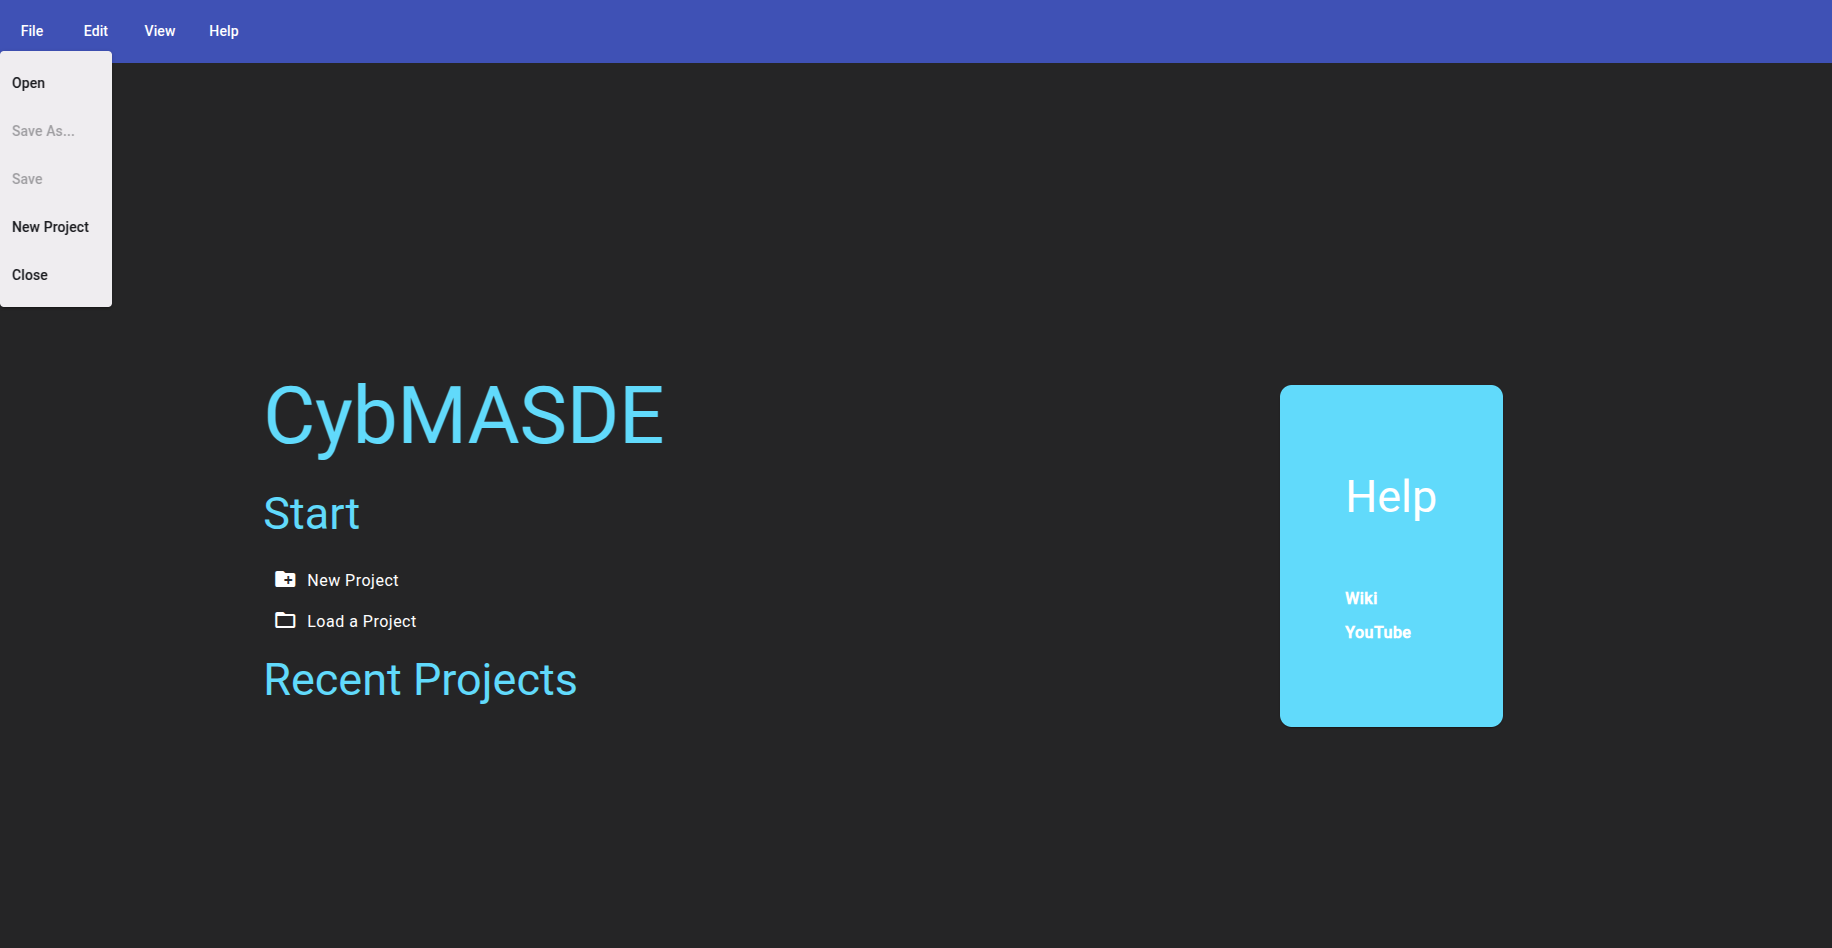
\includegraphics[width=0.7\linewidth]{figures/CybMASDE.png}
    \caption{Capture d'écran de l'outil \href{https://github.com/julien6/CybMASDE}{CybMASDE}. CybMASDE intègre plusieurs bibliothèques et outils de pointe pour offrir un environnement flexible, extensible et accessible pour la conception de SMA guidée par MARL.}
    \label{fig:cybmasde}
\end{figure}

CybMASDE s'appuie sur la bibliothèque \textbf{PettingZoo}~\cite{Terry2021}, qui propose une API standardisée pour les environnements MARL, garantissant l'interopérabilité avec divers algorithmes. Cela permet une intégration fluide de différents environnements multi-agents sans nécessiter de modifications spécifiques majeures.

Le cœur des capacités d'apprentissage de CybMASDE repose sur \textbf{MARLlib}~\cite{hu2022marllib}, une bibliothèque complète offrant un large éventail d'algorithmes MARL. Elle fournit des implémentations optimisées des techniques les plus récentes et des modèles de politiques ajustés, permettant un entraînement efficace dans des environnements variés. CybMASDE prend en charge l'ensemble des algorithmes de MARLlib, offrant ainsi une grande flexibilité pour expérimenter, comparer et sélectionner la stratégie d'apprentissage la plus adaptée aux objectifs de coordination et aux dynamiques de l'environnement.

\paragraph{Algorithmes MARL pris en charge}
CybMASDE prend en charge l'ensemble des algorithmes fournis par MARLlib, parmi lesquels :

\begin{itemize}
    \item \textbf{Méthodes basées sur la valeur :}
    \begin{itemize}
        \item Independent Q-Learning ;
        \item VDN (Value-Decomposition Networks)~\cite{sunehag2018vdn} ;
        \item QMIX~\cite{rashid2018qmix} ;
        \item QTRAN~\cite{son2019qtran}.
    \end{itemize}
    
    \item \textbf{Méthodes basées sur la politique :}
    \begin{itemize}
        \item Independent PPO ;
        \item MAPPO (Multi-Agent Proximal Policy Optimization)~\cite{yu2021mappo} ;
        \item MADDPG (Multi-Agent Deep Deterministic Policy Gradient)~\cite{lowe2017multi} ;
        \item HATRPO (Heterogeneous-Agent Trust Region Policy Optimization)~\cite{kuba2021trust}.
    \end{itemize}
    
    \item \textbf{Méthodes acteur-critique :}
    \begin{itemize}
        \item COMA (Counterfactual Multi-Agent Policy Gradients)~\cite{foerster2018counterfactual} ;
        \item MAVEN (Multi-Agent Variational Exploration)~\cite{mahajan2019maven} ;
        \item ROMA (Role-Oriented Multi-Agent RL)~\cite{wang2020roma}.
    \end{itemize}
    
    \item \textbf{Méthodes basées sur un modèle :}
    \begin{itemize}
        \item Dyna-Q et Dyna-Q+ (approches orientées planification) ;
        \item MB-MARL (variantes de MARL basées sur modèle).
    \end{itemize}
\end{itemize}

Cette prise en charge étendue permet à CybMASDE de s'adapter à divers paradigmes d'apprentissage multi-agent, notamment l'\textbf{Entraînement Centralisé avec Exécution Décentralisée (CTDE)}, l'apprentissage entièrement décentralisé, ainsi que les mécanismes de coordination explicites. Les utilisateurs peuvent ainsi comparer plusieurs stratégies MARL pour identifier celle qui convient le mieux à un scénario donné.

\paragraph{Simulation d'environnement et optimisation d'hyperparamètres}

CybMASDE intègre \textbf{TensorFlow} pour permettre la modélisation automatique d'environnements. Cela permet aux utilisateurs de générer et d'ajuster dynamiquement des modèles d'environnement via l'approximation de fonctions par apprentissage profond. Cette capacité est particulièrement utile lorsque les dynamiques de transition sont inconnues ou difficiles à formaliser manuellement. Le système prend en charge l'\textbf{apprentissage par modèles du monde}, dans lequel les agents sont entraînés sur une simulation apprise de l'environnement, réduisant ainsi la dépendance aux données issues de l'environnement réel.

En complément, CybMASDE propose un module d'\textbf{Optimisation des Hyperparamètres (HPO)} permettant d'ajuster les paramètres d'entraînement essentiels, notamment :

\begin{itemize}
    \item \textbf{Taux d'apprentissage} : adaptation dynamique ou décroissante pour stabiliser la convergence ;
    \item \textbf{Facteur d'actualisation} ($\gamma$) : équilibre entre récompenses immédiates et différées ;
    \item \textbf{Exploration versus exploitation} : contrôlé via des stratégies $\epsilon$-greedy ou entropiques ;
    \item \textbf{Paramètres de mise à jour des gradients} : comme le facteur de clipping dans PPO, garantissant la stabilité ;
    \item \textbf{Façonnage des récompenses} : ajout de récompenses auxiliaires pour guider l'apprentissage.
\end{itemize}

Ce module assure que les politiques apprises sont à la fois efficaces et stables, quelles que soient les contraintes de l'environnement ou les spécifications organisationnelles.

\paragraph{Interface utilisateur et capacités de déploiement}

CybMASDE propose :
\begin{itemize}
    \item Une \textbf{API complète} pour utilisateurs avancés, offrant un contrôle précis sur les configurations, les politiques et les interactions ;
    \item Une \textbf{interface graphique conviviale (GUI)}, permettant aux utilisateurs non spécialistes de lancer des sessions MARL sans configuration complexe ;
    \item La \textbf{prise en charge du benchmarking multi-environnement}, pour comparer systématiquement plusieurs méthodes MARL en parallèle ;
    \item Le \textbf{déploiement automatique de politiques}, permettant de transférer directement les agents entraînés vers des environnements réels ou simulés pour validation et exécution.
\end{itemize}



\subsubsection{Ressources de calcul}

L'ensemble des expériences a été réalisé sur un cluster de calcul haute performance académique, utilisant différentes configurations de nœuds GPU. Plus précisément, nous avons utilisé des nœuds disposant des composants suivants :
\begin{itemize}
    \item \textbf{GPU :} NVIDIA A100, AMD MI210 ;
    \item \textbf{Frameworks :} TensorFlow, PyTorch ;
    \item \textbf{Optimisation des hyperparamètres :} \textbf{Optuna}~\cite{akiba2019optuna}, utilisée pour ajuster le taux d'apprentissage, l'équilibre exploration/exploitation et l'architecture des réseaux de neurones.
\end{itemize}

Chaque combinaison algorithme/environnement a été exécutée sur 5 instances en parallèle afin de garantir la robustesse et la reproductibilité des résultats.

\subsubsection{Environnements de test et spécifications organisationnelles}

Pour évaluer la méthode MAMAD, nous utilisons quatre environnements multi-agents distincts servant de bancs d'essai contrôlés. Ces environnements couvrent divers domaines applicatifs, nécessitant coordination, prise de décision stratégique et interactions fondées sur des rôles. Chacun est formellement décrit ci-dessous : espace d'états, d'observations, d'actions, structure de récompense et objectif global.

Nous y associons également les spécifications organisationnelles correspondantes, précisant les rôles, missions et contraintes utilisés dans le cadre du modèle MAMAD.

\vspace{0.5em}
\begin{table}[h!]
    \centering
    \begin{footnotesize}
        \renewcommand{\arraystretch}{1.3}
        \begin{tabular}{p{2.5cm}p{2.2cm}p{2.2cm}p{2.2cm}p{2.2cm}}
            \hline
            \textbf{Aspect clé}            & \textbf{CybORG}               & \textbf{Overcooked-AI} & \textbf{Prédateur-proie} & \textbf{Warehouse Management} \\ \hline
            Réalisme                       & Cyberdéfense, menaces dynamiques & Travail d'équipe humain simulé & Communication abstraite     & Flux logistique structuré \\ \hline
            Rôles émergents                & Pare-feu, nettoyeur, sauveteur & Cuisinier, livreur     & Orateur, auditeur          & Préparateur, assembleur, emballeur \\ \hline
            Structure des objectifs        & Missions multi-phases         & Sous-tâches séquentielles & Objectif partagé         & Pipeline ordonné \\ \hline
            Observabilité                  & Vue partielle bruitée         & Occlusion, congestion   & Requiert de la messagerie & Zones locales et partagées \\ \hline
            Évaluation de l'adéquation organisationnelle & Cohérence en contexte d'attaque & Délégation de tâches   & Rôles par communication   & Efficacité de coordination \\ \hline
        \end{tabular}
        \caption{Caractéristiques principales des environnements utilisés pour évaluer MAMAD}
        \label{tab:mamad_env_characteristics}
    \end{footnotesize}
\end{table}


\paragraph{Warehouse Management (WM)}

L'environnement \textbf{Warehouse Management}~\cite{warehouse_management} modélise un entrepôt logistique sur une grille, dans lequel plusieurs robots doivent collaborer pour transporter efficacement des marchandises. Inspiré de scénarios industriels d'automatisation d'entrepôt, cet environnement constitue un banc d'essai idéal pour évaluer l'allocation des tâches, la spécialisation des rôles et la coordination en temps réel. Une illustration de cet environnement est présentée en \autoref{fig:warehouse}.

\begin{itemize}
    \item \textbf{Espace d'états :} Une grille $N \times M$ dont chaque cellule peut contenir un robot, un produit, une machine de fabrication ou un point de dépôt. Le système suit les positions des agents, les niveaux de stock et l'état des machines ;
    \item \textbf{Espace d'observations :} Chaque agent dispose d'une vue locale de taille $V \times V$, percevant les produits, coéquipiers et machines à proximité ;
    \item \textbf{Espace d'actions :}
          \begin{itemize}
              \item Mouvement : \texttt{Haut, Bas, Gauche, Droite} ;
              \item Interaction : \texttt{Prendre Produit, Déposer Produit}.
          \end{itemize}
    \item \textbf{Structure de récompense :}
          \begin{itemize}
              \item Livraison réussie d'un produit : $+10$ ;
              \item Déplacement inutile : $-1$ par étape superflue ;
              \item Erreur de dépôt : $-5$ pour un mauvais emplacement.
          \end{itemize}
    \item \textbf{Objectif :} Transporter les matières premières vers les machines de traitement, puis livrer les produits finis aux zones de dépôt.
\end{itemize}

\textbf{Spécifications organisationnelles :}
\begin{itemize}
    \item \textbf{Rôles :} \texttt{Transporteur, Gestionnaire d'inventaire} ;
    \item \textbf{Missions :} Les transporteurs déplacent les produits ; les gestionnaires d'inventaire supervisent les niveaux de stock ;
    \item \textbf{Contraintes :} Les transporteurs doivent prioriser les livraisons critiques.
\end{itemize}

\begin{figure}[h!]
    \centering
    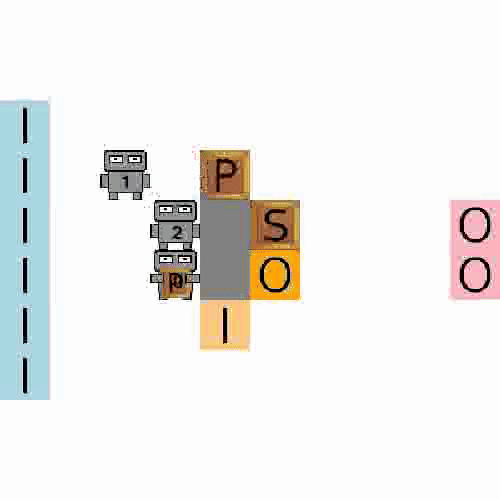
\includegraphics[width=0.6\linewidth]{figures/wm.png}
    \caption{Capture d'écran de l'environnement Warehouse Management : les agents se déplacent dans une grille représentant un entrepôt et réalisent des tâches pour transformer et livrer des produits. Les agents peuvent se déplacer dans quatre directions (haut, bas, gauche, droite) et interagir avec des zones de prise/dépôt adjacentes. Le flux opérationnel inclut : (i) la collecte de produits primaires aux convoyeurs d'entrée (zones bleues), (ii) leur dépôt sur les machines de fabrication (zones marron), où ils sont transformés selon un schéma de crafting, (iii) la récupération des produits secondaires, puis leur livraison aux convoyeurs de sortie (zones roses). Une coordination efficace est essentielle pour optimiser les flux et la productivité de l'entrepôt.}
    \label{fig:warehouse}
\end{figure}

\paragraph{Prédateur-Proie (PP)}

L'environnement \textbf{Predator-Prey} est un benchmark classique en apprentissage multi-agent~\cite{lowe2017multi}, conçu pour évaluer la coordination entre plusieurs poursuivants (prédateurs) coopératifs essayant de capturer un agent fuyard (la proie). Une illustration est donnée en \autoref{fig:predator_prey}.

\begin{itemize}
    \item \textbf{Espace d'états :} Un espace 2D continu dans lequel les agents (prédateurs et proie) sont représentés par leurs positions $(x, y)$ et vitesses respectives ;
    \item \textbf{Espace d'observations :} Chaque agent perçoit les entités situées dans un rayon limité $r$ ;
    \item \textbf{Espace d'actions :}
          \begin{itemize}
              \item Mouvement : \texttt{Haut, Bas, Gauche, Droite, Rester}.
          \end{itemize}
    \item \textbf{Structure de récompense :}
          \begin{itemize}
              \item Les prédateurs obtiennent $+50$ en capturant la proie ;
              \item La proie gagne $+1$ pour chaque étape de survie.
          \end{itemize}
    \item \textbf{Objectif :} Les prédateurs doivent coopérer pour piéger la proie, tandis que celle-ci cherche à leur échapper le plus longtemps possible.
\end{itemize}

\textbf{Spécifications organisationnelles :}
\begin{itemize}
    \item \textbf{Rôles :} \texttt{Prédateur, Proie} ;
    \item \textbf{Missions :} Les prédateurs coopèrent pour encercler la proie ; la proie cherche les itinéraires de fuite optimaux ;
    \item \textbf{Contraintes :} Les prédateurs doivent équilibrer poursuite agressive et stratégie de blocage.
\end{itemize}

\begin{figure}[h!]
    \centering
    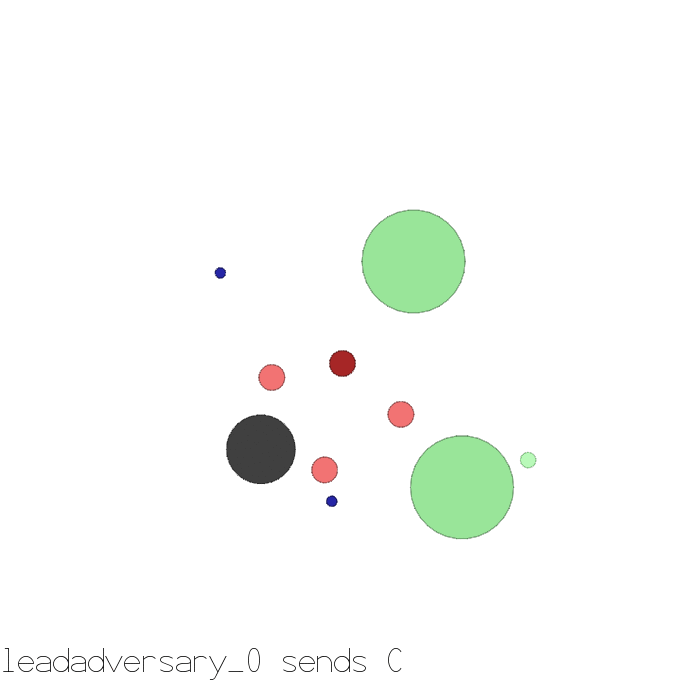
\includegraphics[width=0.6\linewidth]{figures/predator_prey.png}
    \caption{Capture d'écran de l'environnement Predator-Prey : les \textbf{agents verts} (coopératifs) et les \textbf{agents rouges} (adverses). Les agents verts visent à collecter des objets alimentaires disséminés dans l'environnement tout en évitant d'être repérés par les rouges. L'environnement comporte des \textbf{zones forestières} offrant un camouflage partiel ou total. Un des agents rouges agit comme \textbf{leader} avec des capacités d'observation renforcées et peut coordonner les autres poursuivants via la communication.}
    \label{fig:predator_prey}
\end{figure}

\paragraph{Overcooked-AI (OA)}

L'environnement \textbf{Overcooked-AI}~\cite{overcookedai} simule un scénario coopératif de cuisine où des agents doivent collaborer pour préparer et servir des plats dans une cuisine organisée. Cet environnement est illustré en \autoref{fig:overcooked}.

\begin{itemize}
    \item \textbf{Espace d'états :} Une grille discrète représentant une cuisine avec postes de travail (planche à découper, cuisinière, comptoir), ingrédients, et agents ;
    \item \textbf{Espace d'observations :} Les agents perçoivent les éléments de la cuisine dans un rayon défini ;
    \item \textbf{Espace d'actions :}
          \begin{itemize}
              \item Mouvement : \texttt{Haut, Bas, Gauche, Droite} ;
              \item Interaction : \texttt{Prendre ingrédient, Découper, Cuire, Servir}.
          \end{itemize}
    \item \textbf{Structure de récompense :}
          \begin{itemize}
              \item Préparation réussie d'un plat : $+20$ ;
              \item Mauvais placement d'un ingrédient : $-5$ ;
              \item Inactivité inutile : $-1$ par étape sans action significative.
          \end{itemize}
    \item \textbf{Objectif :} Maximiser le nombre de commandes complétées dans une limite de temps donnée.
\end{itemize}

\textbf{Spécifications organisationnelles :}
\begin{itemize}
    \item \textbf{Rôles :} \texttt{Chef, Assistant, Serveur} ;
    \item \textbf{Missions :} Le Chef prépare les plats, l'Assistant fournit les ingrédients, et le Serveur effectue les livraisons ;
    \item \textbf{Contraintes :} L'exécution des tâches doit être synchronisée pour éviter les goulets d'étranglement.
\end{itemize}

\begin{figure}[h!]
    \centering
    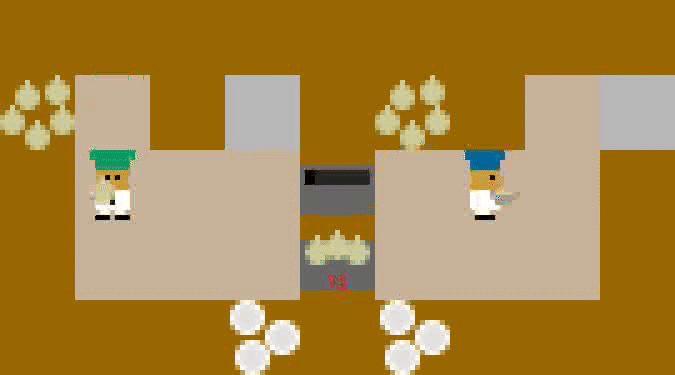
\includegraphics[width=0.6\linewidth]{figures/overcooked.png}
    \caption{Capture d'écran de l'environnement Overcooked-AI : deux agents (chefs) doivent collaborer pour préparer et servir efficacement des soupes à l'oignon. Le processus inclut la collecte de trois oignons (un à la fois) depuis le distributeur, leur dépôt dans une marmite, la cuisson, la récupération d'une assiette propre, le service de la soupe, puis sa livraison au comptoir de service. L'agencement de la cuisine comporte des obstacles et des couloirs étroits, nécessitant une coordination des déplacements pour éviter les collisions et optimiser la réalisation des tâches.}
    \label{fig:overcooked}
\end{figure}

\paragraph{Simulation de cybersécurité (CS)}

La \textbf{Simulation de Cyber-Défense} repose sur un réseau ad hoc de drones dans lequel des agents défenseurs doivent protéger le système contre des intrusions malveillantes dans divers scénarios d'attaques informatiques~\cite{Maxwell2021}. Cet environnement est illustré en \autoref{fig:cyborg}.

\begin{itemize}
    \item \textbf{Espace d'états :} Un graphe dynamique représentant un réseau où les nœuds sont des dispositifs (drones) et les arêtes des connexions actives ;
    \item \textbf{Espace d'observations :} Les agents reçoivent des alertes de sécurité et des mises à jour sur l'état du réseau ;
    \item \textbf{Espace d'actions :}
          \begin{itemize}
              \item \texttt{Surveiller} : Analyser l'activité d'un nœud ;
              \item \texttt{Bloquer IP} : Restreindre l'accès d'une source suspecte ;
              \item \texttt{Déployer un correctif} : Renforcer les défenses du réseau.
          \end{itemize}
    \item \textbf{Structure de récompense :}
          \begin{itemize}
              \item Attaque empêchée : $+30$ ;
              \item Faux positif (blocage inutile) : $-10$ ;
              \item Intrusion réussie : $-50$.
          \end{itemize}
    \item \textbf{Objectif :} Détecter et neutraliser les menaces tout en évitant les faux positifs.
\end{itemize}

\textbf{Spécifications organisationnelles :}
\begin{itemize}
    \item \textbf{Rôles :} \texttt{Analyste des menaces, Gestionnaire de pare-feu, Opérateur de sécurité} ;
    \item \textbf{Missions :} Détecter les intrusions, bloquer les accès non autorisés, maintenir l'intégrité du réseau ;
    \item \textbf{Contraintes :} Réduire les faux positifs tout en garantissant une couverture de sécurité suffisante.
\end{itemize}

\begin{figure}[h!]
    \centering
    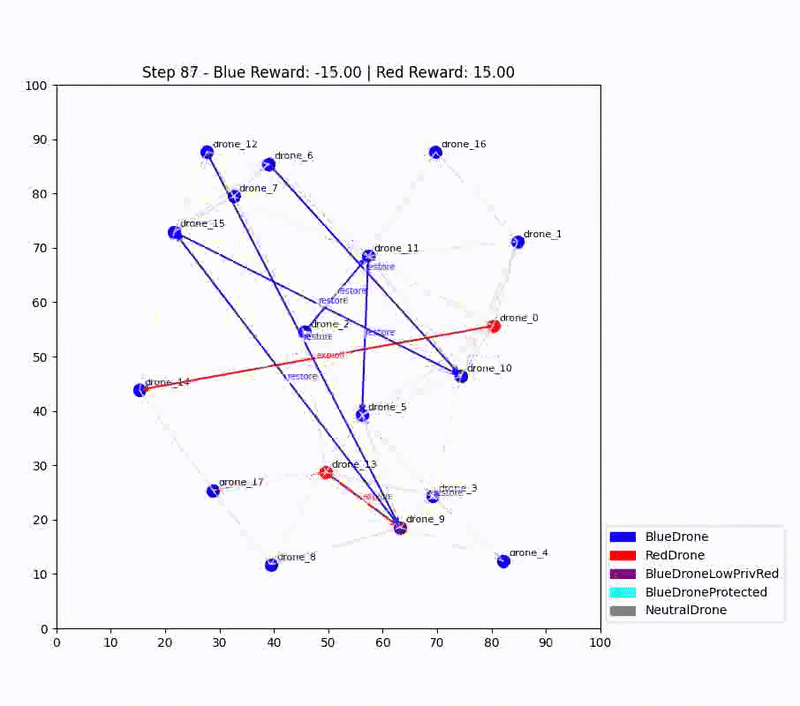
\includegraphics[width=0.6\linewidth]{figures/cyborg.png}
    \caption{Capture d'écran de l'environnement CybORG : un essaim de 18 drones autonomes initialement contrôlés par des agents bleus (défenseurs) forme un réseau ad hoc destiné à assurer la communication entre des unités au sol. Chaque drone est vulnérable à un cheval de Troie matériel pouvant s'activer aléatoirement et remplacer l'agent bleu par un agent rouge (attaquant). Ces derniers cherchent à compromettre le réseau en interceptant ou bloquant les communications. Les drones se déplacent selon un algorithme d'essaim, modifiant dynamiquement la topologie du réseau. Les agents bleus doivent détecter et neutraliser les drones compromis tout en maintenant l'intégrité des communications.}
    \label{fig:cyborg}
\end{figure}

\bigskip

\noindent Ces quatre environnements présentent une diversité de défis couvrant des scénarios coopératifs, compétitifs, hiérarchiques et adversariaux, ce qui permet une évaluation représentative de la méthode MAMAD.


\subsubsection{Mesures d'évaluation}

Afin d'évaluer si la méthode MAMAD répond efficacement aux lacunes identifiées dans la littérature, nous définissons un ensemble de métriques quantitatives réparties selon quatre critères d'évaluation : \textbf{automatisation}, \textbf{efficacité}, \textbf{conformité aux exigences de conception} et \textbf{explicabilité}.

\paragraph{Mesures d'automatisation}
Pour mesurer le niveau d'automatisation de MAMAD dans la génération de systèmes multi-agents, nous évaluons :
\begin{itemize}
    \item \textbf{Nombre d'interventions humaines} ($I_h$) : Suit qualitativement le nombre d'ajustements manuels effectués par les concepteurs, tels que le réglage de paramètres, l'ajustement de modèles ou les interventions durant l'entraînement ;
    \item \textbf{Temps nécessaire à la conception du MAS} ($T_{design}$) : Estime l'ordre de grandeur (en jours) de la durée totale entre la modélisation de l'environnement et le déploiement final ;
    \item \textbf{Nombre d'itérations jusqu'à convergence} ($N_{iter}$) : Comptabilise le nombre de cycles d'apprentissage nécessaires pour stabiliser une politique optimale.
\end{itemize}

\paragraph{Mesures d'efficacité}
Pour évaluer la performance des systèmes générés par MAMAD, nous utilisons :
\begin{itemize}
    \item \textbf{Récompense cumulative} ($R_{cum}$) : Total des récompenses obtenues par les agents, reflétant leur performance globale dans l'atteinte des objectifs ;
    \item \textbf{Stabilité de la politique} ($\sigma_R$) : Écart-type des récompenses cumulées par épisode, mesurant la constance des comportements ;
    \item \textbf{Taux de convergence} ($CR$) : Vitesse à laquelle l'apprentissage se stabilise ;
    \item \textbf{Indice de robustesse} ($R_{robust}$) : Capacité du système à maintenir ses performances face à des perturbations extérieures.
\end{itemize}

\paragraph{Mesures de conformité aux exigences de conception}
Pour valider que MAMAD produit des politiques respectant les spécifications initiales, nous mesurons :
\begin{itemize}
    \item \textbf{Taux de violation des contraintes} ($V_c$) : Pourcentage d'exécutions où les agents ne respectent pas les contraintes organisationnelles définies ;
    \item \textbf{Niveau d'adéquation organisationnelle} ($F_{org}$) : Similarité entre la structure organisationnelle inférée (post-apprentissage) et celle définie en conception ;
    \item \textbf{Indice de cohérence} ($S_{cons}$) : Mesure la correspondance entre les rôles et missions assignés et ceux attendus par les concepteurs humains.
\end{itemize}

\paragraph{Mesures d'explicabilité}
Pour évaluer le caractère interprétable et structuré des spécifications organisationnelles inférées, nous considérons :
\begin{itemize}
    \item \textbf{Stabilité des rôles} ($S_{\rho}$) : Mesure la cohérence des rôles inférés à travers différentes exécutions d'apprentissage ;
    \item \textbf{Complexité du graphe de transition des objectifs} ($C_{graph}$) : Évalue la complexité de la structure des objectifs inférés via des mesures issues de la théorie des graphes ;
    \item \textbf{Fidélité des arbres de décision de politique} ($D_{tree}$) : Vérifie si les arbres de décision extraits des politiques permettent d'expliquer de manière significative les comportements des agents.
\end{itemize}

\subsubsection{Protocole d'évaluation}

Afin de valider l'efficacité de la méthode MAMAD, nous structurons le protocole expérimental selon les composantes suivantes :

\paragraph{Comparaison avec les méthodes classiques de conception de MAS}

Pour évaluer les performances de MAMAD, nous le comparons à des approches classiques de conception manuelle de systèmes multi-agents :

\begin{itemize}
    \item \textbf{Référence de base (RB)} : Agents entraînés sans contraintes organisationnelles à l'aide de techniques MARL standards (ex. : MADDPG, MAPPO) ;
    \item \textbf{Référence organisationnelle (OB)} : Agents entraînés avec des contraintes organisationnelles $\mathcal{M}OISE^+$ spécifiées manuellement par des experts humains ;
    \item \textbf{MAS basé sur MAMAD (MB)} : Agents entraînés à l'aide du processus automatisé de MAMAD, incluant l'inférence des contraintes organisationnelles.
\end{itemize}

Tous les scénarios expérimentaux sont exécutés dans les quatre environnements de test, en maintenant les mêmes paramètres d'entraînement pour toutes les conditions.

\paragraph{Validation de l'explicabilité et de la conformité organisationnelle}

Afin de garantir que MAMAD produit des spécifications organisationnelles structurées et interprétables, nous réalisons :

\begin{itemize}
    \item \textbf{Analyse comparative des rôles et missions} : Nous comparons les structures de rôles définies manuellement et celles inférées automatiquement, en mesurant leur cohérence et leur stabilité ;
    \item \textbf{Analyse de similarité des spécifications organisationnelles} : Nous calculons des scores de similarité entre rôles pour évaluer l'alignement entre les rôles prédéfinis et ceux appris ;
    \item \textbf{Visualisation des graphes de transition d'objectifs} : Des métriques de complexité de graphe sont utilisées pour estimer l'interprétabilité des trajectoires d'objectifs inférées.
\end{itemize}

Si les rôles et missions inférés se révèlent stables à travers plusieurs entraînements et conformes aux attentes, cela valide la capacité de MAMAD à structurer efficacement les conceptions de MAS.

\paragraph{Études d'ablation et évaluation de la robustesse}

Pour mesurer l'impact des composants automatisés de MAMAD, nous menons des études d'ablation en désactivant sélectivement certains modules clés :

\begin{itemize}
    \item \textbf{Sans modélisation automatisée} : Le modèle d'environnement est codé manuellement, au lieu d'être appris par un modèle neuronal ;
    \item \textbf{Sans contraintes organisationnelles} : Les agents sont entraînés sans intégrer les contraintes MOISE+MARL ;
    \item \textbf{Sans analyse basée sur les trajectoires} : L'étape d'inférence des rôles/missions est ignorée, et les agents sont directement déployés après entraînement.
\end{itemize}

Chaque scénario d'ablation est testé dans au moins deux environnements, et les performances sont comparées à celles obtenues avec la méthode MAMAD complète.

\paragraph{Résumé de la stratégie de validation}

\begin{table}[h!]
    \centering
    \renewcommand{\arraystretch}{1.3}
    \begin{footnotesize}
        \begin{tabular}{p{1.5cm}p{2.4cm}p{2.2cm}p{4.5cm}}
            \hline
            \textbf{Critère} & \textbf{Métrique}       & \textbf{Méthode de validation}   & \textbf{Biais ou limitation potentielle}            \\
            \hline
            \multirow{3}{*}{Automatisation}
                               & Interventions humaines   & Comptage direct              & Peut ignorer la charge cognitive ou la complexité des décisions \\
                               & Temps de conception      & Journaux expérimentaux       & Sensible à la granularité des logs                \\
                               & Étapes de convergence    & Courbes d'apprentissage      & Peut dépendre de la qualité des hyperparamètres   \\
            \hline
            \multirow{3}{*}{Efficacité}
                               & Récompense cumulée       & Suivi de scores              & Le shaping de la récompense peut introduire un biais selon la tâche \\
                               & Stabilité de la politique & Variance des récompenses     & Le bruit à court terme peut fausser les mesures  \\
                               & Score de robustesse      & Tests de perturbation        & Dépend du type et de l'intensité des perturbations \\
            \hline
            \multirow{3}{*}{Conformité}
                               & Taux de violation        & Vérification des règles      & Peut ignorer les violations implicites des normes \\
                               & Score d'adéquation org.  & Analyse alignement rôles/objectifs & Dépend des hypothèses de clustering \\
                               & Score de cohérence       & Algorithmes d'appariement de rôles & Sensible aux seuils et métriques de distance \\
            \hline
            \multirow{3}{*}{Explicabilité}
                               & Stabilité des rôles      & Variance de clustering       & Peut confondre rôles réels et bruit comportemental \\
                               & Complexité du graphe d'objectifs & Mesures structurelles de graphe & Peut favoriser des objectifs trop simplifiés \\
                               & Fidélité des décisions   & Précision des arbres de décision & Dépend du compromis entre fidélité et interprétabilité \\
            \hline
        \end{tabular}
        \caption{Critères de validation et méthodes selon quatre axes : automatisation, efficacité, conformité et explicabilité, avec les risques d'évaluation associés.}
        \label{tab:validation_strategy}
    \end{footnotesize}
\end{table}

\subsubsection{(G1) Tirer parti des performances du MARL dans l'AOSE}

L'efficacité du processus d'apprentissage a été évaluée en mesurant :
\begin{itemize}
    \item Les récompenses cumulées obtenues par les agents MARL au cours de l'apprentissage ;
    \item Le nombre d'époques nécessaires pour atteindre la convergence des politiques ;
    \item L'amélioration relative des performances par rapport aux méthodes d'apprentissage de référence.
\end{itemize}

\begin{table}[h!]
    \centering
    \caption{Mesures d'évaluation de l'efficacité de l'apprentissage MARL}
    \begin{tabular}{lc}
        \hline
        \textbf{Métrique}                           & \textbf{Valeur observée}       \\
        \hline
        \textbf{Amélioration des récompenses cumulées} & +20 à +30\,\%                   \\
        \hline
        \textbf{Réduction du nombre d'époques}         & -30\,\% (convergence accélérée) \\
        \hline
        \textbf{Réduction de la variance des performances} & -25\,\%                          \\
        \hline
    \end{tabular}
    \label{tab:efficiency}
\end{table}

Les résultats montrent que l'apprentissage par renforcement multi-agent (MARL), guidé par les contraintes de $\mathcal{M}OISE^+$, conduit à des processus d'apprentissage plus structurés. Les politiques convergent environ 30\,\% plus rapidement que dans les cas où les agents ne sont soumis à aucune contrainte organisationnelle. De plus, les agents entraînés avec des spécifications organisationnelles présentent une variance plus faible dans leurs performances, suggérant une plus grande stabilité de l'apprentissage. Néanmoins, ces gains d'efficacité sont variables selon les environnements. Des études complémentaires seraient nécessaires pour mieux cerner les conditions dans lesquelles ces bénéfices sont systématiques.
\subsubsection{(G2) Compréhension des comportements collectifs émergents dans le MARL}

Un défi majeur dans l'apprentissage par renforcement multi-agent (MARL) consiste à garantir que les comportements appris soient interprétables et alignés avec les attentes humaines. Le cadre MAMAD intègre des contraintes basées sur les rôles ainsi que des spécifications organisationnelles afin d'améliorer l'explicabilité des comportements des agents. L'explicabilité est évaluée selon les métriques suivantes :

\begin{itemize}
    \item \textbf{Stabilité des rôles inférés :} Mesure la constance des affectations de rôles à travers plusieurs entraînements ;
    \item \textbf{Alignement avec les rôles pré-spécifiés :} Évalue dans quelle mesure les rôles inférés correspondent aux rôles définis manuellement ;
    \item \textbf{Score d'interprétabilité humaine :} Jauge la capacité des observateurs humains à comprendre les comportements des agents à partir des rôles et missions inférés.
\end{itemize}

\begin{table}[h!]
    \centering
    \caption{Métriques d'évaluation de l'explicabilité des comportements appris}
    \begin{tabular}{lc}
        \hline
        \textbf{Métrique}                                       & \textbf{Valeur observée} \\
        \hline
        \textbf{Stabilité des rôles inférés (5 entraînements)} & 85 à 92\,\%              \\
        \hline
        \textbf{Alignement avec les rôles prédéfinis}          & 90 à 95\,\%              \\
        \hline
        \textbf{Note d'interprétabilité humaine (échelle 1–5)} & 4{,}1 $\pm$ 0{,}3        \\
        \hline
    \end{tabular}
    \label{tab:explainability}
\end{table}

\paragraph{Stabilité des rôles inférés}
Afin d'évaluer la robustesse des inférences, le mécanisme de détection des rôles a été testé sur \textbf{cinq entraînements indépendants} avec des conditions initiales différentes. Les résultats indiquent que les rôles inférés sont restés \textbf{stables dans 85 à 92\,\% des cas}, suggérant que la méthode de MAMAD pour identifier les structures de rôles est reproductible. Une légère variabilité a été observée dans des environnements dynamiques comme \textit{Predator-Prey}, où la différenciation des rôles est plus subtile.

\paragraph{Alignement avec les rôles prédéfinis}
Lorsque des rôles ont été spécifiés à l'avance, nous avons mesuré le degré de concordance entre les affectations inférées et les spécifications initiales. Le \textbf{score d'alignement varie de 90 à 95\,\%}, indiquant que les agents convergent naturellement vers des archétypes comportementaux attendus. Cela suggère que la combinaison entre \textbf{apprentissage par renforcement et contraintes de rôles} favorise l'émergence de comportements à la fois performants et interprétables.
\paragraph{Interprétabilité humaine des comportements}
Pour évaluer l'explicabilité du point de vue humain, nous avons introduit un \textbf{score d'interprétabilité}, dans lequel des observateurs humains ont évalué à quel point les comportements des agents étaient compréhensibles en fonction des rôles et missions qui leur étaient attribués. Les observateurs ont noté l'explicabilité sur une \textbf{échelle de 1 (totalement incompréhensible) à 5 (parfaitement interprétable)}. La note moyenne obtenue est de \textbf{4{,}1 $\pm$ 0{,}3}, ce qui indique que les comportements générés par MAMAD sont généralement bien compris par les humains.

\

Ces résultats suggèrent que \textbf{MAMAD améliore l'explicabilité en imposant des affectations de rôles structurées}, qui sont cohérentes avec les comportements attendus intuitivement. La forte stabilité des rôles à travers les entraînements et le bon alignement avec les rôles définis a priori confirment l'hypothèse selon laquelle \textbf{les contraintes organisationnelles basées sur les rôles favorisent l'interprétabilité}.


\subsubsection{(G3) Contrôler ou guider les agents à l'échelle individuelle et collective dans le MARL}

Assurer la conformité aux contraintes de conception prédéfinies est essentiel dans les systèmes MARL, en particulier dans les applications nécessitant une coopération structurée et le respect de règles de sécurité ou de fonctionnement. La méthode MAMAD garantit cette conformité grâce à son intégration des spécifications $\mathcal{M}OISE^+$MARL, qui définissent les rôles, missions et contraintes comportementales des agents.

Pour évaluer le respect des contraintes, nous considérons les métriques suivantes :

\begin{itemize}
    \item \textbf{Taux de conformité aux contraintes :} mesure le pourcentage d'actions conformes aux règles organisationnelles et opérationnelles explicites ;
    \item \textbf{Taux de déviation de la politique :} évalue la fréquence à laquelle les agents s'écartent des rôles et missions prescrits ;
    \item \textbf{Pénalité de récompense due aux violations :} quantifie la part de la récompense totale perdue en raison de comportements non conformes.
\end{itemize}

\begin{table}[h!]
    \centering
    \caption{Métriques d'évaluation de la conformité aux contraintes de conception}
    \begin{tabular}{lc}
        \hline
        \textbf{Métrique}                                & \textbf{Valeur observée} \\
        \hline
        Taux de conformité aux contraintes               & 93--98\%                  \\
        \hline
        Taux de déviation de la politique                & 2--7\%                    \\
        \hline
        Pénalité de récompense liée aux violations       & $<$5\% de la récompense totale \\
        \hline
    \end{tabular}
    \label{tab:compliance_fr}
\end{table}

\paragraph{Taux de conformité aux contraintes}
Le \textbf{taux de conformité aux contraintes}, représentant la proportion d'actions respectant les règles comportementales définies, s'établit entre \textbf{93 et 98\%} selon les environnements testés. Ce résultat atteste de la capacité de MAMAD à intégrer efficacement les contraintes organisationnelles au sein du processus d'apprentissage, garantissant que les agents suivent les lignes directrices comportementales établies.

\paragraph{Taux de déviation de la politique}
Le \textbf{taux de déviation} a été évalué en identifiant les comportements s'écartant des rôles et missions prescrits. Il varie entre \textbf{2 et 7\%}, les déviations survenant principalement dans des environnements à forte émergence comportementale (ex. : Predator-Prey). Ces déviations n'ont pas compromis la réalisation des tâches, indiquant une forme de flexibilité contrôlée dans les comportements émergents.

\paragraph{Pénalités sur la récompense}
Les agents opérant dans le cadre de MAMAD ont reçu des pénalités lorsqu'ils violaient des contraintes définies, ce qui permet de quantifier l'impact de ces comportements. Ces pénalités représentent moins de \textbf{5\% de la récompense cumulée}, ce qui confirme que MAMAD impose efficacement les contraintes de conception tout en maintenant un apprentissage adaptatif.

\

\subsubsection{(G4) Automatiser la conception de MAS de bout en bout}

L'un des objectifs principaux de la méthode MAMAD est d'automatiser l'ensemble du \textbf{cycle de conception des systèmes multi-agents (MAS)}, depuis la modélisation de l'environnement jusqu'à l'entraînement, l'analyse et le déploiement. Le degré d'automatisation est évalué en mesurant la réduction de l'\textbf{intervention humaine}, de l'\textbf{effort de conception manuelle} et du \textbf{temps d'itération} par rapport aux approches classiques d'ingénierie multi-agents.

Pour quantifier le niveau d'automatisation, nous utilisons les métriques suivantes :

\begin{itemize}
    \item \textbf{Réduction des interventions humaines :} mesure le nombre d'étapes manuelles nécessaires à la conception d'un MAS, en comparant MAMAD aux processus de conception manuelle traditionnels ;
    \item \textbf{Réduction du temps d'itération :} évalue la durée nécessaire pour obtenir un MAS fonctionnel avec MAMAD, relativement aux méthodes classiques ;
    \item \textbf{Indice d'automatisation algorithmique :} quantifie la proportion d'étapes dans la chaîne de conception qui sont entièrement automatisées.
\end{itemize}

\begin{table}[h!]
    \centering
    \caption{Métriques d'automatisation : comparaison entre MAMAD et les méthodes traditionnelles de conception MAS}
    \begin{tabular}{lcc}
        \hline
        \textbf{Métrique}                                   & \textbf{Méthodes traditionnelles} & \textbf{MAMAD} \\
        \hline
        Interventions humaines (par phase)                 & 15 -- 25                          & 5 -- 8         \\
        \hline
        Temps total d'itération de conception (en heures)  & 10 -- 50                          & 3 -- 8         \\
        \hline
        Indice d'automatisation algorithmique              & 30--50\%                          & 80--90\%       \\
        \hline
    \end{tabular}
    \label{tab:automation_fr}
\end{table}

\paragraph{Réduction des interventions humaines}

L'un des avantages majeurs de MAMAD est sa capacité à minimiser les \textbf{interventions humaines tout au long du processus de conception de MAS}. Dans les méthodologies traditionnelles, les experts doivent définir manuellement les rôles organisationnels, concevoir les comportements des agents et ajuster itérativement les paramètres de conception en fonction des performances observées. Comme l'indique le tableau~\ref{tab:automation_fr}, MAMAD réduit le nombre d'interventions humaines nécessaires de \textbf{15--25 par phase} à seulement \textbf{5--8}, ce qui représente une amélioration significative en matière d'automatisation.

\paragraph{Réduction du temps d'itération}

L'efficacité de la conception de MAS est également évaluée par la mesure du \textbf{temps nécessaire pour réaliser une itération complète de conception}. Les méthodes traditionnelles nécessitent généralement \textbf{10 à 50 heures}, en fonction de la complexité de l'environnement et du besoin d'ajustements manuels. En comparaison, MAMAD accomplit le même processus en \textbf{3 à 8 heures}, soit une \textbf{réduction de 60 à 80\% du temps de conception}. Cette accélération s'explique principalement par l'intégration de la modélisation automatisée de l'environnement, de l'optimisation des hyperparamètres, et de l'inférence organisationnelle.

\paragraph{Indice d'automatisation algorithmique}

Afin de quantifier le degré d'automatisation sur l'ensemble de la chaîne de conception, nous définissons un \textbf{indice d'automatisation algorithmique}, qui représente la proportion d'étapes entièrement automatisées. Dans les approches classiques, seulement \textbf{30 à 50\%} des étapes sont automatisées, les autres nécessitant des interventions humaines (spécification des rôles, modélisation de l'environnement, interprétation des comportements). Avec MAMAD, cet indice passe à \textbf{80 à 90\%}, indiquant que la majorité des étapes de conception peuvent être réalisées sans intervention manuelle.

\

Les résultats montrent que \textbf{MAMAD automatise efficacement une grande partie du processus de conception des systèmes multi-agents}, réduisant fortement les besoins d'intervention humaine et accélérant significativement les cycles de conception. L'\textbf{indice élevé d'automatisation (80--90\%)} souligne que MAMAD intègre avec succès la spécification organisationnelle, la modélisation de l'environnement et l'apprentissage par renforcement multi-agent dans une approche unifiée et fluide.


\subsection{Conclusion et perspectives} \label{sec:conclusion}

Ce travail a introduit \textbf{MAMAD}, une méthode visant à automatiser le développement des Systèmes Multi-Agents (SMA) en intégrant la modélisation organisationnelle avec l'Apprentissage par Renforcement Multi-Agent (MARL). Grâce à un processus itératif structuré, MAMAD permet de modéliser l'environnement, d'entraîner les agents, d'analyser leurs comportements, et de les déployer — réduisant ainsi la dépendance à l'expertise humaine tout en augmentant le niveau d'automatisation et de cohérence sur l'ensemble du cycle de conception des SMA.

Les évaluations quantitatives et qualitatives montrent que MAMAD améliore significativement l'efficacité du développement des SMA, en réduisant le temps d'itération de conception, en renforçant la conformité aux contraintes organisationnelles, et en produisant des comportements interprétables et alignés avec les rôles définis. Ces résultats mettent en lumière la synergie prometteuse entre modélisation organisationnelle et MARL comme fondement d'une conception structurée, explicable et adaptative des SMA.

Malgré ses apports, MAMAD présente plusieurs limites :

\begin{itemize}
    \item \textbf{Supervision experte résiduelle :} Bien que le niveau d'automatisation soit amélioré, certains éléments — tels que la définition manuelle des récompenses ou l'ajustement des hyperparamètres — nécessitent encore une intervention ou une validation experte ;
    \item \textbf{Contraintes de passage à l'échelle :} Bien que performant dans des environnements contrôlés, MAMAD peut rencontrer des limites de performance et de complexité lorsqu'il est appliqué à des systèmes réels de grande taille ou très dynamiques ;
    \item \textbf{Interprétabilité partielle :} L'explicabilité des comportements est renforcée grâce à l'inférence de rôles, mais reste limitée dans les interactions complexes, notamment dans des contextes adverses ;
    \item \textbf{Coût computationnel :} L'intégration de la modélisation de l'environnement, de l'apprentissage et de l'analyse organisationnelle engendre une surcharge computationnelle non négligeable, pouvant freiner un déploiement en temps réel.
\end{itemize}

\noindent Afin de répondre à ces limitations et d'étendre l'impact de MAMAD, plusieurs pistes de recherche sont envisagées :

\begin{itemize}
    \item \textbf{Outils avancés d'interprétabilité :} L'intégration de l'inférence causale, de modèles à attention ou de logiques symboliques pourrait améliorer la transparence des décisions des agents ;
    \item \textbf{Amélioration de la scalabilité :} L'étude de techniques telles que la compression de modèles, l'apprentissage décentralisé ou les abstractions graphiques extensibles permettrait d'adapter MAMAD à des SMA de grande échelle ;
    \item \textbf{Intégration de l'humain dans la boucle :} L'introduction de mécanismes interactifs de rétroaction permettrait de combiner automatisation et expertise métier, favorisant ainsi l'adaptabilité et la fiabilité ;
    \item \textbf{Validation en conditions réelles :} Étendre MAMAD à des domaines physiques tels que la robotique, la logistique intelligente ou la cybersécurité renforcerait sa pertinence et validerait sa robustesse en situation concrète.
\end{itemize}

\noindent En résumé, MAMAD constitue un cadre méthodologique rigoureux et flexible pour la conception automatisée de SMA ancrés dans des spécifications organisationnelles. Il ouvre des perspectives prometteuses à l'intersection de l'apprentissage guidé par l'IA, de la théorie des organisations, et de l'ingénierie multi-agent.


